% !TEX root = thesis.tex
\documentclass[12pt,a4paper,titlepage,listof=totoc,bibliography=totoc,chapteratlists=0pt]{scrreprt}
\newcommand{\thesislang}{de} % en or de
\newcommand{\thesistitle}{Unser Thema ist Memoryland}
\newcommand{\department}{Informatik \& Medientechnik} % Replace with your department

\newcommand{\firstauthor}{Arwed Schnalzenberger, 5BHIF}
\newcommand{\secondauthor}{Isabel Schnalzenberger, 5AHITM}

\newcommand{\duedateen}{2025} % due date in English format
\newcommand{\duedatede}{2025} % due date in German format
\newcommand{\supervisor}{Prof. Christian Aberger}
\newcommand{\projectpartner}{Keine}
\begin{filecontents*}{\jobname.xmpdata}
	\Keywords{Angular,Azure,Picture,Unity}
	\Title{Memoryland}
	\Author{Arwed Schnalzenberger, Isabel Schnalzenberger}
\end{filecontents*}

\setcounter{tocdepth}{1}

\usepackage[utf8]{inputenc}
\usepackage[T1]{fontenc}
\usepackage{amsmath}
\usepackage{amsfonts}
\usepackage{amssymb}
\usepackage[table]{xcolor}
\usepackage{graphicx}
\usepackage[left=3.50cm, right=2.00cm, top=2.00cm, bottom=2.00cm,foot=1cm]{geometry}
\usepackage[splitrule,hang,flushmargin,multiple,bottom]{footmisc}
\usepackage{lmodern, textcomp}
\usepackage{lmodern}
\usepackage{pdfpages}
\usepackage[ngerman]{babel}
\usepackage{multicol}
\usepackage{float}
\usepackage{array,tabularx,booktabs}
\usepackage{ragged2e}
\usepackage{lipsum}
\usepackage{wrapfig}
\usepackage{xstring}
\usepackage{tocbasic}

\newcolumntype{M}[1]{>{\centering\arraybackslash}m{#1}}

\usepackage{enumitem}
\newlist{compactitem}{itemize}{3}
\setlist[compactitem,1]{label=\textbullet, nosep,leftmargin=1.5em,labelwidth=*,align=left}
\setlist[compactitem,2]{label=--, nosep,leftmargin=1.5em,labelwidth=*,align=left}
\setlist[compactitem,3]{label=\textopenbullet, nosep,leftmargin=1.5em,labelwidth=*,align=left}
\newlist{compactenum}{enumerate}{3}
\setlist[compactenum,1]{label=\arabic*., nosep,leftmargin=1.5em,labelwidth=*,align=left}
\setlist[compactenum,2]{label=\alph*., nosep,leftmargin=1.5em,labelwidth=*,align=left}
\setlist[compactenum,3]{label=\roman*., nosep,leftmargin=1.5em,labelwidth=*,align=left}
\newlist{compactdesc}{description}{3}
\setlist[compactdesc]{leftmargin=1.5em,labelwidth=*,align=left}

\usepackage{microtype}

\usepackage[parfill]{parskip}

\definecolor{bluekeywords}{rgb}{0.13,0.13,1}
\definecolor{greencomments}{rgb}{0,0.5,0}
\definecolor{redstrings}{rgb}{0.9,0,0}
\definecolor{lightgray}{gray}{0.9}
\definecolor{lightblue}{rgb}{0.93,0.95,1.0}

\usepackage{listings}

\makeatletter
\lstdefinestyle{lststyle}{
	basicstyle=%
	\ttfamily
	\lst@ifdisplaystyle\scriptsize\fi
}
\makeatother

\renewcommand{\lstlistlistingname}{List of Listings}
% TODO: define other languages as needed
\lstset{language=Python,
numbers=left,               
numberstyle=\tiny,          
showspaces=false,
showtabs=false,
breaklines=true,
lineskip=-1pt,
tabsize=2,
showstringspaces=false,
breakatwhitespace=true,
escapeinside={(*@}{@*)},
commentstyle=\color{greencomments},
keywordstyle=\color{bluekeywords}\bfseries,
stringstyle=\color{redstrings},
style=lststyle,
xleftmargin=17pt,
         framexleftmargin=17pt,
         framexrightmargin=5pt,
         framexbottommargin=4pt
}
\lstset{
morekeywords={base,var,in,out,dynamic,from,where,select,orderby,function,\$,group,by,into,yield,async,await,@,None,self,as,elif,with}
}
\lstdefinelanguage{TypeScript}{
	keywords={typeof, new, true, false, catch, function, return, null, switch, var, if, in, while, do, else, case, break, void, number, string, boolean, module, \$, export, for, this},
	keywordstyle=\color{blue}\bfseries,
	ndkeywords={class, export, boolean, throw, implements, import, this},
	ndkeywordstyle=\color{darkgray}\bfseries,
	identifierstyle=\color{black},
	sensitive=false,
	comment=[l]{//},
	morecomment=[s]{/*}{*/},
	commentstyle=\color{purple}\ttfamily,
	stringstyle=\color{red}\ttfamily,
	morestring=[b]',
	morestring=[b]"
}
\usepackage{caption}
\DeclareCaptionFont{white}{\color{white}}
\DeclareCaptionFormat{listing}{\colorbox[cmyk]{0.43, 0.35, 0.35,0.01}{\parbox{\textwidth}{\hspace{10pt}#1#2#3}}}
\captionsetup[lstlisting]{format=listing,labelfont=white,textfont=white} 
\captionsetup[table]{justification=centering, singlelinecheck=false}

\usepackage{subcaption}

\usepackage{setspace}
\newcommand{\MSonehalfspacing}{%
	\setstretch{1.44}%  default
	\ifcase \@ptsize \relax % 10pt
	\setstretch {1.448}%
	\or % 11pt
	\setstretch {1.399}%
	\or % 12pt
	\setstretch {1.433}%
	\fi
}

\newcommand{\setauthor}[1]{\ohead[]{#1}}

\usepackage[automark]{scrlayer-scrpage}
\pagestyle{scrheadings}
\automark{chapter}
\renewcommand\sectionmark[1]{\markright{\MakeMarkcase {\thesection\hskip .5em\relax#1}}}
\rohead{\ifnum\expandafter\pdfstrcmp\botmark=0 \rightmark\else\leftmark{} --- \rightmark\fi}
\ihead[]{\headmark}
\chead[]{}
\ohead{}
\cfoot[]{}
\ofoot[\pagemark]{\pagemark}
\setheadsepline{.1pt}

\usepackage[hyphens]{url}

\usepackage[a-1b]{pdfx}

\usepackage{hyperref}
\hypersetup{pdfa}

\usepackage[nonumberlist,toc,nopostdot]{glossaries}

\usepackage{chngcntr}
\counterwithout{footnote}{chapter}
\counterwithout{figure}{chapter}
\counterwithout{table}{chapter}
\AtBeginDocument{
	\counterwithout{lstlisting}{chapter}
	\urlstyle{sf}
}
\newcounter{RPages}

\makeatletter
\def\bstctlcite{\@ifnextchar[{\@bstctlcite}{\@bstctlcite[@auxout]}}
\def\@bstctlcite[#1]#2{\@bsphack
 	\@for\@citeb:=#2\do{%
 		\edef\@citeb{\expandafter\@firstofone\@citeb}%
		\if@filesw\immediate\write\csname #1\endcsname{\string\citation{\@citeb}}\fi}%
	\@esphack}
\makeatother

\clubpenalty=10000 
\widowpenalty=10000
\displaywidowpenalty=10000
\interfootnotelinepenalty=10000

\title{\thesistitle}
\makeatletter
\author{\firstauthor, \secondauthor}
\makeatother

\makeindex
\makeglossaries
\begin{document}
\bstctlcite{IEEEexample:BSTcontrol}
\newcommand{\reminder}[1]
{ \textcolor{red}{<[{\bf\marginpar{\mbox{$<==$}} #1 }]>} }
\newcommand{\icode}[1]{\lstinline$#1$}
%\urlstyle{same}
%\setstretch{1.5}
\setstretch {1.433}
\renewcommand{\arraystretch}{1.2}


\includepdf{./titlepage/coversheet}
\pagenumbering{Roman}
\newpage
\thispagestyle{empty}
\vspace{3cm}
~ \\ \\
\IfStrEq{\thesislang}{de}
{
Ich erkläre an Eides statt, dass ich die vorliegende Diplomarbeit selbstständig und ohne fremde Hilfe verfasst, andere als die angegebenen Quellen und Hilfsmittel nicht benutzt bzw. die wörtlich oder sinngemäß entnommenen Stellen als solche kenntlich gemacht habe.

Die Arbeit wurde bisher in gleicher oder ähnlicher Weise keiner anderen Prüfungsbehörde vorgelegt und auch noch nicht veröffentlicht.

Die vorliegende Diplomarbeit ist mit dem elektronisch übermittelten Textdokument identisch.
}
{
I hereby declare that I have composed the presented paper independently and on my own, without any other resources than the ones indicated. 
All thoughts taken directly or indirectly from external sources are properly denoted as such.

This paper has neither been previously submitted to another authority nor has it been published yet.

The presented paper is identical to the electronically transmitted document.
}
\vspace{3cm}
% Hier kommt die Unterschrift drüber
\begin{tabbing}
Leonding, \IfStrEq{\thesislang}{de}{\duedatede}{\duedateen} \hspace{2cm} {\firstauthor} \& {\secondauthor} %, \thirdauthor \& \fourthauthor % replace & with , for all but the last author
\end{tabbing}
\vspace{10cm}
\newpage
\setcounter{page}{1}

\begin{spacing}{1}
    \chapter*{Danksagung}
\end{spacing}
Als erstes möchten wir Prof. Christian Aberger
für seine Unterstützung als Betreuungslehrer danken.
\newline
Wir möchten unseren Eltern herzlich danken für ihre Unterstützung während 
der Erstellung dieser Diplomarbeit. Ihr Beistand, ihre Geduld und ihre 
Ermutigung haben uns geholfen, diese Herausforderung erfolgreich zu bewältigen.

\begin{spacing}{1}
    \chapter*{Abstract}
\end{spacing}
\begin{wrapfigure}{r}{0.3\textwidth}
    \begin{center}
      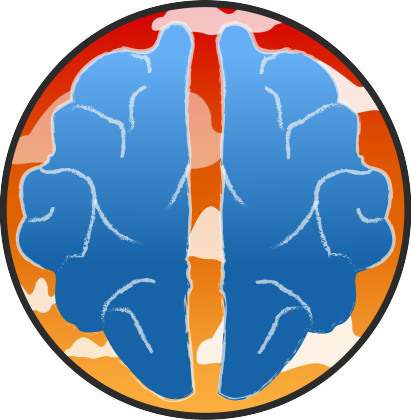
\includegraphics[width=0.2\textwidth]{pics/memoryland-logo.png}
    \end{center}
\end{wrapfigure}

Memories in the form of photos and videos are a valuable part of life, yet they are often 
lost or rarely revisited. To keep these memories alive, an appealing presentation and easy 
accessibility are essential.

The diploma project Memoryland was developed to address exactly this issue. It allows 
personal memories to be experienced in an interactive and animated form and to share them with 
others. As part of this project, a web application was created that transforms photos into 
engaging animations. Users can generate videos from these animations and share them with 
their friends.

A special focus was placed on creating an immersive experience. Memorylands enable 
users to relive their memories in virtual environments such as a forest or an island. 
Additionally, great care was taken to ensure that the functionalities are as intuitive
and comfortable as possible.

Ultimately, this project aims to make it easier for people to preserve their memories 
in a creative and entertaining way while allowing them to rediscover them effortlessly.

\newpage
\begin{spacing}{1}
    \chapter*{Zusammenfassung}
\end{spacing}
\begin{wrapfigure}{r}{0.3\textwidth}
    \begin{center}
      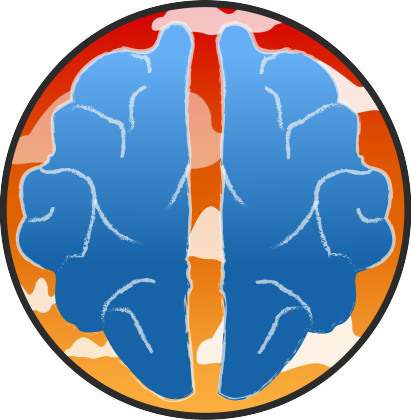
\includegraphics[width=0.2\textwidth]{pics/memoryland-logo.png}
    \end{center}
\end{wrapfigure}
Erinnerungen in Form von Fotos und Videos sind ein wertvoller Bestandteil des Lebens und doch
gehen sie oft verloren oder werden selten angesehen. Um diese Erinnerungen lebendig zu halten,
sind daher eine ansprechende Präsentation und einfache Zugänglichkeit essenziell.

Die Diplomarbeit Memoryland wurde entwickelt, um genau dieses Problem zu lösen. Sie ermöglicht es, 
persönliche Erinnerungen in einer interaktiven und animierten Form zu erleben und mit anderen zu 
teilen. Im Rahmen dieser Arbeit wurde eine Web-Anwendung erstellt, die Fotos in ansprechende 
Animationen umwandelt. Daraus können Nutzer:innen nun Videos generieren und an ihre Freunde 
weitergeben.

Besonderes wurde hierbei auf eine immersive Erfahrung geachtet. Memorylands ermöglichen es, 
Erinnerungen in einer virtuellen Umgebung, wie einem Wald oder einer Insel, zu erleben. Es
wurde auch darauf geachtet, dass die Funktionalitäten so intuitiv und gemütlich wie möglich
sind.

Schlussendlich soll unsere Arbeit es Menschen erleichtern, ihre Erinnerungen auf eine 
kreative und unterhaltsame Weise zu wahren und leicht wiederzuentdecken.



\pagestyle{plain}

\IfStrEq{\thesislang}{de}
{
	\renewcommand{\lstlistlistingname}{Quellcodeverzeichnis}
}
{
 % keep at list of listing
}

\tableofcontents
\newpage
\setcounter{RPages}{\value{page}}
\setcounter{page}{0}
\pagenumbering{arabic}
\pagestyle{scrheadings}

\begin{spacing}{1}
\chapter{Einleitung}\label{chapter:introduction}
\end{spacing}

\section{Ursprüngliche Idee}

\section{Ausgangssituation}

Herkömmliche Familien-/Fotoalben stehen normalerweise wegen ihres Gewichtes 
zuhause und falls man dann einmal einem Freund bei einer Party ein Foto schnell 
zeigen möchte, hat man eher das Handy als ein ganzes Fotoalbum dabei.
\\
Zwar gibt es schon Tools, welche die Fotos nur präsentieren, 
aber wir wollen die Fotos zeitgemäß für jeden leicht verfügbar und transportabel animieren.

\section{Untersuchungsanliegen}

Arwed Schnalzenberger:
\begin{itemize}
\item Die vorliegende Untersuchung zielt darauf ab, die effiziente Speicherung 
umfangreicher Mengen von Videos und Bildmaterial in Cloud-Umgebungen zu 
untersuchen sowie die Prozesse zur Erstellung und Bearbeitung von Videos 
auf der Backend-Ebene zu erforschen.
\end{itemize}


Isabel Schnalzenberger:
\begin{itemize}
\item Die vorliegende Untersuchung zielt darauf ab, die potenzielle Steigerung 
der Akzeptanz von Online-Darstellungen durch die Integration von 
3D-Visualisierungen einer Bildergalerie zu erforschen.
\end{itemize}

\begin{spacing}{1}
\chapter{Umfeldanalyse}
\end{spacing}
Bereits vor der Entwicklung von Memoryland, gab es bestehende Lösungen zur Verwaltung
und Präsentation von Erinnerungen. Bevor mit dem Projekt begonnen wurde, wurden
diese analysiert und die Erkenntnisse zu den Stärken und Schwächen dieser Systeme
notiert. Daraus entstanden dann die Anforderungen für das finale System.

\section{Analyse der vorhandenen Systeme}

\subsection{OneDrive}

\emph{Vorteile:}
Das System bietet eine cloudbasierte Speicherung für Bilder und andere Medien. 
So können Nutzer:innen ihre Dateien zentral ablegen und von verschiedenen Geräten aus darauf 
zugreifen.

\emph{Nachteile:}
Eine Integration von Bildern in interaktive Formate ist nicht vorhanden. 
Dadurch bleibt die Nutzung der gespeicherten Bilder auf eine einfache 
Anzeige und Verwaltung beschränkt.

\emph{Zusammenfassung:}
OneDrive bietet eine sichere und cloudbasierte Speicherung von Bildern und anderen 
Medien. Es fehlen Funktionen zur Bildbearbeitung und zur Integration von 
immersiven Formaten. \footnote{Informationen zu OneDrive stammen von \cite{MicrosoftCorporation}}

\subsection{Google Photos}

\emph{Vorteile:}
Das System stellt eine Oberfläche für eine Verwaltung und Anzeige von Bildern 
zur Verfügung. Dadurch können Nutzer:innen ihre Bilder organisieren und betrachten.

\emph{Nachteile:}
Eine Integration von Bildern in interaktive Formate ist nicht vorhanden. 
Somit ist es nicht möglich sie in erweiterte Präsentationsformen einzubinden 
und beschränkt die Nutzung der Bilder auf Verwaltungs- und Anzeigezwecke.

\emph{Zusammenfassung:}
Google Photos ermöglicht eine Verwaltung und Anzeige von Bildern, bietet jedoch 
keine Möglichkeit zur Umwandlung von Bildern in interaktive Formate. \footnote{Informationen zu Google Photos stammen von \cite{GoogleIrelandLimited}}

\subsection{Animoto}

\emph{Vorteile:}
Das System ermöglicht die Umwandlung von Bildern in animierte Diashows,
wodurch Bilder in eine dynamische Präsentationsform dargestellt werden
können.

\emph{Nachteile:}
Die erstellten Diashows enthalten jedoch keine immersiven Komponenten.

\emph{Zusammenfassung:}
Animoto bietet die Möglichkeit, Bilder in Diashows umzuwandeln. Diese Funktion gleicht 
einem animierten Fotoalbum und bietet keine immersiven Erlebnisse, wie sie in Memoryland
vorgesehen sind. \footnote{Informationen zu Animoto stammen von \cite{Animoto}}

\subsection{Zusammenfassung}

Die Marktanalyse zeigt, dass zwar verschiedene Plattformen grundlegende 
Funktionen zur Speicherung und Präsentation von Bildern bieten, jedoch 
keine immersiven Erlebnisse ermöglichen. OneDrive und Google Photos kümmern 
sich um die sichere Speicherung und Verwaltung. Animoto ermöglicht die 
Erstellung von Diashows, jedoch ohne die Möglichkeit, Bilder in virtuelle 
Umgebungen zu integrieren.

\section{Funktionale Anforderungen}

\subsection{Benutzerverwaltung}

Das System soll eine Benutzerverwaltung bereitstellen, die eine Registrierung 
und Authentifizierung ermöglicht. Für eine sichere Authentifizierung erfolgt
die Anmeldung über Azure AD B2C. Dies diemt dem Schutz der Daten der Benutzer:innen
vor Zugriff von fremden Personen.
\footnote{Mehr Informationen zu Security im Kapitel \ref{sec:security}}

\subsection{Bilder-Upload}

Nutzer:innen sollen die Möglichkeit haben, Bilder hochzuladen und in Alben zu organisieren. 
Um Erinnerungen gut organisieren zu können sollen hochgeladene Bilder und Alben 
umbenannt werden können. Darüber hinaus soll das System eine Suchfunktion bieten, 
damit Nutzer:innen ihre Bilder schnell wiederfinden können. Um den Upload-Prozess zu 
vereinfachen, soll es möglich sein, mehrere Bilder auf einmal hochzuladen. Falls 
gro\ss{}e Mengen an Bildern übertragen werden, soll eine Transaktion verwendet werden
können, sodass unterbrochene Uploads fortgesetzt werden können.

\subsection{Präsentation der Erinnerungen}

Das System soll es ermöglichen, mehrere Memorylands zu erstellen, die dem 
gleichen oder unterschiedlichen Typen angehören können. Ein Typ definiert 
dabei eine eigene Szene, zum Beispiel eine Wald- oder Inselumgebung. Nutzer:innen sollen
in einem Memoryland ihre Bilder an bestimmten Stellen platzieren können, um 
eine immersive Darstellung ihrer Erinnerungen zu ermöglichen.

\subsection{Sharing-Funktion}

Memorylands sollen mit anderen Personen geteilt werden können. Dies soll es 
Nutzern/Nutzerinnen ermöglichen, ihre Erinnerungen mit Familie und Freunden zu teilen.

\subsection{Security}

Die hochgeladenen Bilder und Alben sollen ausschlie\ss{}lich für den jeweiligen Nutzer/die
jeweilige Nutzerin verfügbar sein. Andere Nutzer sollen keinen Zugriff auf fremde Bilder 
erhalten. Wenn Memorylands mit anderen geteilt werden, soll deshalb eine deutliche Warnung 
darauf hinweisen, dass die Inhalte für andere sichtbar werden. Zudem soll es jederzeit 
möglich sein, eine Freigabe wieder zurückzuziehen, sodass geteilte Memorylands ungültig 
werden und somit nicht mehr aufrufbar sind.

\section{Nicht funktionale Anforderungen}


\subsection{Security}

Die Benutzeranmeldung erfolgt ausschlie\ss{}lich über Azure AD B2C, um eine sichere 
Authentifizierung zu gewährleisten. Hochgeladene Bilder und Memorylands dürfen nur 
für den jeweiligen Nutzer/die jeweilige Nutzerin zugänglich sein. Die Datenübertragung 
erfolgt über TLS-verschlüsselte Verbindungen (HTTPS). Zudem sollen Nutzer:innen jederzeit 
die Möglichkeit haben, ihre Daten zu löschen (``Recht auf Vergessenwerden'').

\subsection{Benutzerfreundlichkeit \& Design}

Die Webanwendung muss eine intuitive Benutzeroberfläche bieten, sodass Nutzer:innen ihre 
Erinnerungen möglichst einfach hochladen, verwalten und präsentieren können. 
Suchleisten und das Sortieren der Daten erleichtert den schnellen Zugriff auf 
unterschiedliche Inhalte.


\begin{spacing}{1}
\chapter{Architektur}\label{chapter:architecture}
\end{spacing}
\setauthor{Arwed Schnalzenberger}

\section{Architekturdiagramm}

\begin{figure} [h t]
    \centering
    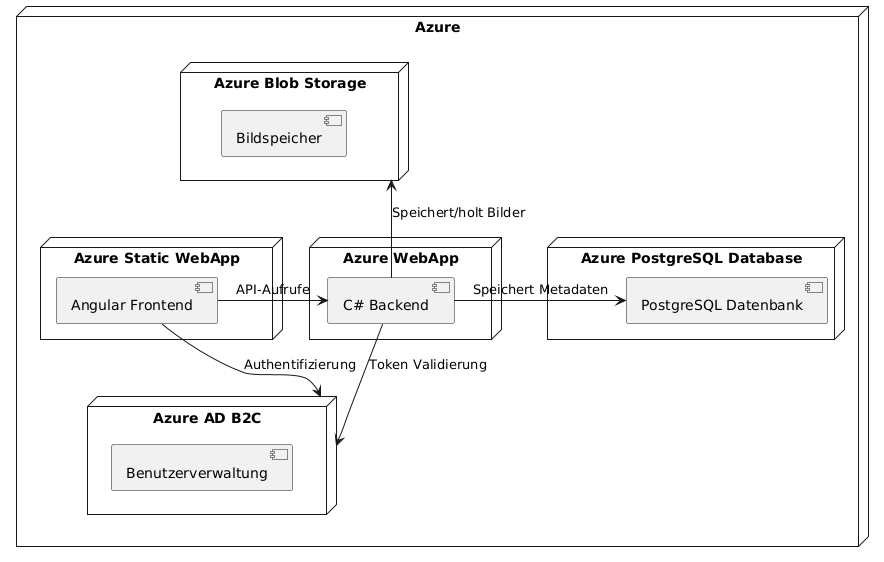
\includegraphics[scale=0.4]{puml/architecture-diagram.png}
    \caption{Architekturdiagramm}
    \label{fig:architectur-diagram}
\end{figure}

Das oben stehende Diagramm \ref{fig:architectur-diagram} zeigt die Architektur von Memoryland,
welches auf der Azure Cloud läuft. Hierbei gibt es mehrere Bestandteile, 
einschlie\ss{}lich eines Frontends, eines C\# Backends, einer Benutzerverwaltung 
über Azure AD B2C und abschlie\ss{}end einer PostgreSQL-Datenbank und einem 
Blob-Storage für die Datenhaltung.

\section{Datenhaltung}

In unserer Datenverwaltung kommen zwei Hauptkomponenten zum Einsatz, welche sich um die 
Speicherung und Verwaltung der Bilddaten kümmern. Ein Azure Blob Storage und eine Azure 
PostgreSQL Datenbank.

\subsection{Azure Blob Storage}

Hier werden die Bilder der Benutzer gespeichert. Diese werden 
ohne eine Struktur abgelegt, au\ss{}er dass für jeden Benutzer ein separater Container erstellt 
wird. Somit wird der kostenpflichtige Zugriff auf den Blob Storage minimiert und die Verwaltung
so einfach wie möglich gehalten.
\footnote{Mehr Info dazu im Kapitel: \ref{subsection:azure_blob_storage_datamodel}}
\footnote{Was ist \emph{Azure Blob Storage} und warum verwenden wir es: Kapitel \ref{subsection:azure_blob_storage}}

\subsection{Azure PostgreSQL Datenbank}

Diese Datenbank speichert die Metadaten zu den Bildern. 
Sie hält zum Beispiel Informationen darüber, in welchen Alben sich welche Erinnerungen befinden
und wem sie gehören neben anderen Details. Zusätzlich verwaltet die PostgreSQL-Datenbank die 
Struktur der Memorylands. Hier stehen unter anderem Informationen, welches Bild zu welchem 
Memoryland gehört, und wo diese im Memoryland platziert werden soll.
\footnote{Mehr Info dazu im Kapitel: \ref{chapter:datamodel}}
\footnote{Was ist \emph{Azure PostgreSQL Datenbank} und warum verwenden wir es: Kapitel \ref{subsection:postgres_db}}

\section{Benutzerverwaltung}

Die Benutzerverwaltung erfolgt über Azure AD B2C. Die Benutzer authentifizieren sich 
im Frontend mithilfe von MSAL (Microsoft Authentication Library), während das Backend 
ihre Berechtigungen gegen Azure AD B2C überprüft.
\footnote{Mehr Info zu Azure AD B2C im Kapitel: \ref{subsection:azure_ad_b2c}}
\footnote{Mehr Info zu MSAL im Kapitel: \ref{subsection:azure_ad_b2c}}

\section{Backend}

Das Backend dient dazu, die Daten von Benutzern mit den erforderlichen Berechtigungen, 
zu verwalten. Zu diesen Daten gehören unter anderem Memorylands, Alben und Bilder.
\footnote{Mehr Info dazu im Kapitel: \ref{chapter:backend-implementation}}

\section{Frontend}

Das Frontend dient als Schnittstelle zum Benutzer und bietet eine grafische 
Oberfläche zur Verwaltung ihrer Daten. Zudem ermöglicht es eine Darstellung 
der gespeicherten Bilder und Memorylands.
\footnote{Mehr Info dazu im Kapitel: \ref{chapter:frontend-implementation}}



\begin{spacing}{1}
\chapter{Datenmodell}\label{chapter:datamodel}
\end{spacing}
\setauthor{Arwed Schnalzenberger}

\begin{figure} [h t]
    \centering
    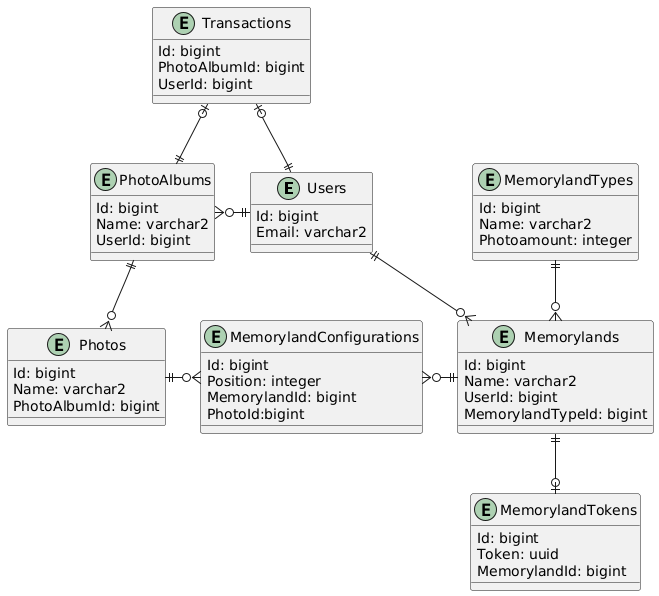
\includegraphics[scale=0.6]{puml/erd.png}
    \caption{Datenmodell}
    \label{fig:erd-diagram}
\end{figure}

Die Datenbank besteht aus insgesamt acht Tabellen, die das Backend 
für die Verwaltung von Benutzern, Fotoalben, deren Fotos und der 
Memorylands benötigt.

\section{Users}

In der Tabelle ``Users'' werden Benutzer von Memoryland gespeichert, die sich über Azure AD B2C
registriert haben. Dabei wird ein Benutzer wird mit deren Email automatisch gespeichert, sobald
er oder sie eine Aktion ausführt, die eine Speicherung im Backend erfordert. 

Der Benutzername wird nicht gespeichert, da er im Backend nicht benötigt wird und eine 
regelmäßige Aktualisierung bei Namensänderungen unnötigen Aufwand verursachen würde. Die 
E-Mail spielt in Memoryland nur als eindeutige Identifikation eines Benutzers eine Rolle.

\section{PhotoAlbums}

Diese Tabelle speichert die von Benutzern erstellten Fotoalben. Jedes Album ist eindeutig einem 
Benutzer zugeordnet, wodurch sichergestellt wird, dass ausschließlich der jeweilige Besitzer 
Zugriff darauf hat. Andere Benutzer können weder auf die Alben noch auf deren Inhalte zugreifen.

Die Alben selbst existieren als Einträge in der Datenbank, während die darin enthaltenen Fotos 
im Azure Blob Storage gespeichert werden. Das Konzept der Fotoalben wird also nur in der Datenbank 
abgebildet und hat keine direkte Entsprechung in der Speicherstruktur des Blob Storage. \footnote{\label{azure-blob-storage-note}Mehr Informationen zu ``Azure Blob Storage'' im Kapitel: \ref{subsection:azure_blob_storage_datamodel}}
Diese Struktur dient dazu, den direkten Zugriff auf den Azure Blob Storage zu minimieren und 
zu vereinfachen. Gleichzeitig ermöglicht sie dem Frontend eine sortierte und strukturierte 
Anzeige der Fotoalben.

Jeder Benutzer kann mehrere Fotoalben anlegen, wobei ein Album beliebig viele Fotos enthalten 
kann -- von keinem bis zu einer unbegrenzten Anzahl.

\section{Photos}

In dieser Tabelle werden die einzelnen Fotos mit Referenzen auf ihre jeweiligen Alben gespeichert. 
Das verwalten einzelner Fotos ist ausschließlich dem Benutzer vorbehalten, dem dieses gehört. 
Allerdings können Fotos anderen Benutzern innerhalb von Memorylands durch die Nutzung von 
SAS-Tokens angezeigt werden.

Jedes Foto gehört genau einem Album an, und innerhalb eines Albums darf kein weiteres 
Foto denselben Namen tragen. Dies gewährleistet eine eindeutige Zuordnung der Dateien für die
Benutzer.

Im Azure Blob Storage werden zur Identifikation nicht die Namen der Fotos, sondern die 
eindeutigen Identifikationsnummern verwendet. Dies ermöglicht es, dass ein Benutzer mehrere
Fotos mit identischen Namen besitzen kann, solange diese sich in unterschiedlichen Alben befinden.
\footnote{Siehe die Fußnote: \ref{azure-blob-storage-note}}

\section{Memorylands}

Ein Memoryland beinhaltet eine Sammlung von Fotos und ist immer einem bestimmten 
Memoryland-Typ zugeordnet. Der Typ eines Memorylands bestimmt unter anderem die maximale 
Anzahl an Fotos, die darin enthalten sein können.

Alle Benutzer:innen können mehrere Memorylands besitzen, die jeweils eine festgelegte Anzahl 
von Fotos an bestimmten Positionen enthalten. Die Anzahl der erlaubten Fotos pro Memoryland
hängt jeweils vom Memoryland-Typ ab.

\section{MemorylandTypes}

Diese Tabelle definiert verschiedene Typen von Memorylands. Ein Memoryland-Typ 
entspricht einer Szene in Unity und legt die maximale Anzahl an Fotos fest, die in 
einem Memoryland gespeichert werden können.

Da die Typen von den Unity-Szenen abhängen, die nur durch ein Deployment geändert werden 
können, und es keinen anderen direkten Weg gibt, festzustellen, wie viele Fotos in welcher 
Szene benötigt werden, ist es erforderlich, die Memoryland-Typen manuell in die Datenbank 
einzutragen.

\section{MemorylandConfigurations}

Diese Tabelle speichert die spezifischen Konfigurationen eines Memorylands, das heißt, 
sie definiert, welche Fotos an welchen Positionen innerhalb eines Memorylands angezeigt werden. 

Ein Memoryland kann eine beliebige Anzahl von Konfigurationen haben, wobei im Backend überprüft 
wird, ob die angegebene Position tatsächlich existiert. Zudem wird sichergestellt, dass jede 
Position innerhalb eines Memorylands nur einmal belegt wird. Es ist jedoch möglich, dass ein 
Foto in einem Memoryland mehrfach vorkommt. 

Diese Flexibilität ermöglicht es, Fotos an verschiedenen Stellen im Memoryland anzuzeigen,
ohne das die Reihenfolge der Speicherung oder anderes wichtig wäre.

\section{MemorylandTokens}

Diese Tabelle speichert die Zugriffs-Tokens eines Memorylands. Pro Memoryland kann immer nur 
ein Token gleichzeitig existieren. Benutzer:innen können mithilfe dieses Tokens auf ein 
Memoryland zugreifen und es anzeigen lassen, egal ob ihnen das Memoryland gehört oder nicht.

Die Tokens sind von der Datenbank generierte \gls{guid}s. Eine separate Tabelle für die 
Tokens wurde aus zwei wesentlichen Gründen angelegt: Zum einen ist diese Struktur eine Lösung
die eine automatische Erstellung der Tokens durch die Datenbank ermöglicht, was den 
Aufwand im Backend reduziert und eine sichere sowie eindeutige Identifikation gewährleistet. 
Zum anderen folgt die Trennung der Tokens in eine eigene Tabelle dem Prinzip der 
``Separation of Concerns''.

``\emph{Separation of Concerns}'' ist ein Prinzip der Softwareentwicklung, bei dem 
verschiedene Aspekte eines Systems oder einer Anwendung klar voneinander getrennt werden. 
In diesem Fall enthält die Tabelle der Memorylands allgemeine Informationen über die 
erstellten Memorylands, während die Tabelle der Tokens die separate Verantwortung 
für die Tokens übernimmt. Durch diese Trennung ist es einfacher neue Sicherheitsmechanismen 
oder Berechtigungsstufen oder anderes hinzuzufügen oder zu entfernen.
\footnote{Alle Informationen zu ``Separation of Concerns'' stammen von: \cite{kulkarni2003separation}}

\section{Transactions}

Diese Tabelle dient der Verwaltung von Transaktionen, die verwendet werden, um das Hochladen 
großer Fotoalben effizienter zu gestalten. Besonders bei umfangreichen Bildersammlungen, 
wie sie beispielsweise nach einer Reise oder einem Event anfallen, kann der Upload-Prozess 
durch verschiedene Faktoren unterbrochen werden -- sei es durch eine instabile 
Internetverbindung, einen Verbindungsabbruch oder anderem. Um zu verhindern, dass 
Benutzer:innen in solchen Fällen den gesamten Upload erneut starten müssen, wird ein 
Mechanismus für „Resumable Uploads“ verwendet.

In dieser Diplomarbeit werden solche Upload-Vorgänge synonym als „Transaktionen“ und 
„Resumable Uploads“ bezeichnet. Jede:r Benutzer:in kann zu einem bestimmten Zeitpunkt 
genau eine aktive Transaktion haben. In der Tabelle wird außerdem eine Referenz auf 
das jeweilige Fotoalbum gespeichert, in das die Bilder hochgeladen werden. 
Dies ermöglicht es, einen begonnenen Upload gezielt einem bestimmten Album zuzuordnen 
und den Prozess genau dort fortzusetzen, wo er unterbrochen wurde, was Benutzer:innen
dabei helfen kann, sich daran zu erinnern, wofür der Upload gedacht war.

\subsection{Probleme bei der Implementierung}
\label{subsection:implementation-problems-resumable-upload}

Ursprünglich war vorgesehen, zusätzlich den lokalen Dateipfad der hochgeladenen 
Dateien in der Datenbank zu speichern. Dieses Feature konnte jedoch aufgrund von 
Sicherheitsrichtlinien nicht umgesetzt werden, da das Speichern vollständiger 
Dateipfade potenzielle Risiken im Hinblick auf Datenschutz und Zugriffsbeschränkungen 
mit sich gebracht hätte.

Für den Upload ganzer Fotoalben wurde die HTML5-Funktion \emph{webkitdirectory} genutzt, 
die es ermöglicht, komplette Verzeichnisse auszuwählen und deren Inhalte hochzuladen. 
Allerdings erlaubt \emph{webkitdirectory} aus Sicherheitsgründen keinen Zugriff auf absolute 
Dateipfade. Stattdessen werden nur relative Pfade bereitgestellt, wodurch die 
ursprüngliche Idee, vollständige Dateipfade in der Datenbank zu speichern, technisch 
nicht umsetzbar war. \footnote{Alle Informationen zu dem ``webkitdirectory'' stammen von: \cite{MozillaFoundation}}



\begin{spacing}{1}
\chapter{Backend-Umsetzung}\label{chapter:backend-implementation}
\end{spacing}
\setauthor{Arwed Schnalzenberger}

\section{Einrichtung}

\subsection{Einrichtung des Azure Blob Storage}

Damit alles funktioniert und damit der häufige Zugriff auf die Bilder
möglichst effizient ist, wurden folgende Einstellungen im Azure Portal
konfiguriert. \footnote{Infos dazu, was Azure Blob Storage ist und anderes stammen von hier: \cite{MicrosoftCorporationd}}

\subsubsection{SAS-Tokens}

Um den Zugriff auf Bilder über Shared Access Signatures (SAS) zu ermöglichen, muss in 
die Konfiguration ``Allow storage account key access'' aktiviert werden.
\\
SAS-Tokens ermöglichen es uns, bestimmte Zugriffsrechte zu definieren, wie zum Beispiel
nur ein Lesezugriff. Das ermöglicht es unserem System, mittels Unity direkt auf die
gespeicherten Bilder zuzugreifen.
\\
Mithilfe von SAS-Tokens die im Backend generiert und an Unity übergeben werden, 
kann Unity nun auf die benötigten Bilder zugreifen, ohne vollständige Zugriffsdaten 
des Storage Accounts zu benötigen. \footnote{Alle Informationen zu SAS-Tokens stammen von: \cite{MicrosoftCorporationa}}


\subsubsection{Blob Access Tier}

Um den häufigen Zugriff auf Bilder effizienter zu gestalten, sollte in der Konfiguration 
des Blob Storage der Access Tier die Standardstufe auf ``Hot'' gesetzt werden.
\\
Ein Azure Blob Storage bietet verschiedene Speicherstufen, wie ``Hot'', ``Cool'', ``Cold'',
oder ``Archive''.Cool ist zum Beispiel Geeignet für weniger häufige Zugriffe, und hat
niedrigere Speicherkosten. 
\\
Für uns ist Hot geeignet, da mit dieser Einstellung die Bilder
für den häufigen Zugriff mit schnelleren Abrufzeiten optimiert werden. Dies führt allerdings
zu höheren Speicherkosten. \footnote{Alle Informationen zu Blob Access Tiers stammen von \cite{MicrosoftCorporationb}}


\subsubsection{CORS-Header}

CORS (Cross-Origin Resource Sharing) ist eine Sicherheitsfunktion moderner Webbrowser, 
die den Zugriff auf Ressourcen zwischen verschiedenen Ursprüngen (Domains) einschränkt.
Da Memoryland und Unity Zugriff auf Bilder aus dem Azure Blob Storage benötigen, müssen
die folgenden CORS-Einstellungen für ``Blob-Services'' benötigt.
\\
Es müssen die Spalten ``Allowed Origins'', ``Allowed Headers'' und ``Exposed Headers''
mit dem ``*'' Zeichen gefüllt werden, und Als ``Allowed Methods'', sollen ``Head'' und
``GET'' angegeben werden. Dies erlaubt den Zugriff von beliebigen Ursprüngen, mit beliebigen
Headern in der Anfrage. Weiters wird mit ``Exposed Headers'' eingestellt, dass alle 
Antwort-Header für den Client sichtbar sind und die ``Allowed Methods'' beschränkt die 
zulässigen HTTP-Methoden auf das Abrufen von Metadaten (HEAD) und das 
Laden von Bildern (GET). ``Max Age: 0'', verhindert das Caching der CORS-Vorgaben 
durch den Browser, sodass jede Anfrage die aktuellen Regeln berücksichtigt.
\\
Wenn alles eingestellt wurde, können nun Bilder aus dem Blob Storage ohne Einschränkungen 
in Memoryland angezeigt werden. \footnote{Alle Informationen zu CORS für Azure BLob Storage stammen von \cite{MicrosoftCorporationc}}


\subsection{Einrichtung von Azure PostgreSQL DB}

``Azure Database for PostgreSQL'' ist ein Datenbankdienst von Microsoft Azure, 
der auf dem Open-Source-Datenbanksystem PostgreSQL basiert \footnote{Weiter Infos zu Azure PostgreSQL: \cite{MicrosoftCorporationf}}. 
Er bietet eine Lösung für Anwendungen, die eine relationale Datenbank benötigen.
\\
Die PostgreSQL Datenbank war eine schlüssige Entscheidung aufgrund der Erfahrung der Entwickler.
\footnote{Flexible Server vs. Single Server: \cite{MicrosoftCorporatione}}

\begin{table}[h t]
    \centering
    \caption{Vergleich: Flexible Server vs. Single Server}
    \label{tab:azure-postgresql}
    \begin{tabular}{lcc}
    \hline
    \textbf{Feature}                & \textbf{Single Server} & \textbf{Flexible Server} \\ \hline
    \textbf{Betriebssystem}         & Windows                & Linux                    \\
    \textbf{Maximale Speichergrö\ss{}e} & Bis zu 16 TB           & Bis zu 64 TB             \\
    \textbf{Hochverfügbarkeit}      & Nein                   & Ja (Zonenredundant)      \\
    \textbf{Kosten}                 & 1x                     & 2x (Compute + Storage)   \\ \hline
    \end{tabular}
\end{table}

Flexible Server haben gegenüber Single Server Unterschiede. 
Der wichtigste Grund für die Entscheidung war, dass Flexible Server auf Linux basiert, 
während Single Server Windows verwendet. \footnote{Warum Linux wollten: \cite{hussain2015survey}}
\\
Au\ss{}erdem besitzen Flexible Servers eine grö\ss{}ere maximale Speichergrö\ss{}e, Zonenredundante Hochverfügbarkeit, 
wodurch Ausfälle besser abgefangen werden können. Obwohl die Kosten etwas höher sein können, 
sind Flexible Servers aufgrund dieser Punkte die bessere Wahl für unser Projekt.

\subsection{Einrichtung von Azure AD B2C}

Die Einrichtung von Azure AD B2C wurde anhand von Beispiel im folgenden MSAL-Beispiel
für Angular durchgeführt \cite{MicrosoftCorporationh}. Zusätzlich diente wurde die folgende
Website verwendet \cite{MicrosoftCorporationg}.
\\
Was ist \emph{Azure AD B2C} und warum verwenden wir es: Kapitel \ref{subsection:azure_ad_b2c}

\subsection{Einrichtung von Azure WebApp}

Die Einrichtung der Azure WebApp wurde mithilfe der folgenden Website erledigt 
\cite{MicrosoftCorporationi}.
\\
Was ist \emph{Azure WebApp} und warum verwenden wir es: Kapitel \ref{subsection:azure_web_app}


\subsection{Einrichtung von Azure Static WebApp}

Die Azure WebApp wurde nicht speziell konfiguriert, es gibt aber einige wichtige Aspekte, 
die vor dem Deployment der Angular Single Page Application beachtet werden müssen.  
\\
Damit die Static WebApp die Routen korrekt erkennt und an die Single Page Application 
weiterleitet, anstatt ``\emph{404 Not Found}''-Fehler auszugeben, muss die folgende 
Konfiguration \ref{lst:staticwebapp-config} in der Datei ``\emph{staticwebapp.config.json}'' hinterlegt werden. 
Diese Datei muss sich im Verzeichnis des Angular-Projekts befinden -- in dieser Diplomarbeit
also im Ordner ``\emph{memoryland}''. \footnote{Infos zu dem Code \ref{lst:staticwebapp-config} gibt es in diesem Video: \cite{MicrosoftCorporationj}}

\begin{lstlisting}[numbers=left,caption={staticwebapp.config.json},label={lst:staticwebapp-config}]
{
    "navigationFallback": {
        "rewrite": "/",
        "exclude": [
            "*.{png,jpg,jpeg,gif,ico,css,scss,svg,js}"
        ]
    }
}
\end{lstlisting}

Was ist \emph{Azure Static WebApp} und warum verwenden wir es: Kapitel \ref{subsection:azure_static_web_app}


\subsection{Einrichtung des Backends}

Die Einrichtung des Backends für die Diplomarbeit erfordert die Konfiguration 
der ``\emph{appsettings.json}'' Datei. In dieser Datei stehen mehrere Einstellungen,
damit Memoryland auf die Unterschiedlichen Dienste zugreifen kann. Die Konfiguration 
umfasst drei Hauptbereiche: Authentifizierung, Datenbank und den Azure Blob Storage.

\subsubsection{Authentifizierung}

Für die Authentifizierung wird Azure AD B2C genutzt, um die Benutzerverwaltung zu ermöglichen. 
In der ``\emph{appsettings.json}'' Datei sind die entsprechenden Einstellungen wie in dem folgendem
Beispiel \ref{lst:appsettings-auth-config} einzutragen. Hier werden unter anderem die Instance, ClientId und Domain des 
Azure AD B2C Verzeichnisses angegeben. Der SignedOutCallbackPath gibt den Pfad an, der nach 
der Abmeldung des Benutzers aufgerufen wird, und SignUpSignInPolicyId enthält den Namen ebenjener.
\footnote{Alle Informationen zu den Einstellungen der Authentifizierung sind hier zu finden: \cite{MicrosoftCorporationk}}

\begin{lstlisting}[numbers=left,caption={appsettings.json},label={lst:appsettings-auth-config}]
{
    "AzureAdB2C": {
        "Instance": "",
        "ClientId": "",
        "Domain": "",
        "SignedOutCallbackPath": "/signout/<SignUpSignInPolicyId>",
        "SignUpSignInPolicyId": ""
    }
}
\end{lstlisting}

\subsubsection{Datenbank}

Für die Konfiguration der Datenbank sind die entsprechenden Einstellungen wie in dem folgendem
Beispiel \ref{lst:appsettings-db-config} ebenso in der Datei ``\emph{appsettings.json}'' 
einzutragen. Es gibt sowohl eine Einstellung für den Deployment-Datenbankanschluss (Default) 
als auch eine für den lokalen Anschluss (DefaultLocal), der für Test-Zwecke verwendet wird. 
Die UseLocalDb Einstellung gibt an, ob eine lokale Datenbank verwendet werden soll, wobei
\emph{false} bedeutet, dass die Deployment Datenbank verwendet werden soll.
\footnote{Alle Informationen zu den Einstellungen der Azure Datenbank sind hier zu finden: \cite{MicrosoftCorporationl}}

\begin{lstlisting}[numbers=left,caption={appsettings.json},label={lst:appsettings-db-config}]
{
    "UseLocalDb": false,
    "ConnectionStrings": {
        "Default": "",
        "DefaultLocal": ""
    }
}
\end{lstlisting}

\subsubsection{Azure Blob Storage}

Für die Konfiguration des Azure Blob Storage sind die entsprechenden Einstellungen wie in 
dem folgendem Beispiel \ref{lst:appsettings-blob-storage-config} ebenso in der Datei 
``\emph{appsettings.json}'' einzutragen. Diese Einstellung ist notwendig, um die 
Anwendung mit dem Azure Blob Storage zu verbinden und den Zugriff auf Bilder und 
andere Dateien sicherzustellen.
\footnote{Alle Informationen zu den Einstellungen des Azure Blob Storage sind hier zu finden: \cite{MicrosoftCorporationm}}

\begin{lstlisting}[numbers=left,caption={appsettings.json},label={lst:appsettings-blob-storage-config}]
{
    "ConnectionStrings": {
        "BlobStorageDefault": "",
    }
}
\end{lstlisting}


\subsection{Einrichtung des Frontends}

% Erklärung, der ganzen environment variablen usw. + github actions


\section{Technologien}

% what is it and why do we use it

\subsection{.NET C\#}

\subsection{MSAL}

\subsection{REST}

\subsection{Postgres-DB}
\label{subsection:postgres_db}

\subsection{Azure}

\subsubsection{Blob Storage}
\label{subsection:azure_blob_storage}

\subsubsection{AD B2C}
\label{subsection:azure_ad_b2c}

https://learn.microsoft.com/en-us/azure/active-directory-b2c/overview

https://learn.microsoft.com/en-us/azure/active-directory-b2c/

\subsubsection{WebApp}
\label{subsection:azure_web_app}

\subsubsection{Static WebApp}
\label{subsection:azure_static_web_app}

\subsection{Rider}

\subsection{GitHub Actions}

\section{API-Endpoints}

\section{Integration von Azure Blob Storage}

\section{Uploads}

% Erklärung, wie genau das auch im Frontend läuft

% videos referenzieren

- 2 Teile: Postgres und BlogStorage
- BlogStorage
    - Pro User 1 Container
    - Bilder werden mit ihren Ids gespeichert + nur admin hat zugriff
    - Zugriff auf bilder erfolgt mit sas-tokens (was sind sas tokens)

\subsection{Azure Blob-Storage Datenhaltung}
\label{subsection:azure_blob_storage_datamodel}

\section{Authentifizierung}


\begin{spacing}{1}
\chapter{Frontend-Umsetzung}\label{chapter:frontend-implementation}
\end{spacing}
\setauthor{Isabel Schnalzenberger}

\section{Technologien}

\subsection{Angular}

\subsection{WebStorm}

\section{Frontend-Code Beschreibung}
\subsection{Redux-Architektur und seine drei Prinzipien}

% Links und info unter: https://2324-4bhif-wmc.github.io/2324-4bhif-wmc-lecture-notes/#_mvvm

\subsection{WebAPI Client Service}
% explain web api (explain toastservice?)

\subsection{Image Previews}
% explain image cropper --> preview image

\subsection{All Worlds Component}
% explain memoryland all worlds component
% create memoryland modal

\subsection{Edit Memoryland Config Component}
% explain edit memoryland config component

\subsection{Explore Worlds Component}
% explain memoryland explore worlds component

\subsection{Memoryland List Component}
% explain memoryland list component




\section{Benutzeroberfläche}

\subsection{Header}

\begin{figure} [h t]
    \centering
    
\includegraphics[scale=0.5]{pics/header_login.PNG}
    \caption{Header des Frontend}
    \label{fig:header-frontend}
\end{figure}

Der Header einer mit Angular entwickelten Webanwendung enthält das Logo sowie 
den Namen der Website. Durch Klicken auf das Logo oder den Namen wird der 
Benutzer zur Hauptseite der Anwendung weitergeleitet.

Zusätzlich sind Navigationslinks integriert, die den Benutzer zu verschiedenen 
Bereichen der Website führen. Die verfügbaren Links umfassen ``Home'', ``Explore 
Worlds'', ``All Worlds'', ``Memory Store'' und ``About'', diese werden später noch 
genauer erklärt. Durch das Anklicken eines dieser Links wird die entsprechende 
Seite aufgerufen. Die Seiten ``Explore Worlds'', ``All Worlds'' und ``Memory Store'' 
jedoch sind nur dann zugänglich, wenn der Benutzer sich auf der Website 
eingeloggt.


\begin{figure} [h t]
    \centering
    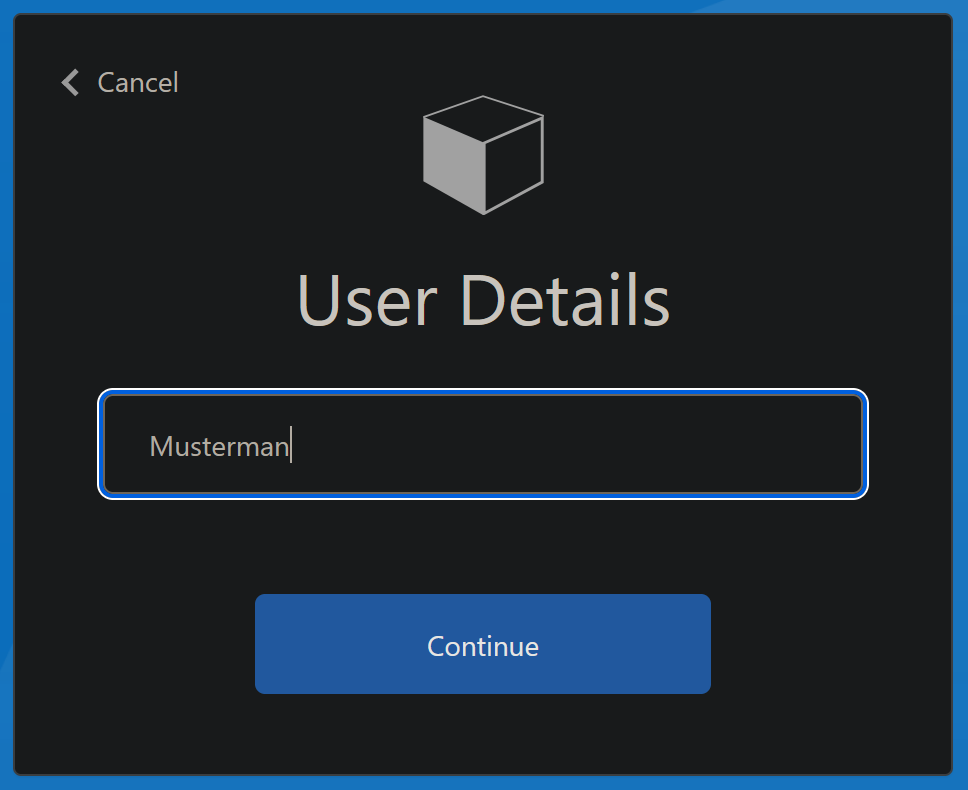
\includegraphics[scale=0.4]{pics/benutzername_aendern.PNG}
    \caption{Benutzername Ändern}
    \label{fig:benutzername-aendern}
\end{figure}

Ein Login-Button ist ebenfalls Bestandteil des Headers. Falls ein Benutzer eingeloggt 
ist, wird vor dem Login-Button ein zusätzlicher Button angezeigt, der den aktuellen 
Benutzernamen als Label enthält. Ein Klick auf diesen Button führt zu einer separaten 
Seite, auf der der Benutzername geändert werden kann.

Die Änderung des Benutzernamens erfolgt durch direktes Bearbeiten eines Textfeldes. 
Um die Änderung zu übernehmen oder zur vorherigen Seite zurückzukehren, steht ein 
``Continue''-Button zur Verfügung. Dieser speichert die Anpassung und leitet den Benutzer 
wieder auf die Website weiter. Um den vorherigen Benutzernamen jedoch beizubehalten 
oder zur vorherigen Seite zurückzukehren, steht ein Cancel-Button zur Verfügung. 

Der Header bleibt auf allen, mit Angular entwickelten, Seiten der Anwendung unverändert. 
Diese Konsistenz gewährleistet eine einheitliche Benutzerführung und erleichtert die 
Navigation innerhalb der Anwendung.


\subsection{Home}

Das Layout der Startseite ist zentriert ausgerichtet. Im oberen Bereich der Seite befindet 
sich das Logo in gro\ss{}er Darstellung, ergänzt durch den Namen der Diplomarbeit. Direkt 
darunter wird eine Willkommensnachricht angezeigt (siehe Abbildung \ref{fig:homepage}).

\begin{figure} [h t]
    \centering
    
\includegraphics[scale=0.4]{pics/home_page.PNG}
    \caption{Homepage}
    \label{fig:homepage}
\end{figure}

Am unteren Rand der Seite ist ein Link platziert, der zur Impressums- und 
Nutzungsbedingungen-Seite führt. Diese Seite ist unter der Sektion ``About'' 
näher erläutert. Alternativ kann dieselbe Seite über den About-Link im Header 
aufgerufen werden.

\subsection{About}

Die About-Seite umfasst das Impressum sowie die Nutzungsbedingungen und ist zentriert 
ausgerichtet.


Das Impressum enthält die Namen der Entwickler und deren Zuständigkeitsbereiche 
innerhalb der Website, insbesondere die Unterscheidung zwischen Frontend- und 
Backend-Entwicklung. Zusätzlich sind die vollständige Adresse der Schule mit 
Stra\ss{}enname, Hausnummer, Postleitzahl, Stadt und Land sowie die offiziellen 
Kontaktdaten der Schule, einschlie\ss{}lich Telefonnummer und E-Mail-Adresse, 
aufgeführt.

\begin{figure} [h t]
    \centering
    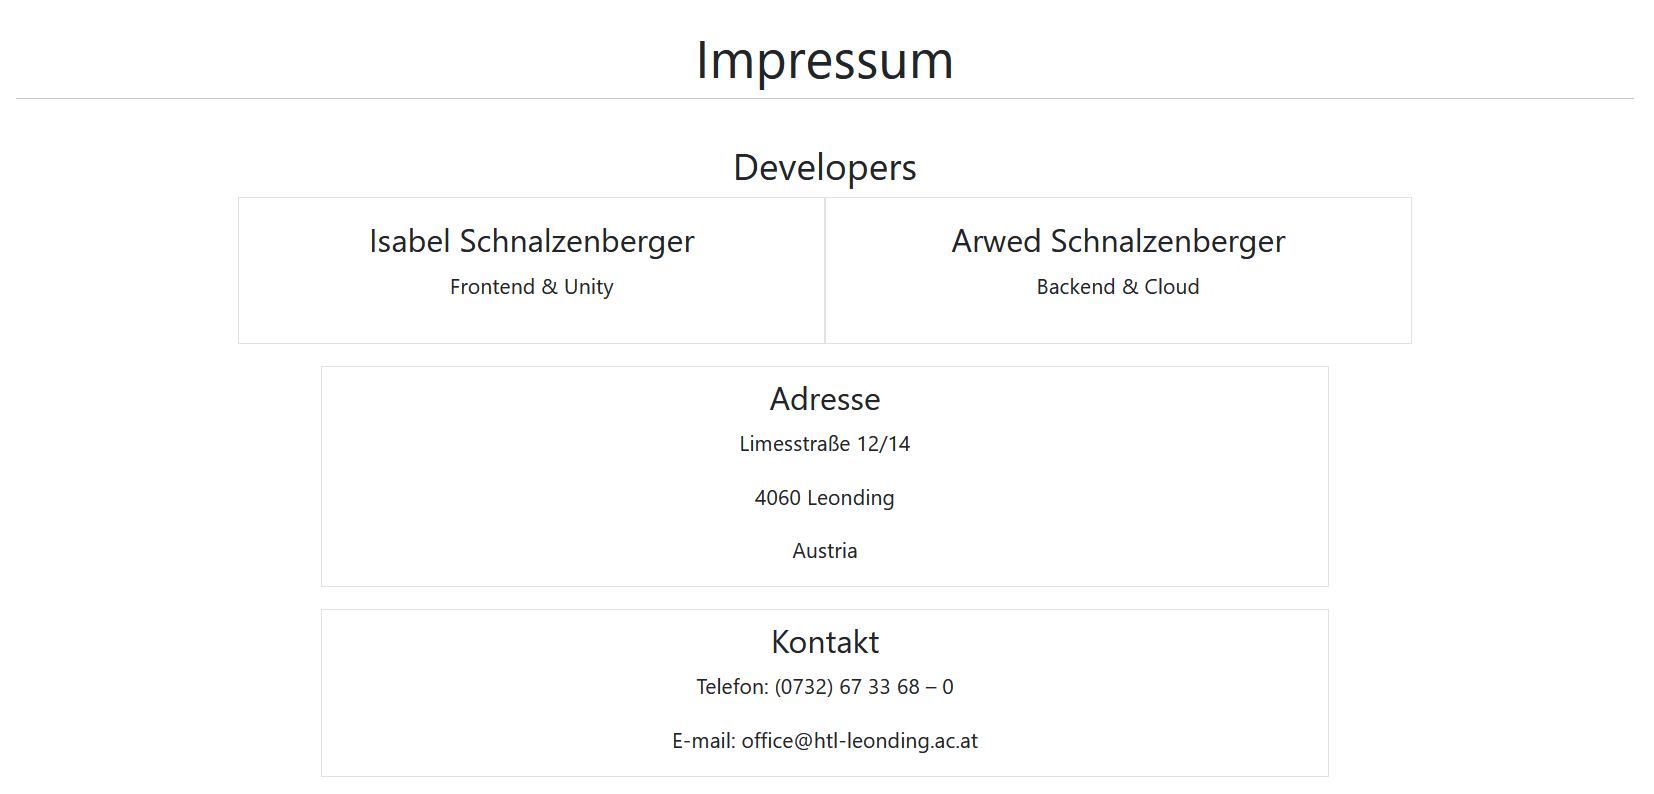
\includegraphics[scale=0.4]{pics/About_page_Impressum.PNG}
    \caption{About - Impressum}
    \label{fig:about-page-impressum}
\end{figure}



\begin{figure} [h t]
    \centering
    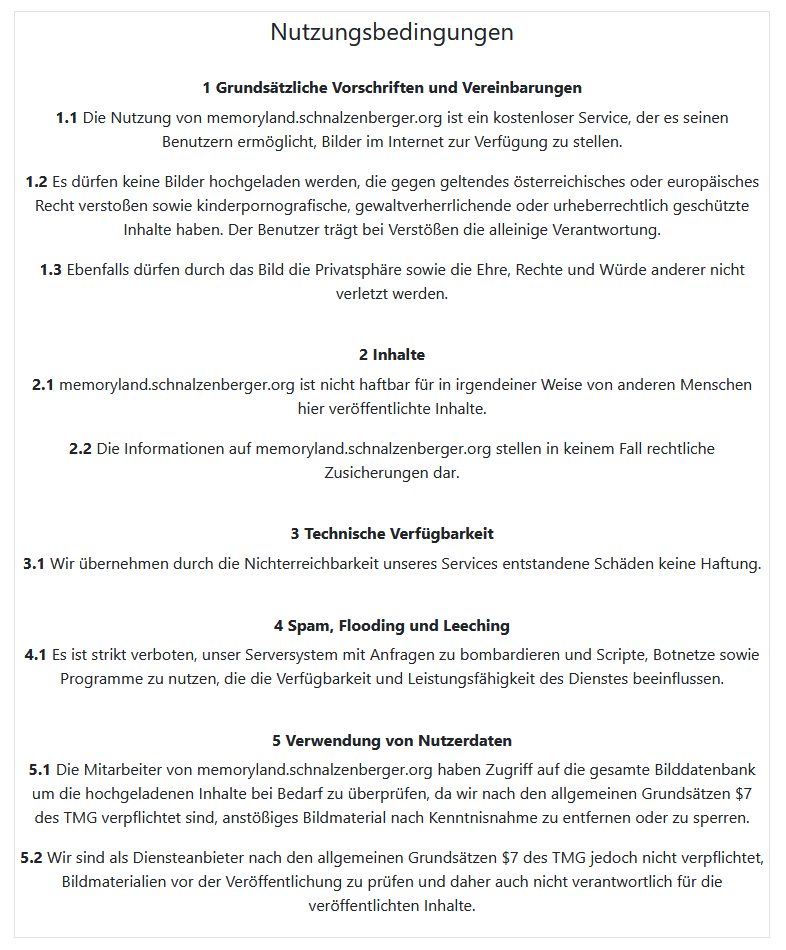
\includegraphics[scale=0.8]{pics/About_page_Nutzungsbedingungen.PNG}
    \caption{About - Nutzungsbedingungen}
    \label{fig:about-page-nutzungsbedingungen}
\end{figure}


Die Nutzungsbedingungen beinhalten allgemeine Vorschriften und Vereinbarungen zur 
Nutzung der Website. Sie umfassen spezifische Regelungen zu erlaubten und nicht 
erlaubten Inhalten, die technische Verfügbarkeit der Plattform sowie Bestimmungen 
zu unerwünschten Aktivitäten wie Spam, Flooding und Leeching. Zudem gibt es eine 
Sektion zur Verarbeitung und Nutzung von Nutzerdaten, die den Umgang mit 
personenbezogenen Informationen beschreibt.

Die Betreiber einer Website, wie der hier beschriebenen, müssen sich gegen den 
missbräuchlichen Umgang und die Verbreitung von verbotenen Materialien schützen. 
Derartige Nutzungsbedingungen gehören also genauso zum Umfang eines derartigen Projektes
wie die Implementierung selbst.






\subsection{Memory Store}

Der Memory Store ist in drei Abschnitte unterteilt und bietet verschiedene Funktionen 
zur Verwaltung von Fotoalben und Bildern. Die Benutzeroberfläche ist so gestaltet, 
dass alle wesentlichen Aktionen über interaktive Elemente, wie Buttons und 
Suchleisten, zugänglich sind.

\subsubsection{Meine Fotoalben - Das Menü}

\begin{wrapfigure}{r}{0.4\textwidth}
    \centering
    
\includegraphics[scale=0.8]{pics/memory_store_menu.PNG}
    \caption{Memory Store Menü}
    \label{fig:memory-store-menu}
\end{wrapfigure}


Dieser Abschnitt enthält mehrere Buttons zur Verwaltung und Organisation von Fotoalben 
und hochzuladenen Bildern (siehe \ref{fig:memory-store-menu}).

Der erste Button mit der Bezeichnung ``Album Erstellen'' öffnet ein Pop-up-Fenster, 
in dem der Benutzer den Namen des neuen Albums in ein Textfeld eingeben kann. 
Falls der Erstellungsprozess abgebrochen werden soll, kann entweder der 
``Cancel''-Button oder das Schlie\ss{}symbol (X) oben rechts im Pop-up-Fenster gedrückt 
werden. Nach der Eingabe des gewünschten Namens wird das Album durch Drücken 
des ``Album Erstellen''-Buttons endgültig erstellt und der Liste der vorhandenen 
Alben hinzugefügt.


\emph{Foto Hochladen}

Der zweite Button mit der Bezeichnung ``Foto Hochladen'' ermöglicht das Hochladen 
einzelner Bilder in zuvor erstellte Alben. Nach Betätigung dieses Buttons öffnet 
sich ein Pop-up-Fenster, in dem zunächst ein Album aus einer Liste bestehender Alben 
ausgewählt werden muss. Anschlie\ss{}end kann eine Datei vom eigenen Computer durch 
Drücken des ``Browse''-Buttons ausgewählt werden. Sobald eine Datei ausgewählt wurde, 
wird ihr Name in einem Textfeld angezeigt. Der Benutzer hat an dieser Stelle die 
Möglichkeit, den Namen der Datei manuell zu ändern. Das Hochladen des ausgewählten 
Bildes erfolgt schlie\ss{}lich durch Drücken des ``Foto Hochladen''-Buttons am unteren 
Rand des Pop-ups (siehe \ref{fig:memory-store-foto-hochladen}).

\begin{wrapfigure}{r}{0.4\textwidth}
    \centering
    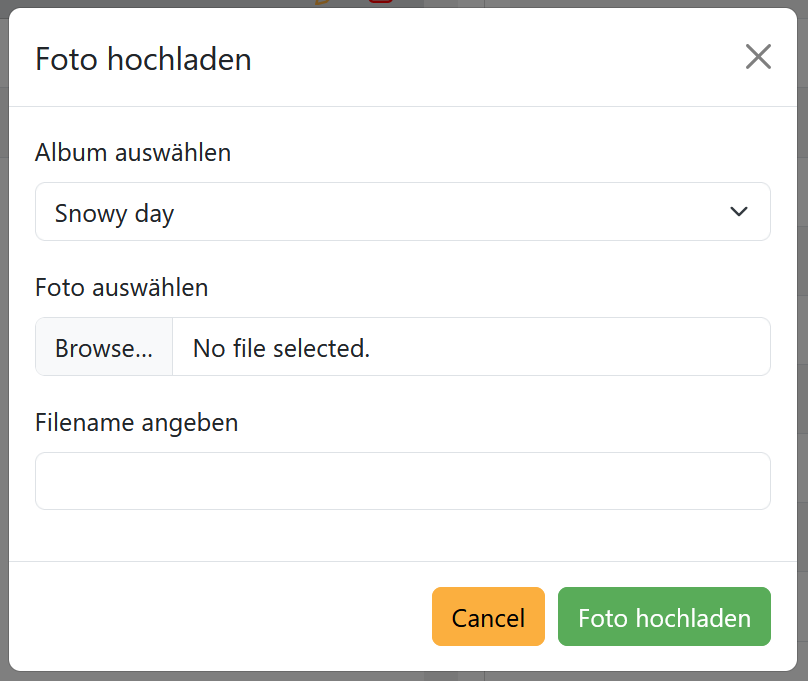
\includegraphics[scale=0.4]{pics/memory_store_teil1_button2.PNG}
    \caption{Memory Store - Foto Hochladen}
    \label{fig:memory-store-foto-hochladen}
\end{wrapfigure}


\emph{Album Hochladen}


Der dritte Menüpunkt mit der Bezeichnung ``Album Hochladen'' ermöglicht das 
Hochladen eines gesamten Albums bzw. eines lokalen Ordners mit mehreren Bildern. 
Beim Anklicken öffnet sich ein Pop-up-Fenster, in dem zunächst ein Zielalbum aus 
der Liste zuvor erstellter Alben ausgewählt werden muss. Anschlie\ss{}end kann ein 
Album vom lokalen Computer über den ``Browse''-Button ausgewählt werden. Nach der 
Auswahl wird angezeigt, wie viele Bilder sich in dem gewählten Album befinden. 
Zusätzlich gibt es eine Checkbox, die – falls aktiviert – einen resumable Upload 
ermöglicht. Diese Funktion erlaubt es, den Upload-Prozess bei einer Unterbrechung 
fortzusetzen.

\begin{wrapfigure}{r}{0.4\textwidth}
    \centering
    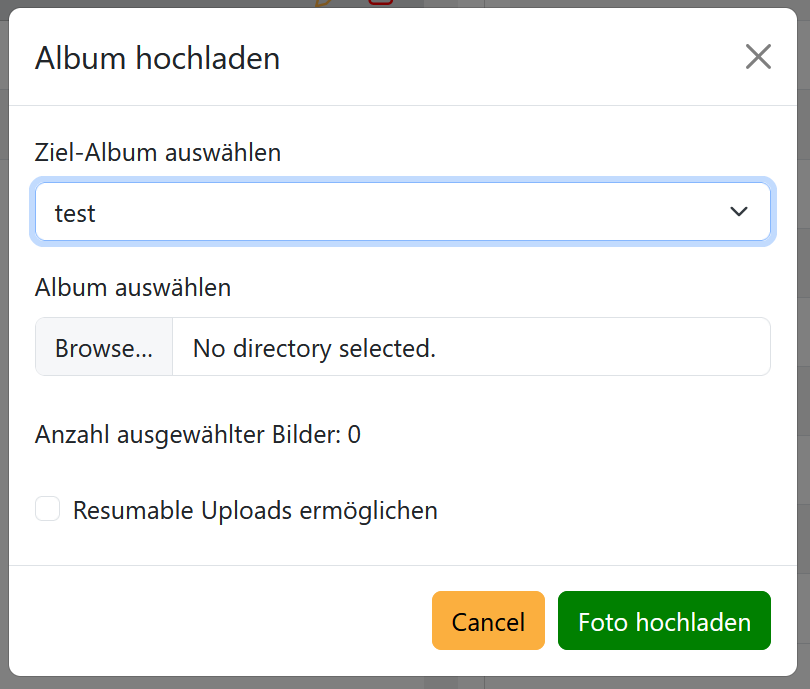
\includegraphics[scale=0.4]{pics/memory_store_teil1_button3.PNG}
    \caption{Memory Store - Album Hochladen}
    \label{fig:memory-store-album-hochladen}
\end{wrapfigure}

Nachdem der Benutzer den ``Fotos Hochladen''-Button betätigt, wird das aktuelle 
Pop-up-Fenster durch ein neues ersetzt, das eine Fortschrittsanzeige (Progress Bar) 
enthält. Diese zeigt an, wie viele der Bilder bereits hochgeladen wurden. Sobald 
der Upload abgeschlossen ist, kann der Vorgang durch Drücken des ``Exit''-Buttons 
beendet werden.

Falls der Upload während des Prozesses unterbrochen wird, kann er später fortgesetzt 
werden. Eine Unterbrechung erfolgt entweder durch das Drücken des ``Exit''-Buttons 
oder durch das Klicken au\ss{}erhalb des Pop-ups. Voraussetzung für die Fortsetzung ist, 
dass die resumable Upload-Funktion zuvor aktiviert wurde. In diesem Fall kann der 
Upload über den vierten Button ``Resume Upload'' erneut gestartet werden. Um den 
Upload fortzusetzen, muss das zuvor ausgewählte Album, von dem die Bilder stammen 
(footnote siehe discord), erneut ausgewählt werden. Nach der Auswahl kann man den 
Upload weiterführen. Während sich ein Upload im gestoppten Zustand befindet, ist das 
Hochladen weiterer Alben nicht möglich bis der laufende Upload abgeschlossen wurde.

\subsubsection{Alben}

Dieser Abschnitt enthält eine Suchleiste, mit der der Benutzer nach einem bestimmten 
Album suchen kann. Während der Eingabe von Zeichen oder Wörtern werden, automatisch 
alle Alben angezeigt, die den eingegebenen Begriff enthalten. Diese Echtzeit-Suche 
erleichtert die Navigation innerhalb der gespeicherten Alben.

\begin{wrapfigure}{r}{0.4\textwidth}
    \centering
    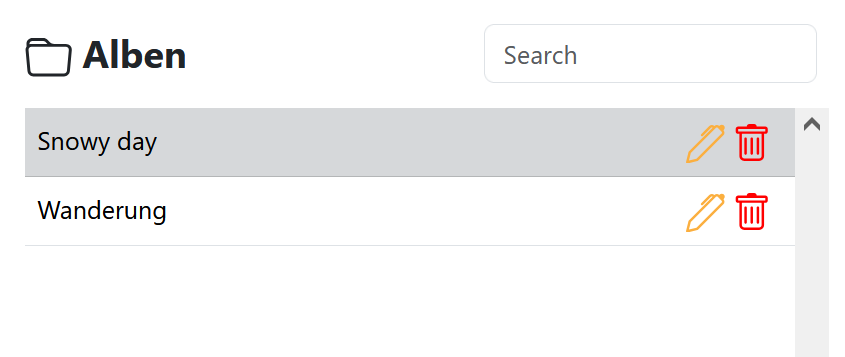
\includegraphics[scale=0.5]{pics/memory_store_teil2.PNG}
    \caption{Memory Store - Alben}
    \label{fig:memory-store-alben}
\end{wrapfigure}

Direkt unter der Suchleiste befindet sich eine Liste aller vom Benutzer erstellten 
Alben. Jedes Album wird mit seinem Namen angezeigt und hat zwei interaktive Symbole 
neben sich.

Das Stift-Symbol ermöglicht das Umbenennen des Albums. Durch Klicken auf das Symbol 
öffnet sich ein Pop-up-Fenster mit einem Textfeld, in das der neue Name eingegeben 
und bestätigt werden kann.

Das Papierkorb-Symbol ermöglicht das Löschen des Albums. Sobald der Button gedrückt 
wird, wird das Album ohne weitere Bestätigung gelöscht. Alle darin gespeicherten 
Fotos werden damit ebenfalls entfernt.

Falls ein Album durch Anklicken ausgewählt wird, erscheint sein Inhalt im dritten 
Abschnitt, der die enthaltenen Fotos anzeigt.

\subsubsection{Fotos}

\begin{figure} [h t]
    \centering
    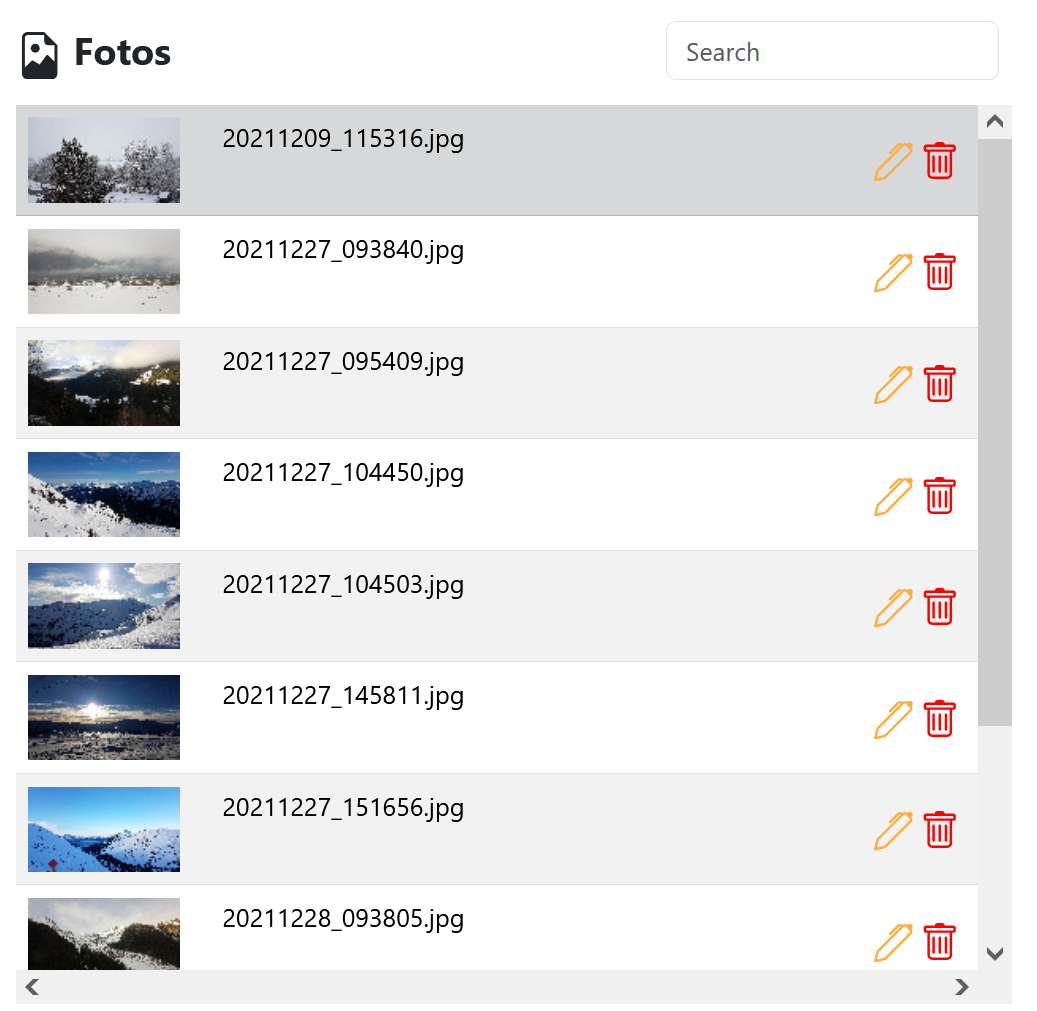
\includegraphics[scale=0.7]{pics/memory_store_teil3.PNG}
    \caption{Memory Store - Fotos}
    \label{fig:memory-store-fotos}
\end{figure}

Im oberen Bereich befindet sich eine Suchleiste, die identisch zur Suchfunktion in 
Abschnitt 2 arbeitet. Hier kann der Benutzer gezielt nach bestimmten Fotos innerhalb 
des gewählten Albums suchen.

Wenn kein Album in Abschnitt ``Alben'' ausgewählt wurde, bleibt dieser Bereich leer. 
Sobald jedoch ein Album ausgewählt wurde, werden die darin enthaltenen Fotos im 
unteren Bereich inklusive kleiner Vorschaubilder aufgelistet.

Jedes Foto wird mit seinem Namen angezeigt und besitzt zwei interaktive Symbole direkt 
daneben.

Das Stift-Symbol ermöglicht das Umbenennen des Bildes. Durch Anklicken wird ein Textfeld 
geöffnet, in das der neue Name eingetragen werden kann.

Das Papierkorb-Symbol löscht das Foto dauerhaft. Das Bild wird nach Betätigung des Symbols 
ohne weitere Bestätigung aus dem Album entfernt.

Falls ein Foto durch Anklicken ausgewählt wird, öffnet sich eine Ansicht mit dem Bilde, 
in der der Dateiname zusätzlich angezeigt wird. 

\subsection{All Worlds}

\begin{wrapfigure}{r}{0.4\textwidth}
    \centering
    
\includegraphics[scale=0.7]{pics/all_worlds_teil1.PNG}
    \caption{All Worlds - Menü}
    \label{fig:all-worlds-menu}

    \vspace{1cm}

    \centering
    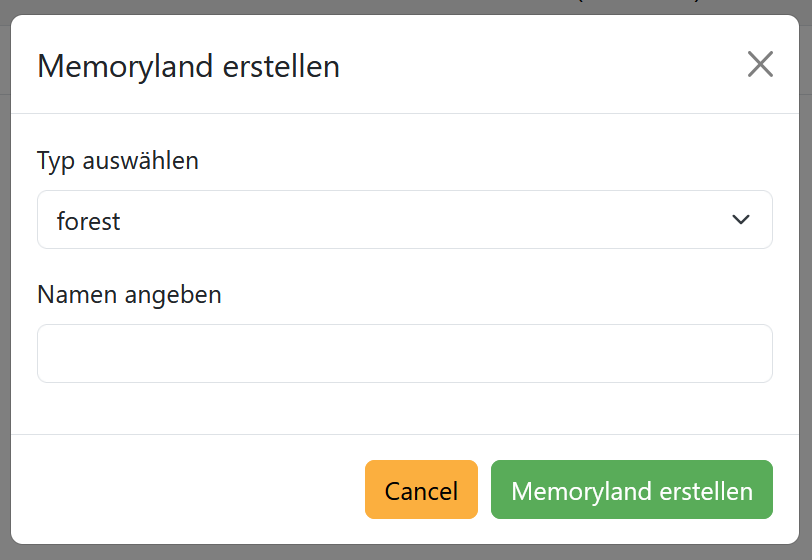
\includegraphics[scale=0.5]{pics/all_worlds_teil1_button.PNG}
    \caption{Memoryland erstellen}
    \label{fig:all-worlds-memoryland-erstellen}

\end{wrapfigure}

Die Erstellung und Verwaltung von Memorylands erfolgt ausschlie\ss{}lich auf der Seite 
``All Worlds''. Diese Seite ist in zwei Hauptabschnitte unterteilt, die 
unterschiedliche Funktionen bieten.

\subsubsection{Meine Erinnerungen}

% figure ist oben dabei
%\begin{wrapfigure}{r}{0.4\textwidth}
%\end{wrapfigure}

Der erste Abschnitt trägt die Bezeichnung ``Meine Erinnerungen''. Hier befindet 
sich ein Button mit der Aufschrift ``Memoryland Erstellen''. Durch das Anklicken 
dieses Buttons wird ein Pop-up-Fenster geöffnet, in dem verschiedene Einstellungen 
für das neue Memoryland vorgenommen werden können. Es enthält eine Auswahlmöglichkeit, 
in der der gewünschte Typ des Memorylands bestimmt werden kann. Zur Verfügung stehen 
zwei verschiedene Typen: ``Forest'' und ``Island''. Diese Typen definieren die 
visuelle Darstellung der Bilder innerhalb des Memorylands. Zusätzlich ist ein 
Textfeld vorhanden, in das der gewünschte Name des Memorylands eingetragen werden 
kann.



\subsubsection{Memorylands}

Der zweite Abschnitt der Seite trägt den Namen ``Memorylands'' und dient der 
Verwaltung bereits erstellter Memorylands. Um ein bestimmtes Memoryland schnell 
zu finden, steht eine Suchleiste zur Verfügung. Durch das Eintippen eines Namens 
oder einzelner Zeichen werden bereits während der Eingabe passende Ergebnisse 
gefiltert und angezeigt. Direkt unterhalb dieser Suchleiste werden alle zuvor 
erstellten Memorylands in einer strukturierten Übersicht dargestellt. Jedes 
Memoryland wird dabei mit mehreren Informationen versehen. Dazu gehören der 
Name des Memorylands, der gewählte Typ sowie die maximale Anzahl an Fotos, die 
innerhalb dieses Memorylands gespeichert werden können. Zusätzlich befinden sich 
neben diesen Informationen drei verschiedene Symbole, die für die Bearbeitung und 
Verwaltung der Memorylands vorgesehen sind.

\begin{figure} [h t]
    \centering
    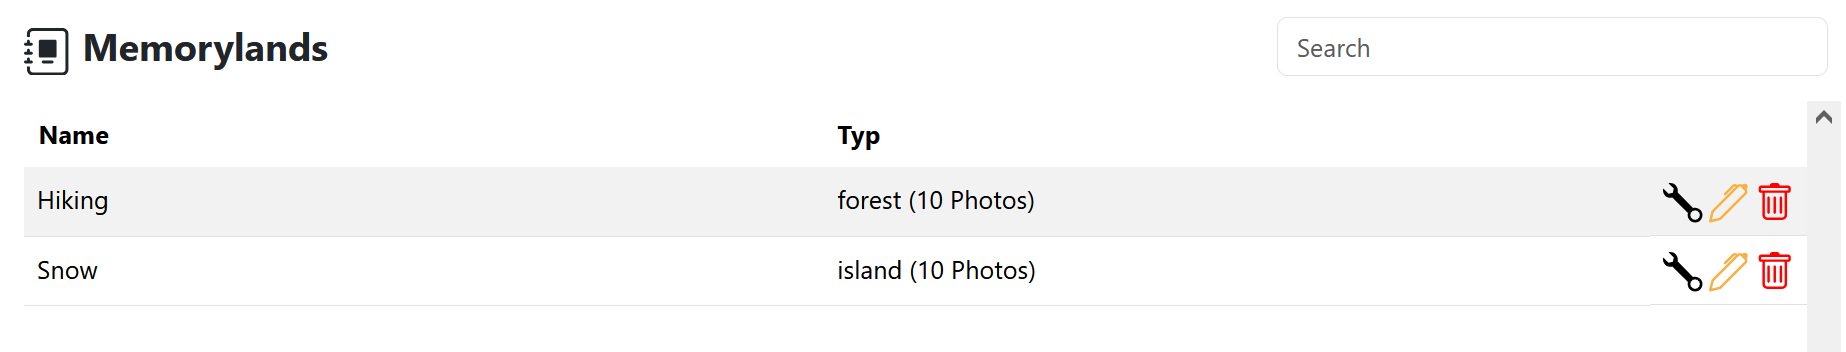
\includegraphics[scale=0.6]{pics/all_worlds_teil2.PNG}
    \caption{Memorylands Übersicht}
    \label{fig:all-worlds-memorylands}
\end{figure}

Das mittlere Symbol ist ein Stift-Icon. Durch das Anklicken dieses Symbols wird 
die Möglichkeit geboten, den Namen des Memorylands zu ändern. Ein Eingabefeld 
erscheint, in das ein neuer Name eingetragen werden kann. Das nächste Symbol ist 
ein Papierkorb-Icon. Wenn dieses Symbol betätigt wird, wird das Memoryland 
unwiderruflich gelöscht. Eine zusätzliche Sicherheitsabfrage erfolgt dabei 
nicht, sodass das Memoryland sofort aus der Liste entfernt wird. 

Das forderste Symbol ist ein Schraubenschlüssel-Icon. Durch das Anklicken dieses 
Symbols öffnet sich ein weiteres Pop-up-Fenster, das zusätzliche Bearbeitungsoptionen 
bereitstellt. 

\subsubsection{Memorylands editieren}

In diesem Pop-up-Fenster kann ein bestehendes Fotoalbum aus der eigenen Sammlung 
ausgewählt werden, aus dem Bilder in das Memoryland eingefügt werden sollen. Um 
Bilder in das Memoryland zu integrieren, steht eine Drag-and-Drop-Funktion zur 
Verfügung. 

Bilder können aus einem oberen Bereich des Fensters in einen unteren 
Bereich verschoben werden. Falls sich eine gro\ss{}e Anzahl an Bildern in dem 
ausgewählten Album befindet, kann eine zusätzliche Suchleiste genutzt werden, 
um gezielt nach bestimmten Bildern zu suchen.

\begin{figure} [h t]
    \centering
    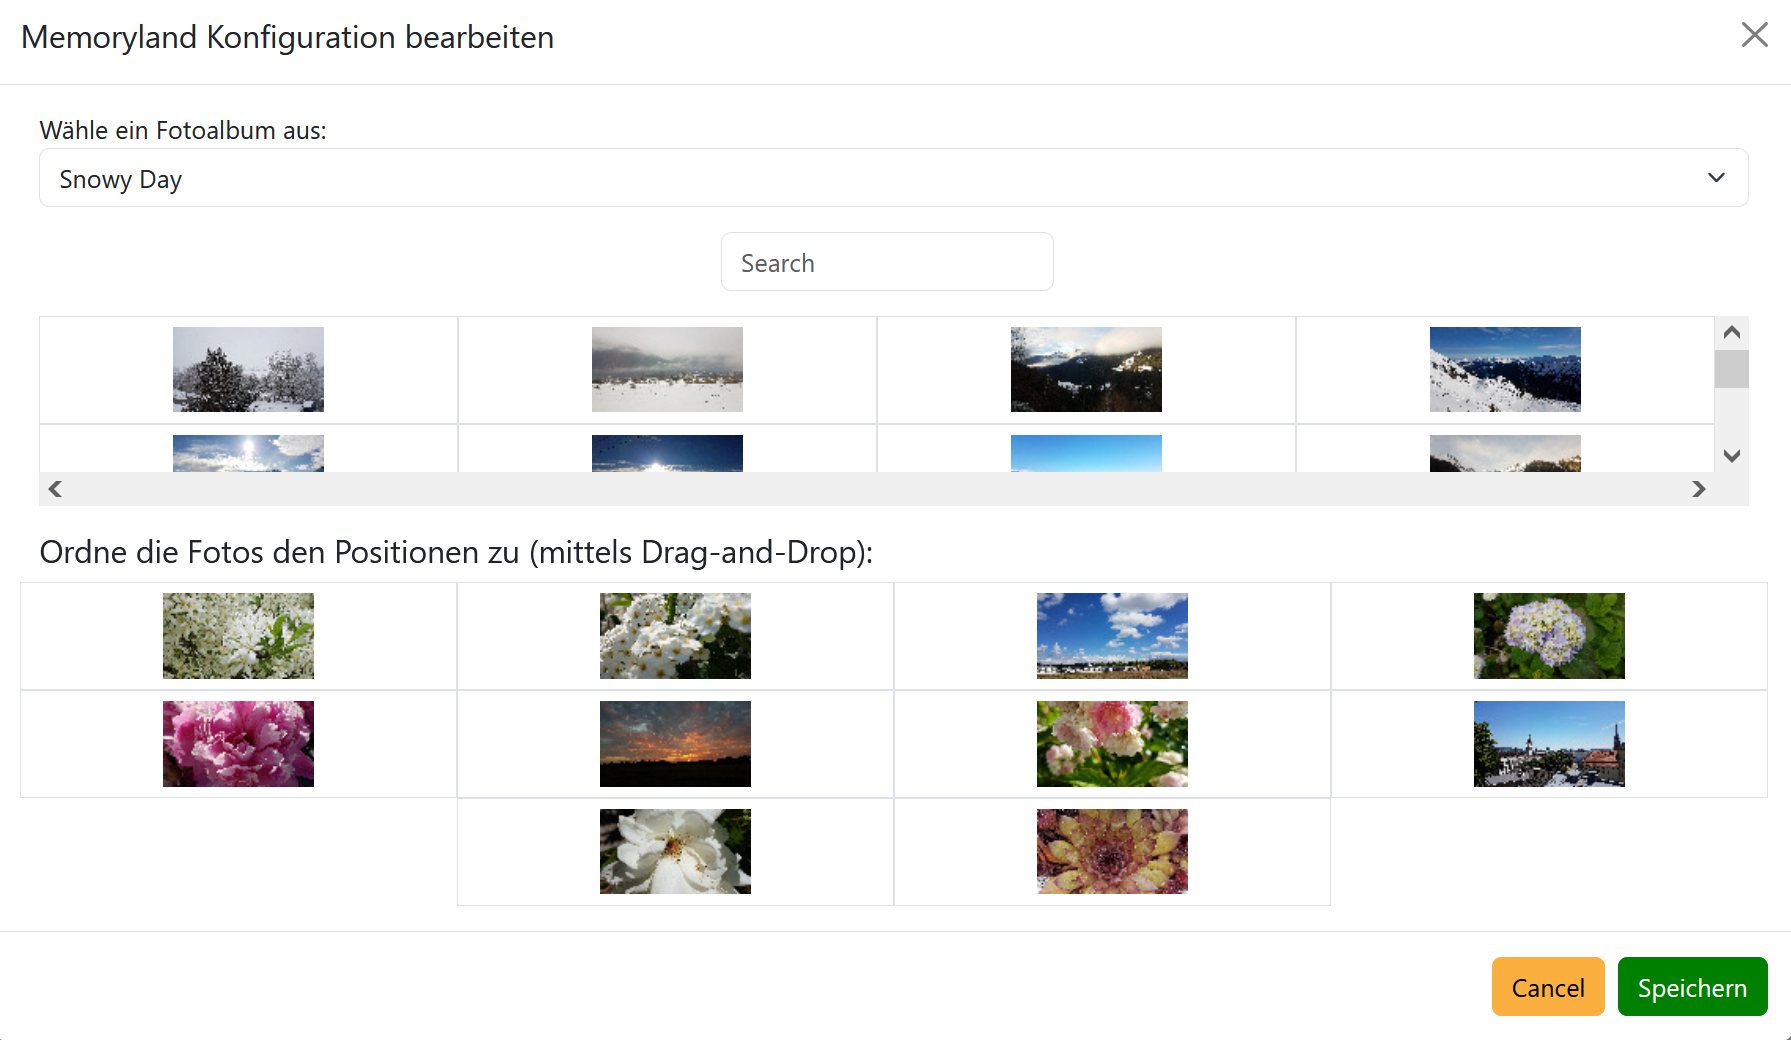
\includegraphics[scale=0.6]{pics/all_worlds_teil2_button.PNG}
    \caption{Memorylands editieren}
    \label{fig:all-worlds-memorylands-editieren}
\end{figure}


\subsection{Explore Worlds}


\begin{figure} [h t]
    \centering
    
\includegraphics[scale=0.45]{pics/explore_worlds_header.PNG}
    \caption{Explore Worlds - Zugang}
    \label{fig:explore-worlds-overview}
\end{figure}

Nachdem ein Memoryland erfolgreich erstellt wurde, kann es über die Übersicht in ``All Worlds'' aufgerufen werden. 
Sobald der Nutzer auf den Namen eines Memoryland klickt, erfolgt eine automatische Weiterleitung 
zur Seite ``Explore Worlds''. Dort wird das ausgewählte Memoryland sofort geladen 
und visuell dargestellt. Dies ermöglicht eine interaktive Betrachtung der gespeicherten 
Erinnerungen innerhalb der gewählten Umgebung.

\ref{fig:explore-worlds-loading-unity} zeigt das Unity WebGL geladen wird ....


\ref{fig:explore-worlds-loading} zeigt die beladung der szene und der daten aus dem Backend und der fotos..... siehe \ref{subsec:unity-startup-scene}


\begin{figure} [h t]
    \centering
    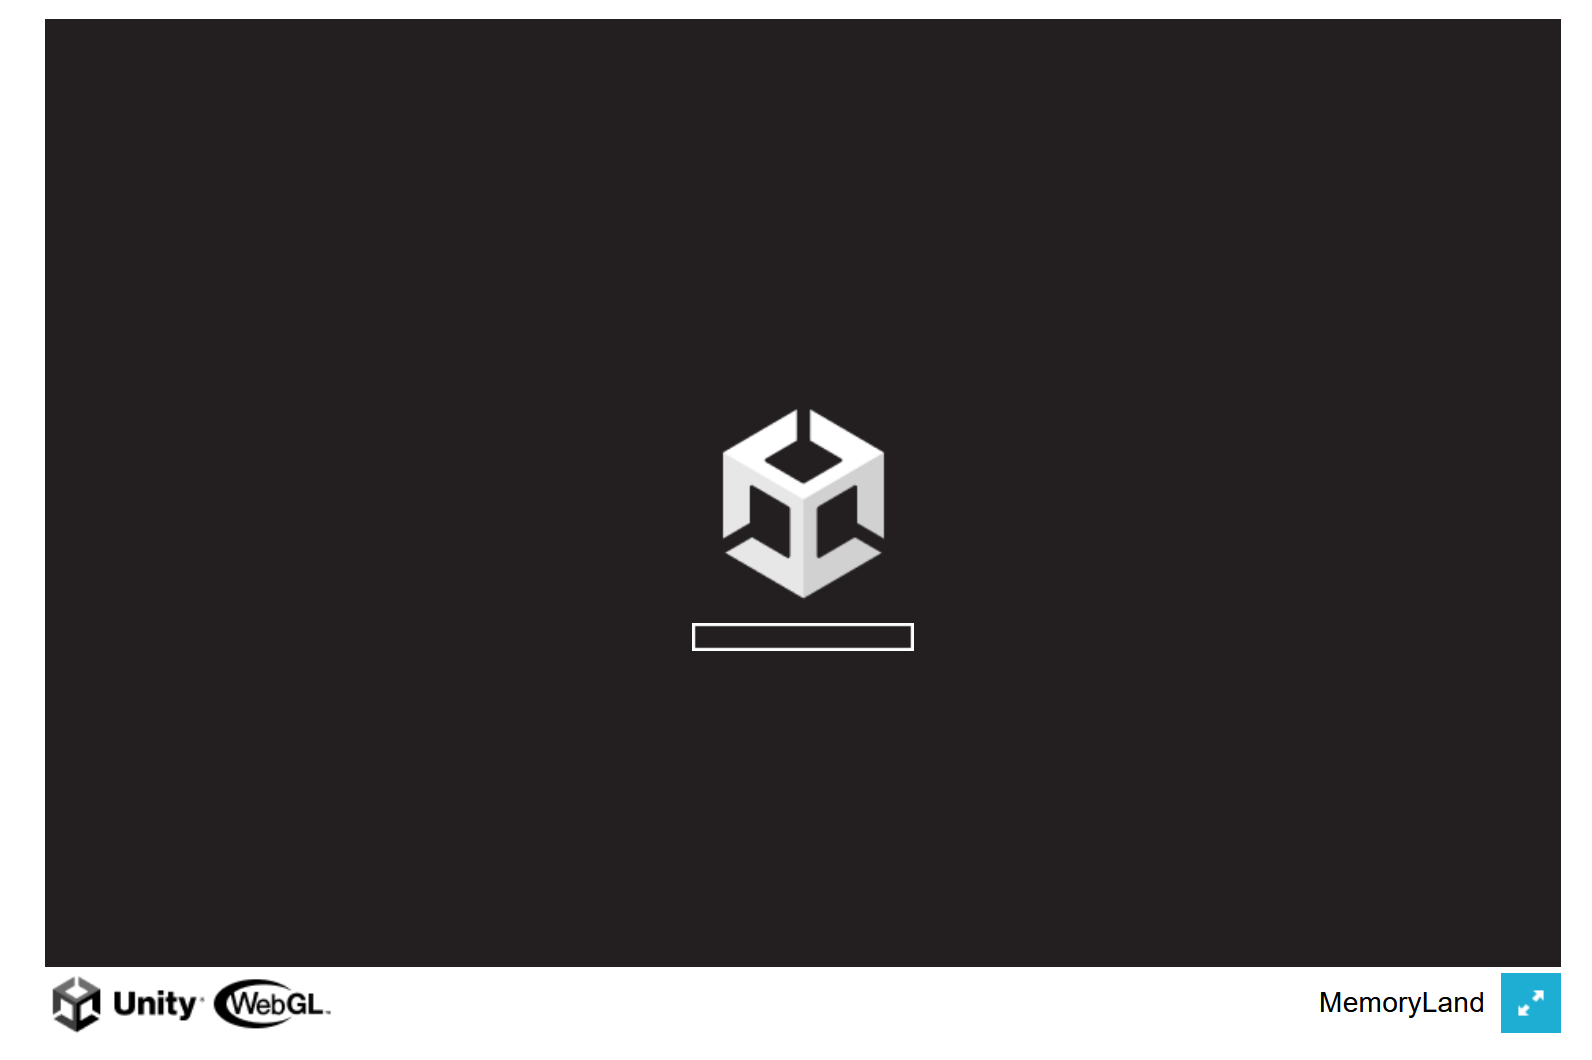
\includegraphics[scale=0.5]{pics/explore_worlds_loading_unity.PNG}
    \caption{Explore Worlds Loading Unity}
    \label{fig:explore-worlds-loading-unity}

    \vspace{1cm}

    \centering
    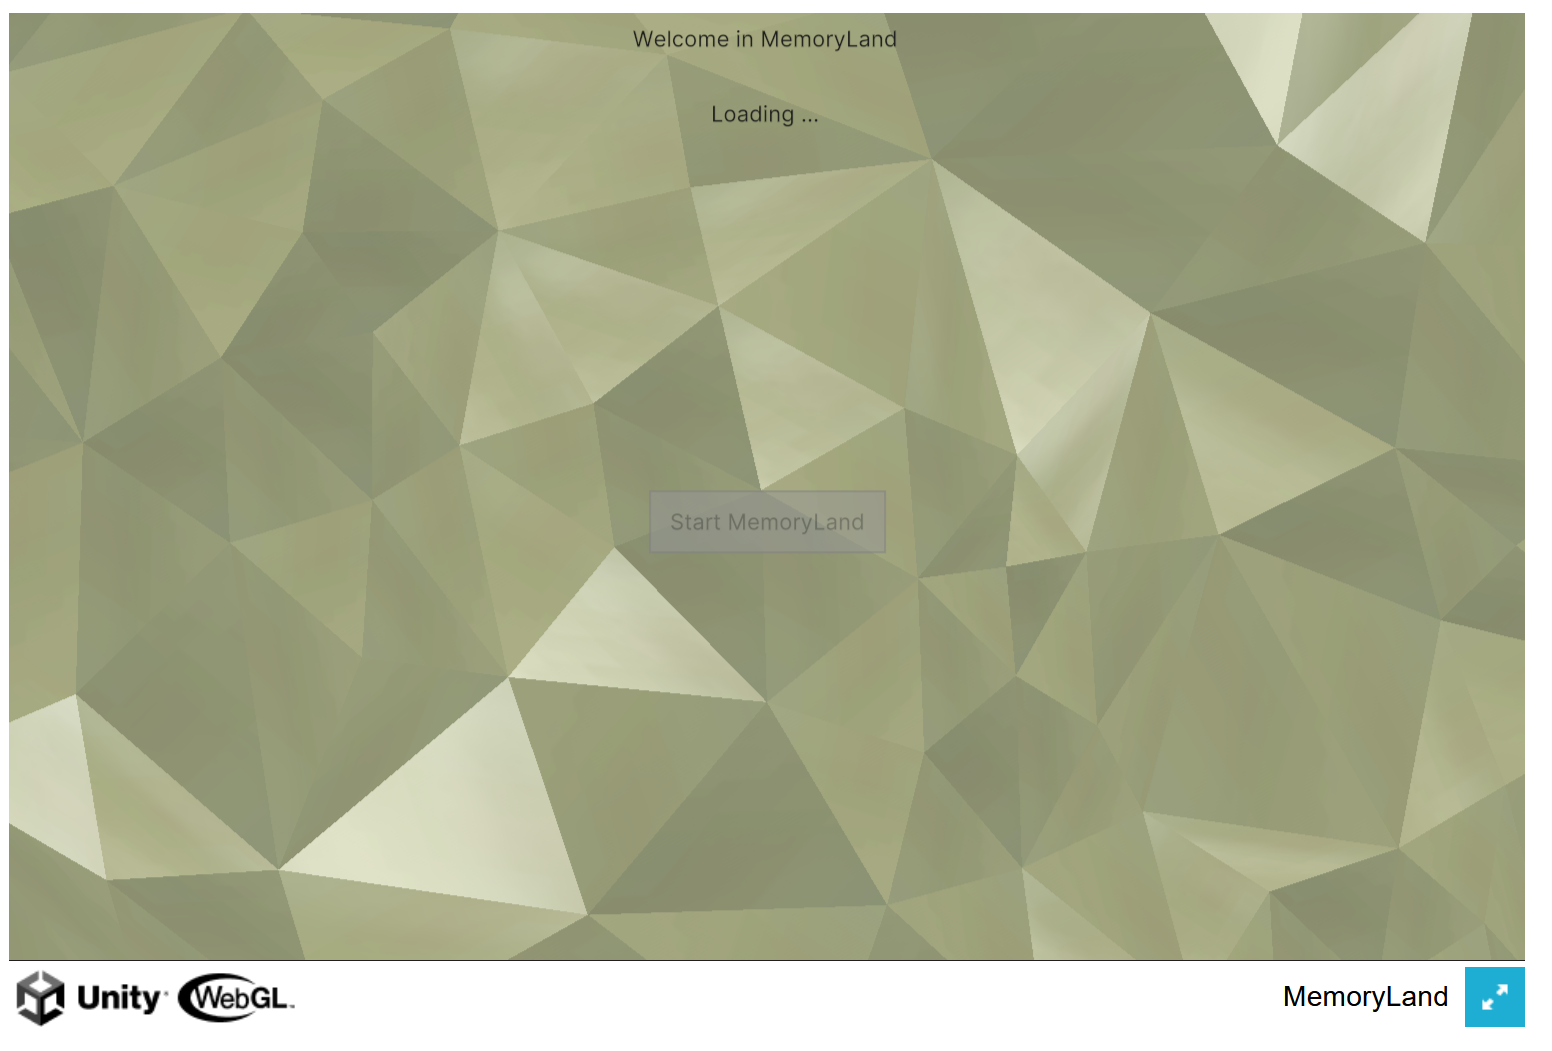
\includegraphics[scale=0.5]{pics/explore_worlds_loading.PNG}
    \caption{Explore Worlds Loading}
    \label{fig:explore-worlds-loading}
\end{figure}


\ref{fig:explore-worlds-forest} zeigt den durchlauf einer wald szene ... blabla


\ref{fig:explore-worlds-island} zeigt den durchlauf einer insel szene ....


\begin{figure} [h t]
    \centering
    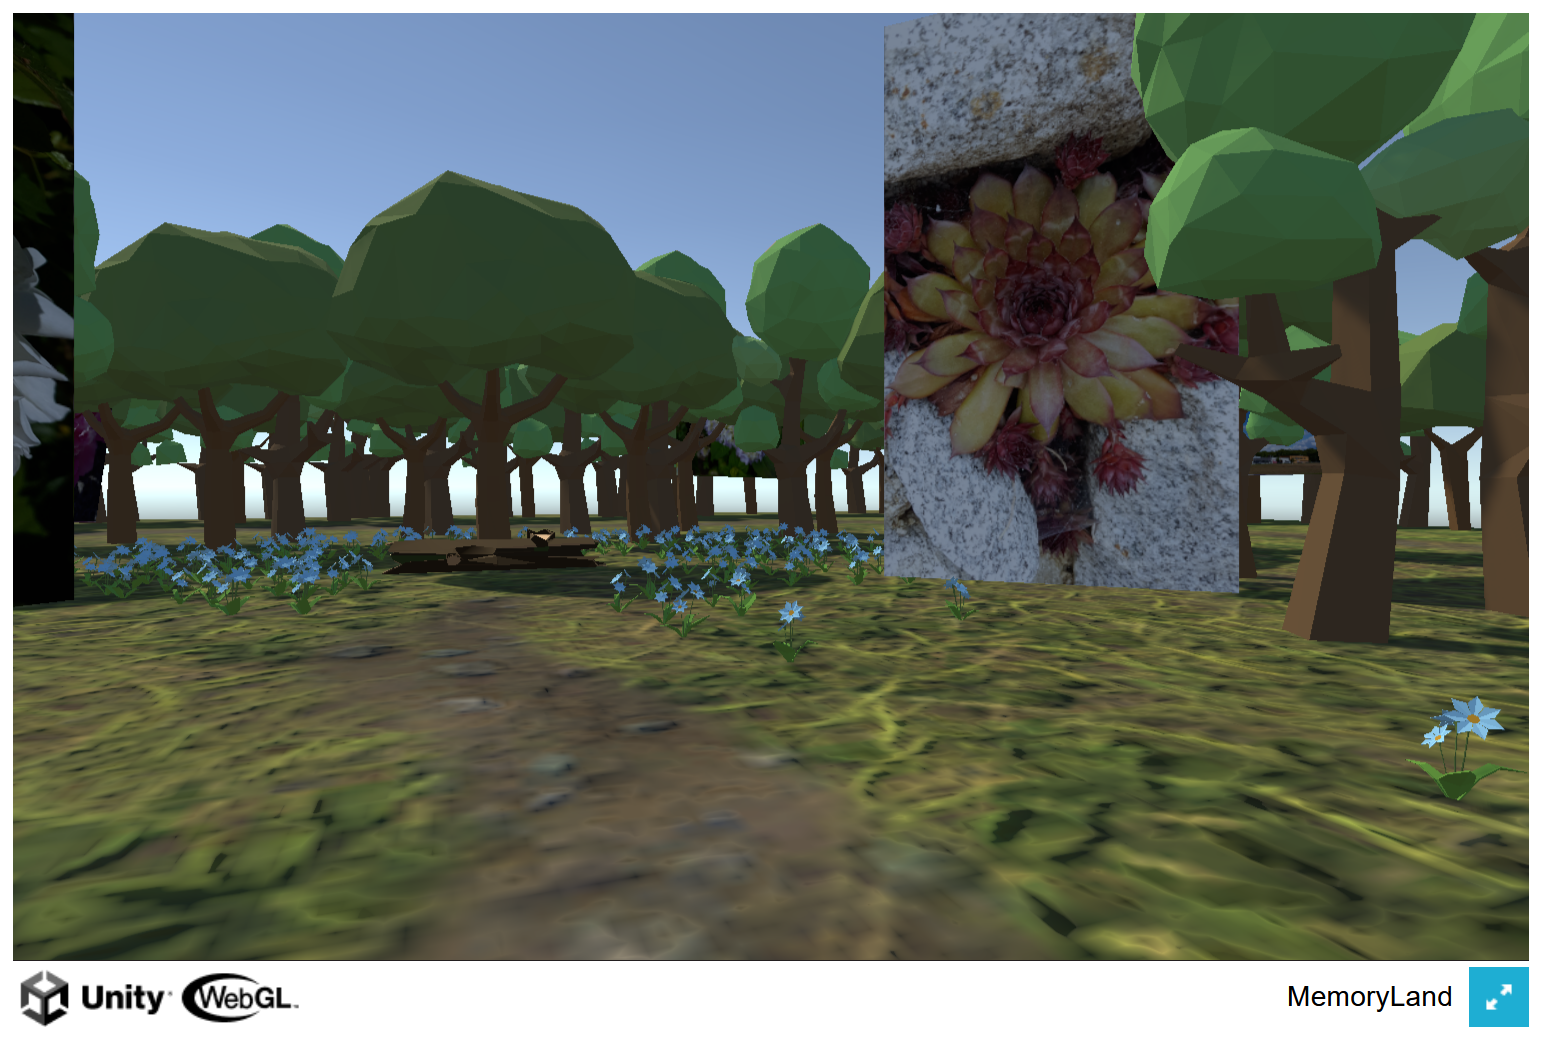
\includegraphics[scale=0.5]{pics/explore_worlds_forest.PNG}
    \caption{Explore Worlds Forest}
    \label{fig:explore-worlds-forest}

    \vspace{1cm}
    
    \centering
    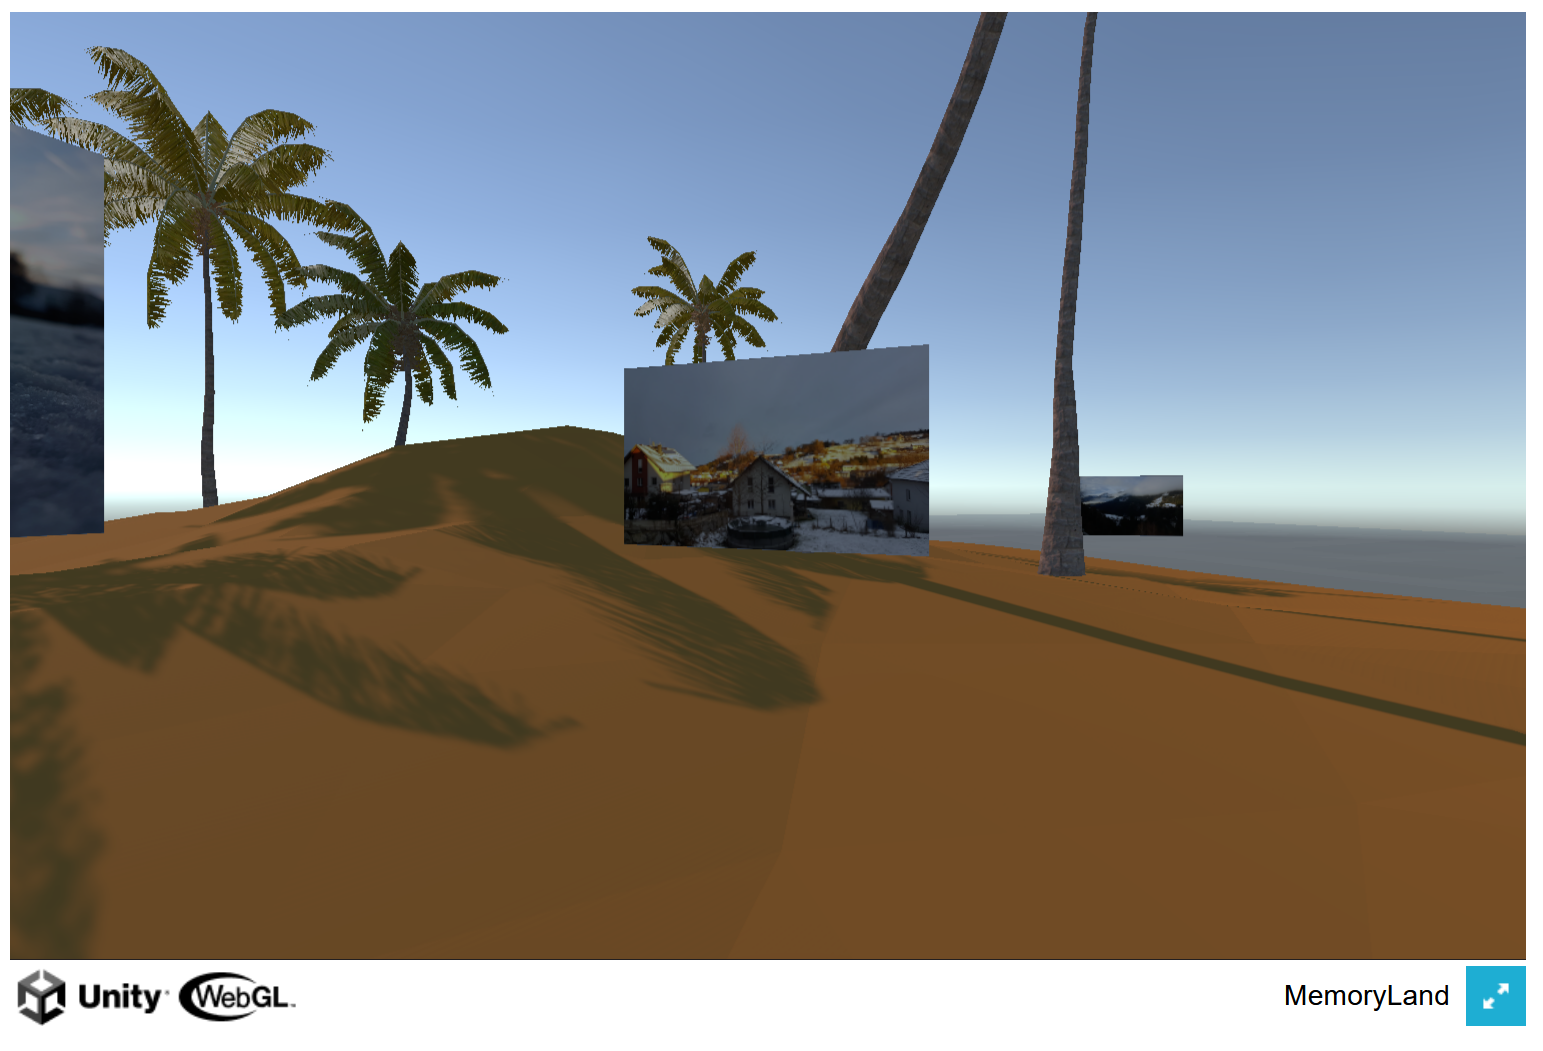
\includegraphics[scale=0.5]{pics/explore_worlds_island.PNG}
    \caption{Explore Worlds Island}
    \label{fig:explore-worlds-island}
\end{figure}





\clearpage










\subsection{Toasts}

Toasts sind eine \emph{visuelle Rückmeldung} für Benutzer und zeigen an, ob eine Aktion 
erfolgreich war, fehlgeschlagen ist oder allgemeine Informationen enthält.  

Die Toast-Nachrichten erscheinen im oberen rechten Bereich der Website, jedoch 
unterhalb des Headers. Sie bleiben für eine bestimmte Zeit sichtbar und verschwinden 
automatisch. Alternativ können sie durch das Klicken auf ein ``X''-Symbol manuell 
geschlossen werden.  

Es gibt drei verschiedene Farbvarianten, die jeweils eine spezifische Bedeutung 
haben. Ein grüner Toast signalisiert ``Success'' und zeigt an, dass eine Aktion 
erfolgreich abgeschlossen wurde, beispielsweise die Erstellung eines Albums oder 
eines Memorylands. Ein roter Toast steht für ``Error'' und bedeutet, dass während 
eines Prozesses ein Fehler aufgetreten ist, wodurch der Vorgang unterbrochen oder 
gestoppt wurde. Ein blauer Toast steht für ``Information'' und enthält eine neutrale 
Nachricht, die lediglich eine Mitteilung darstellt, ohne dass es sich um eine 
Erfolgsmeldung oder eine Fehlermeldung handelt.

Durch die Farbkennzeichnung wird die Bedeutung der Toast-Nachricht sofort erkennbar. 
Dies verbessert die Benutzerfreundlichkeit, da Informationen schnell erfasst werden 
können, ohne dass zusätzliche Interaktionen erforderlich sind.









\begin{spacing}{1}
\chapter{Unity-Umsetzung}\label{chapter:unity-implementation}
\end{spacing}
\setauthor{Isabel Schnalzenberger}

\section{Technologien}

\subsection{Unity}

\textbf{Unity} ist eine Entwicklungsumgebung (\Gls{ide}) für Spiele, auch als \textbf{Spiel-Engine (bzw. Gameengine)} bekannt, die von Unity Technologies mit Hauptsitz in San Francisco entwickelt wurde. Diese vielseitige Plattform ermöglicht die Erstellung von Spielen und interaktiven 3D-Grafik-Anwendungen für verschiedene Zielplattformen, darunter PCs (Windows und Mac), Spielkonsolen, mobile Geräte und Webbrowser.\footnote{Alle Infos zu Unity stammen von: \cite{UnityDocs}}

\begin{figure} [h t]
    \centering
    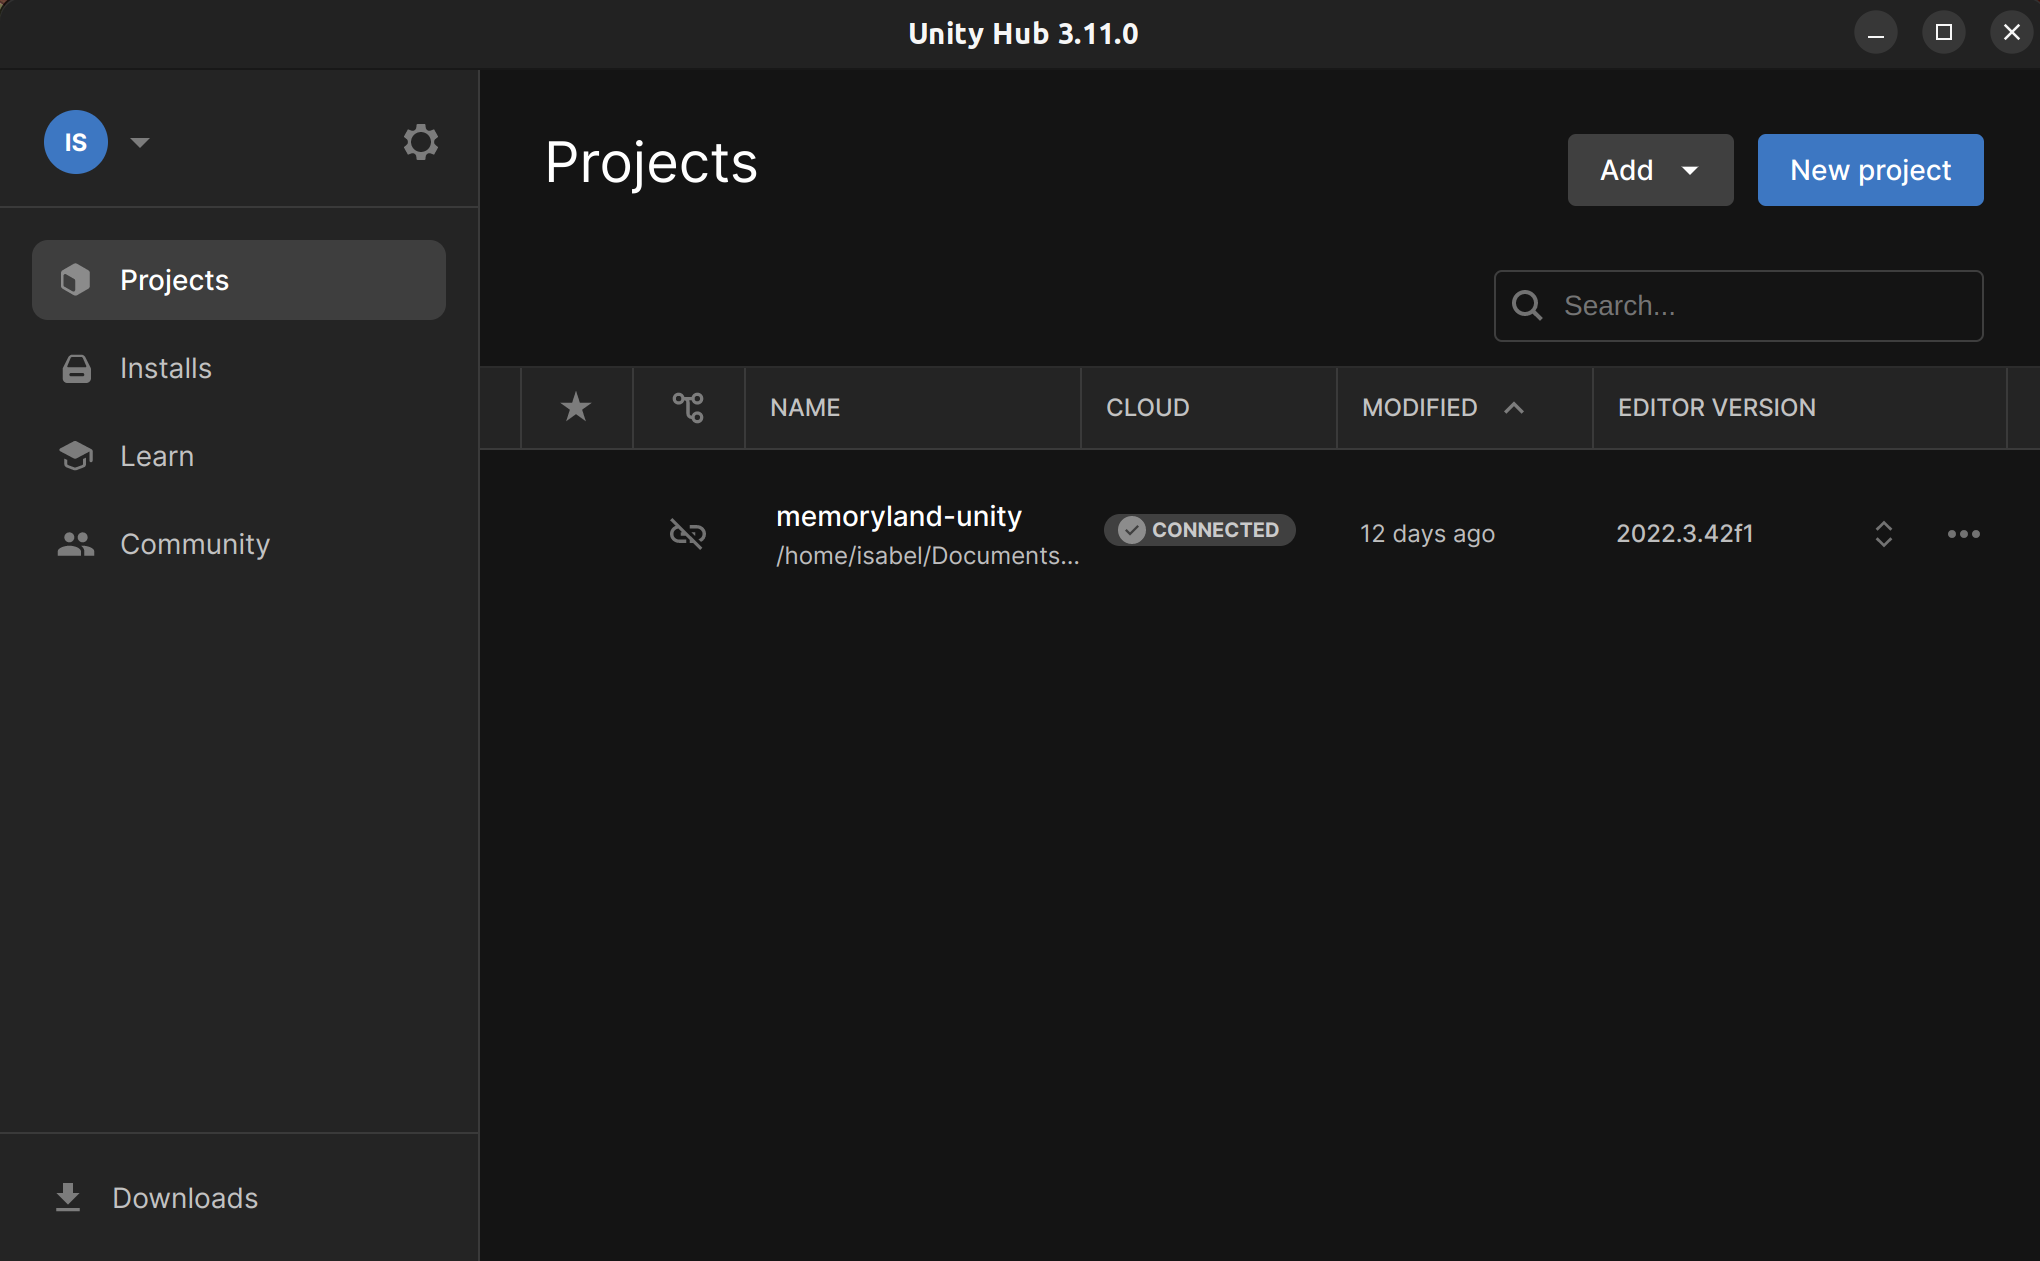
\includegraphics[scale=0.15]{pics/unity-hub.png}
    \caption{Entwicklung in Unity: der Unity-Hub}
    \label{fig:unity-hub}
\end{figure}


Über den \textbf{Unity-Hub} (siehe \ref{fig:unity-hub}) steigt man in den Unity Editor (die IDE, siehe \ref{fig:unity-ide}) ein. Diese Umgebung ist gängigen 3D-Animationsprogrammen und 3D-Entwicklungs-umgebungen nachempfunden. Die Ansicht in der Mitte stellt die aktuelle Sicht auf die Szene dar. Alle gewählten und in der Szene platzierten Objekte befinden sich links in der Hierarchie. Diese wird vor allem für die Auswahl der zu ändernden Objekte verwendet. Auf der rechten Seite befindet sich der Inspektor. Mit seiner Hilfe verändert man einzelne Attribute der sogenannten GameObjects. Es gibt einfach zu ändernde Attribute und veränderliche bzw. durch Programme veränderte Attribute. Die Kombination aus beidem macht Unity so mächtig.\footnote{Alle Infos zum Unity Editor finden sich auch in \cite{UnityDocsEditor}}


\begin{figure} [h t]
    \centering
    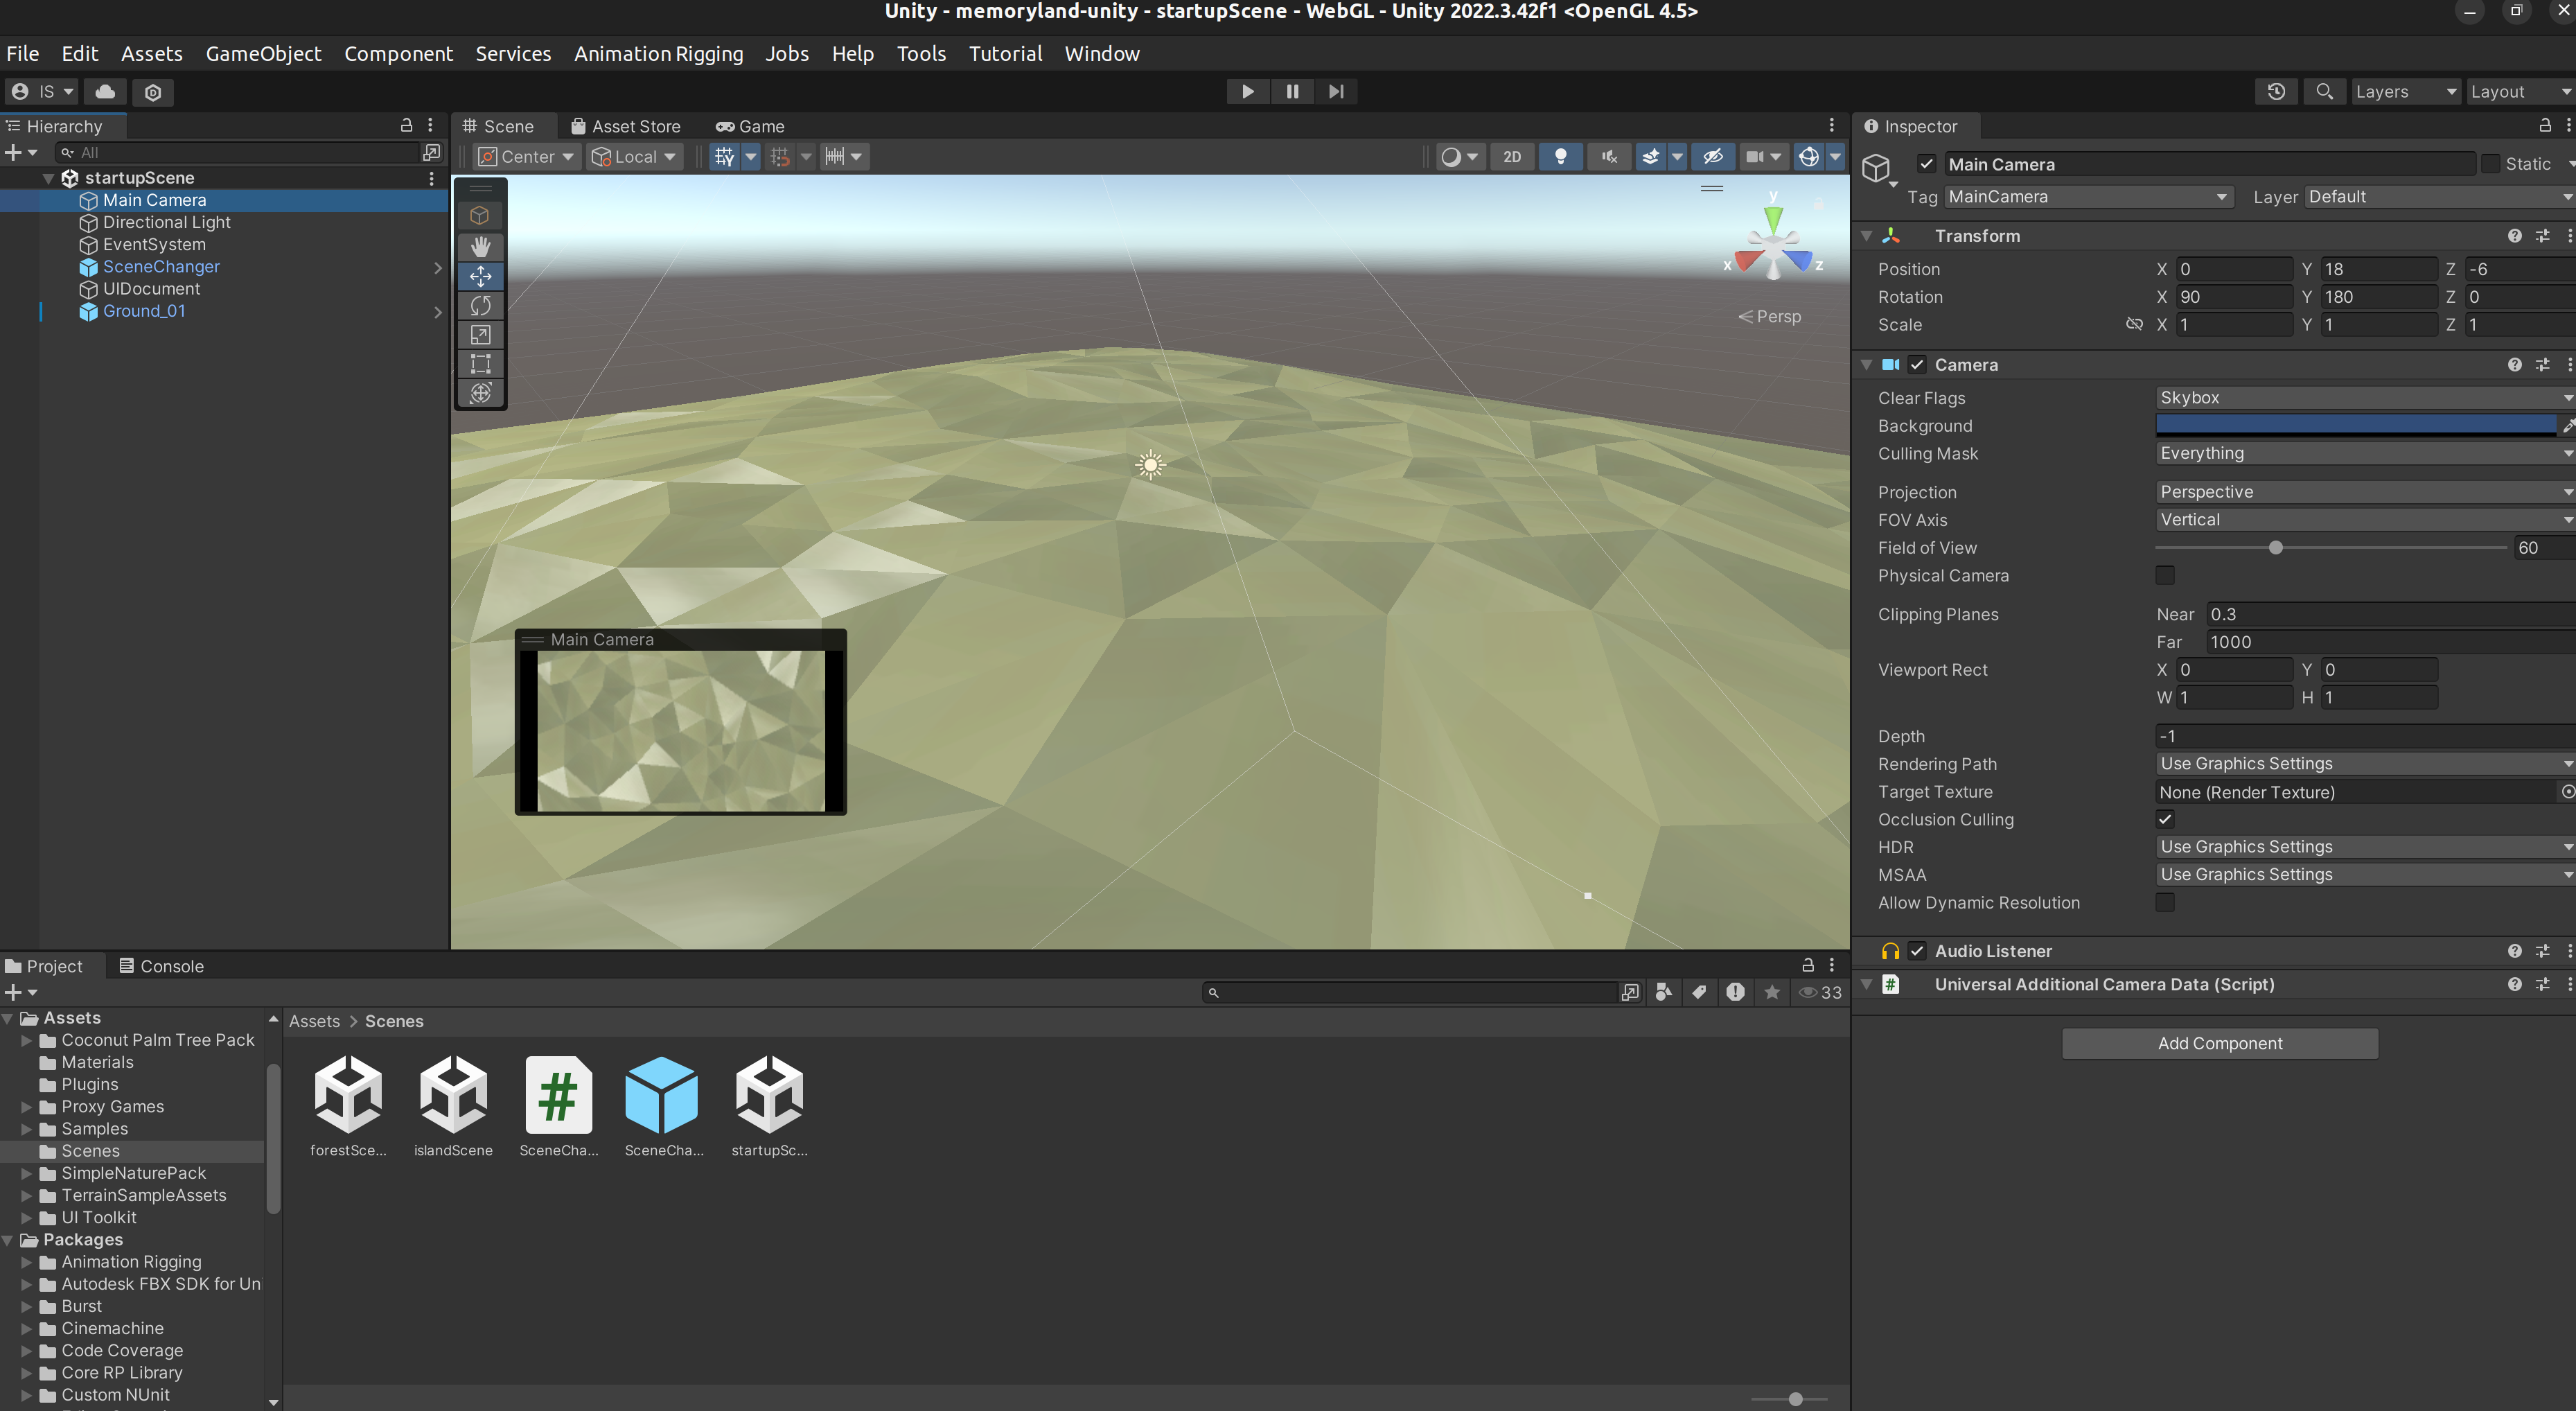
\includegraphics[scale=0.1]{pics/unity-ide.png}
    \caption{Entwicklung in Unity: Die Unity IDE}
    \label{fig:unity-ide}
\end{figure}



Der Entschluss diese Technologie zu verwenden fiel vor allem, weil diese Technologie bereits frühzeitig in unserem Lehrplan enthalten ist und damit umfangreiche Kenntnisse vorhanden waren. Der andere, wesentliche Grund liegt in der \textbf{Erweiterbarkeit} der Umgebung die man in Unity schafft. Die Entwicklungsumgebung ist dergestalt, dass man von Beginn an mit mehreren Scenen im Entwurf gearbeitet hat. Jede Szene (Scene) in Unity spiegelt dabei einen Memorylandtype\footnote{siehe dazu vor allem Abschnitt \ref{sec:memoryland-types}}



\subsection{Visual Studio 2022 und Code}

Der \textbf{Unity Editor} integriert sich mit verschiedenen Source Code Editoren (\Glspl{ide}). Die Entwicklung der entsprechenden Klassen weiter unten erfolgte teils in Windows mit Visual Studio 2022 und später auch unter Ubuntu mit Visual Studio Code und anderen Editoren. Die Editoren unterscheiden sich in der Unterstützung der entsprechenden Intellisense und Syntax-Erkennung. Generell ist aber zu sagen, dass die Entwicklung unter Windows angenehmer ist, da hier die volle Bandbreite einer Umgebung zur Verfügung steht, die einerseits die Bibliotheken kennt und die Syntax prüft.



\section{Unity WebGL}
\label{sec:unity-webgl}

\textbf{Unity} bietet eine besondere Form des Build an: WebGL. \textbf{Unity WebGL} ermöglicht damit die Spiele und interaktiven Anwendungen, die man mit Unity erstellt hat, direkt im Webbrowser aufzurufen, ohne dass zusätzliche Plugins oder Software installiert werden müsste.\footnote{Alle Infos zu Unity WebGL stammen von \cite{UnityDocsWebGL} bzw. \cite{WebGL}}


\begin{wrapfigure}{r}{0.5\textwidth}
    \centering
    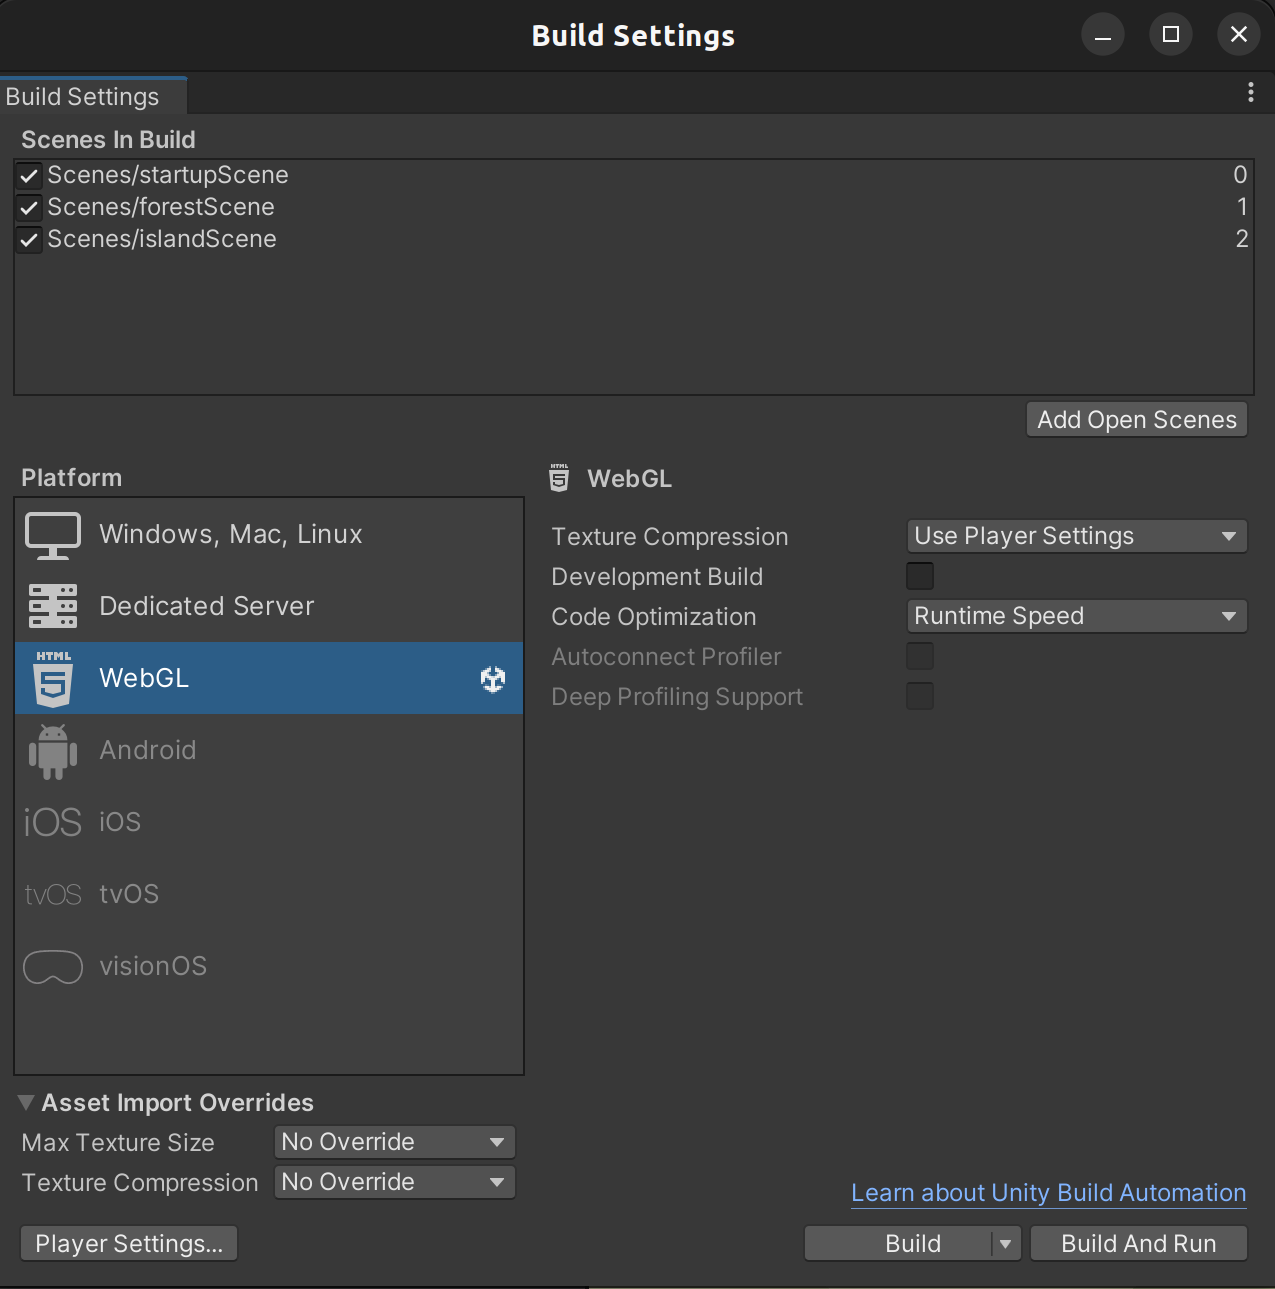
\includegraphics[scale=0.12]{pics/unity-bulid-settings.png}
    \caption{Entwicklung in Unity: Die Unity Build Settings}
    \label{fig:unity-build-settings}

    \vspace{1cm}

    \centering
    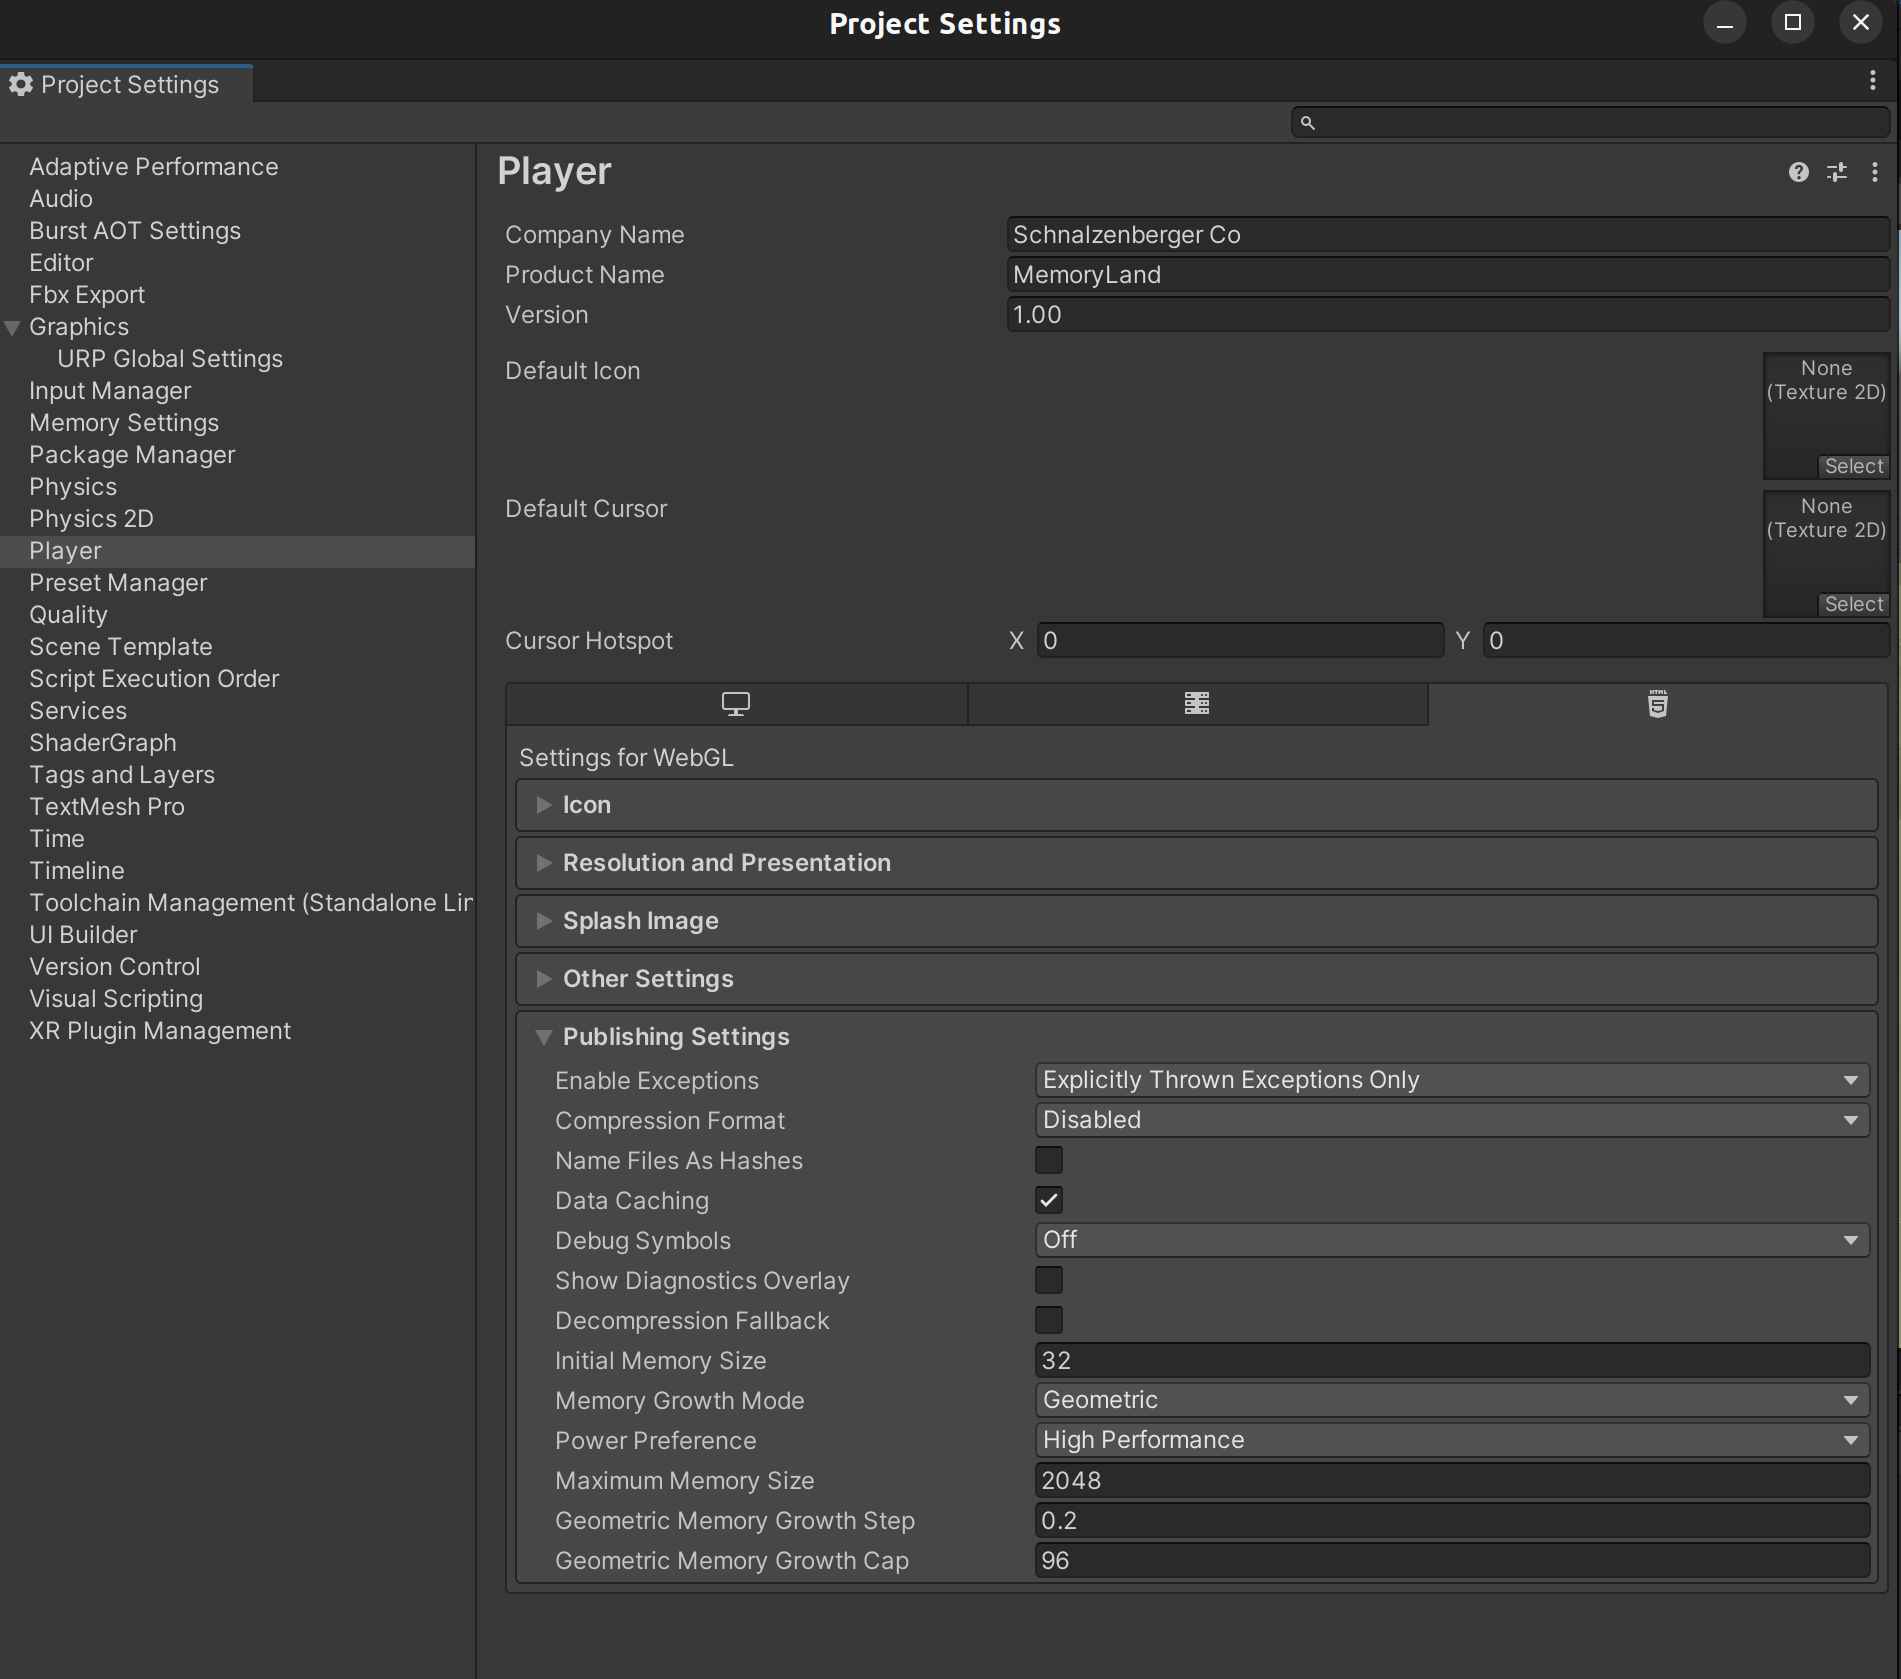
\includegraphics[scale=0.09]{pics/unity-build-webgl-settings.png}
    \caption{Entwicklung in Unity: Die Unity Build Settings für WebGL}
    \label{fig:unity-build-webgl-settings}
\end{wrapfigure}



\textbf{WebGL (Web Graphics Library)} ist eine JavaScript-API, die 3D-Grafiken im Browser rendern kann. Sie basiert dabei auf OpenGL, einer ``shading language'', welche die Beschreibung einer virutellen Umgebung übernimmt. Unity nutzt diese API, um die für Webbrowser optimierte Ausführung von Inhalten zu ermöglichen. WebGL in Unity unterstützt viele gängige Plattformen wie Desktop-Browser (Chrome, Firefox, Safari, etc.) und erlaubt es diesem Projekt die Anwendung Memoryland schnell und einfach online zu verbreiten.


Das Projekt wurde mit den in den Abbildungen \ref{fig:unity-build-settings} und \ref{fig:unity-build-webgl-settings} dargestellten \textbf{Einstellungen} für Unity WebGL entwickelt und der erzeugte JavaScript Code wurde in das Frontend\footnote{im Verzeichnis ``./unity'' siehe Abschnitt \ref{sec:frontend-integration-webgl}} integriert.


Die gewählten Einstellungen entsprechen den Empfehlungen der bereits erwähnten Beschreibungen zu Unity WebGL und insbesondere das ``Data Caching'' wurde eingestellt. Leider funktioniert in diesem Projekt derzeit das gewählte Caching nicht perfekt. Unity WebGL lädt die Datendatei laufend neu und dies ist laut verschiedenen Quellen im Netz derzeit ein Fehler in der gewählten Umgebung, der in naher Zukunft behoben werden soll.\footnote{Hauptquellen: \cite{UnityDocsDataCachingIssue} und \cite{UnityDocsDataCachingIssue2}}


\section{Implementierung des Unity Projekts}

Die Entwicklung des Unity Projektes ist der grö\ss{}




\subsection{Url-Parameter}
\label{subsec:unity-url-parameter}

Es ist notwendig \emph{Daten vom Frontend mit Unity} auszutauschen. Es gibt derzeit viele entsprechende Mechanismen. Die gewählte \textbf{Methode über URL-Parameter} vermeidet Verschränkungen zwischen der Implementierung des Frontend (und dessen Services in Richtung Backend) und der Implementierung von den Szenen in Unity.


Für den gewählten Prozess der \emph{Übergabe der Parameter} über den IFrame mit Hilfe von herkömmlichen URL-Parametern (siehe Listing \ref{lst:unity-url-parameter-in-action}) gab es bereits mehrere Realisierungen und Erfahrungsberichte. Diese verwendeten alle eine Form der Verschränkung von JavaScript Code mit Unity C\# Code. 



\begin{lstlisting}[numbers=left,caption={IFrame for Unity in Frontend},label={lst:unity-url-parameter-in-action}]
this.safeUrl = this.sanitizer
          .bypassSecurityTrustResourceUrl(`/unity/index.html?token=${myToken}& server=${environment.apiConfig.uri}`);
\end{lstlisting}


Es wurde eine fortgeschrittene Entwicklung einer \textbf{UrlParameter}-Klasse aus dem Projekt übernommen und erweitert.\footnote{Der Originalcode wurde von \cite{UrlParameter} übernommen und um eine weitere Funktion erweitert.} Die enthaltenen Funktionen sahen nur nummerische Parameter vor und so war die gewählte Übergabe eines GUID-Token aus dem Frontend vorerst nicht möglich. Die Funktion ``GetString'' (siehe Listing \ref{lst:unity-url-parameter}) wurde daher in die Klasse \textbf{``DictionaryStringStringExt''} eingefügt. Es waren ansonsten keine weiteren Änderungen notwendig.

Das vorhandene \textbf{Singleton-Skript} ermöglicht einen \textbf{einfachen Zugriff} auf alle URL-Parameter und -Komponenten in einer WebGL-Build-Anwendung. Es muss hierzu eine jslib-Datei verwendet werden, die den JavaScript-Teil aktiviert. Dieses Skript wird beim Importieren in ein Projekt automatisch eine jslib-Datei in den Plugins-Ordner extrahieren, die den Namen „URLParameters.jslib“ trägt.

Um auf die verschiedenen URI-Teile zuzugreifen, kann man einfach die statischen Methoden dieser Klasse verwenden. Die verfügbaren Eigenschaften sind Protocol, Hostname, Port, Pathname, Search, Hash sowie Host, Origin und Href. Damit kann man mithilfe der Funktion \textbf{``URLParameters.GetSearchParameters()''} an beliebiger Stelle in Unity ein Dictionary mit den Url-Parametern laden.

\begin{lstlisting}[numbers=left,caption={UrlParameter},label={lst:unity-url-parameter}]
public static class DictionaryStringStringExt
{
    public static double GetDouble(this Dictionary<string, string> aDict, string aKey, double aDefault)
    {
        string str;
        if (!aDict.TryGetValue(aKey, out str))
            return aDefault;
        double val;
        if (!double.TryParse(str, NumberStyles.Float, CultureInfo.InvariantCulture, out val))
            return aDefault;
        return val;
    }
    public static int GetInt(this Dictionary<string, string> aDict, string aKey, int aDefault)
    {
        string str;
        if (!aDict.TryGetValue(aKey, out str))
            return aDefault;
        int val;
        if (!int.TryParse(str, NumberStyles.Integer, CultureInfo.InvariantCulture, out val))
            return aDefault;
        return val;
    }
    public static string GetString(this Dictionary<string, string> aDict, string aKey, string aDefault)
    {
        string str;
        if (!aDict.TryGetValue(aKey, out str))
            return aDefault;
        return str;
    }
}
\end{lstlisting}


\subsection{Die Startup Szene}
\label{subsec:unity-startup-scene}


\begin{figure} [h t]
    \centering
    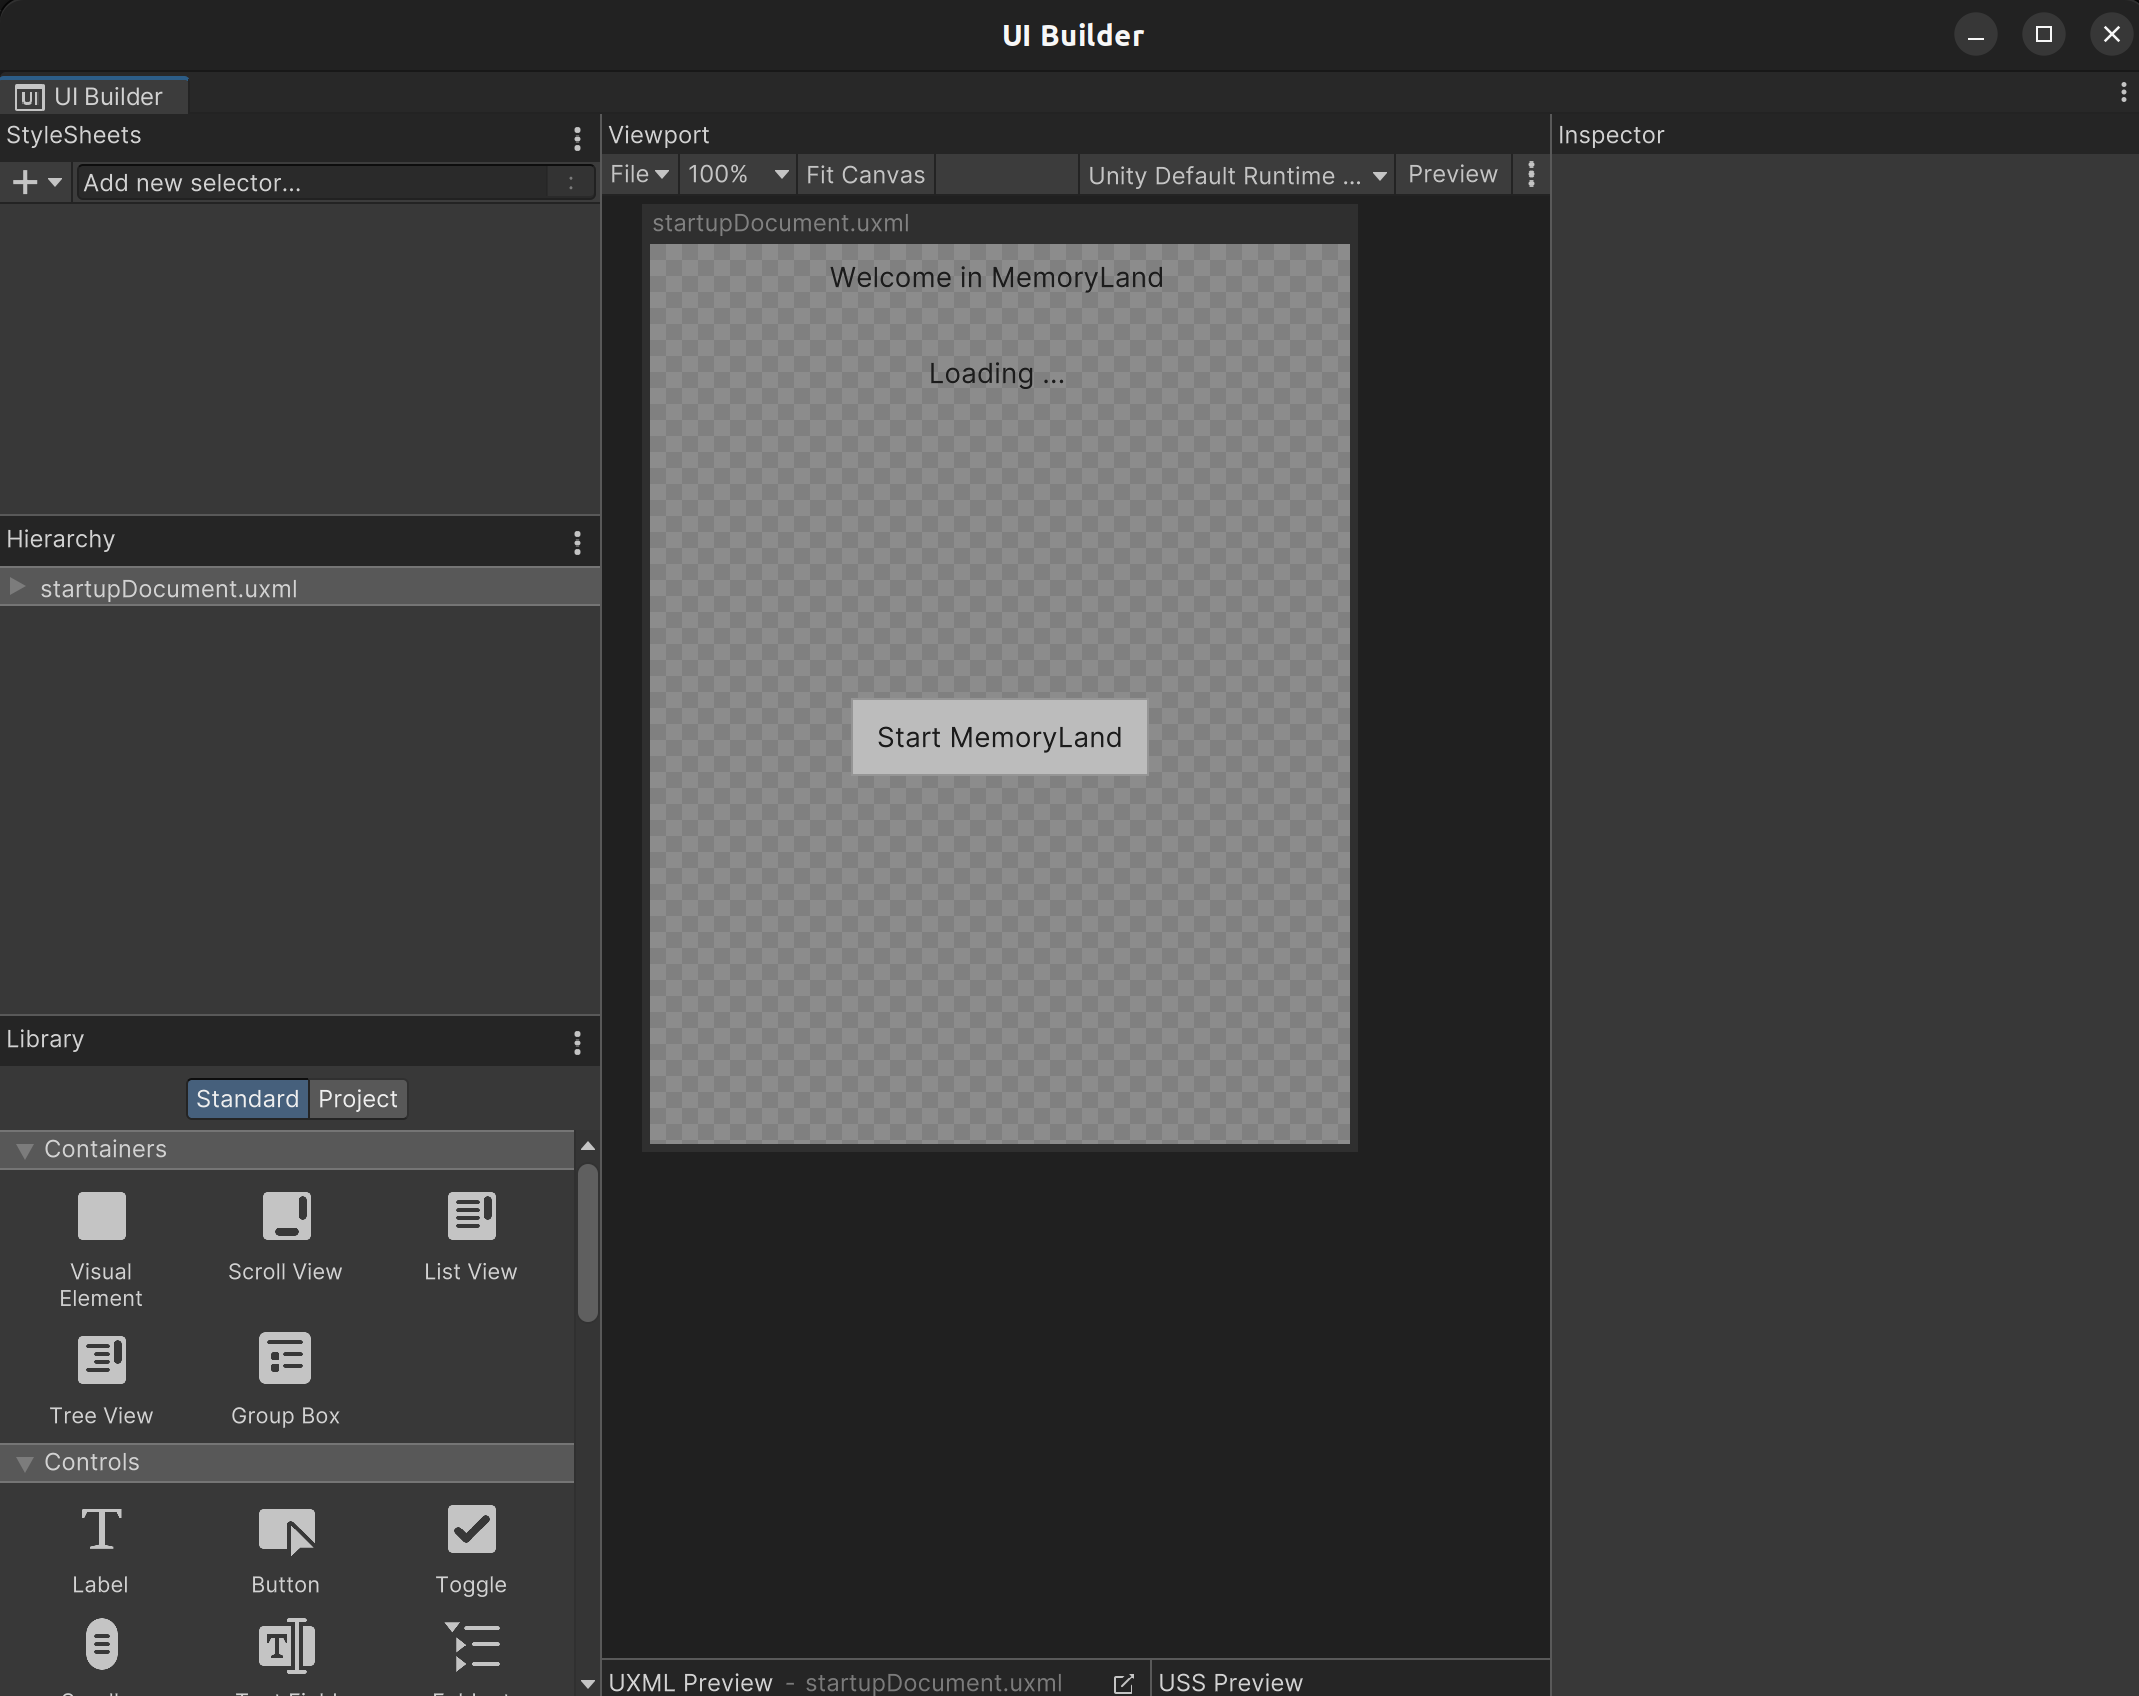
\includegraphics[scale=0.12]{pics/unity-ui-builder.png}
    \caption{Entwicklung in Unity: Der Unity UI Toolkit}
    \label{fig:unity-ui-builder}
\end{figure}


Die Szene ist bereits in Abbildung \ref{fig:unity-ide} zu sehen. Es wurde ein \textbf{leeres Terrain} gebaut und eine \textbf{Unity UI} darübergelegt.\footnote{Die dazu verwendete Technologie Unity UI Toolkit ist in \cite{UnityDocsUIToolkit} beschrieben.} Diese UI dient dazu den Nutzer zu informieren, dass nun die Bilder und die Szene geladen werden. Im Listing \ref{lst:unity-startup-document} sind die wesentlichen Codeteile enthalten. Die Methode \textbf{``OnEnable''} wird aufgerufen, wenn die Startup-Szene die UI aufruft, also zu Beginn des Memoryland. Es werden die UI Komponenten in die Membervariablen geladen und danach sofort die asynchrone Routine zur Überwachung der Fotobeladung im \textbf{``SceneChanger''} gestartet. 


Die Während der ``SceneChanger'' (siehe Listing \ref{lst:unity-scene-changer-start}) die Beladung der Texturen betreibt, wartet der \textbf{``StartupDocument''-UI} bereit darauf, dass es diese Aufgabe abschlie\ss{}t. Diese Information wird mittels der asynchronen Funktion \textbf{``isValid''} (siehe Listing \ref{lst:unity-scene-changer-public}) überprüft. Sobald die Daten und Fotos geladen sind, steht dort der Szenenname zur Verfügung. Falls nun die Szene bekannt ist (derzeit nur ``forest'' oder ``island''), kann die Szene gestartet werden, ansosnten wird der Benutzer mittels des Informationsfeldes darauf hingewiesen, dass ein Fehler aufgetreten ist.



\begin{lstlisting}[numbers=left,caption={StartupDocument für Unity UI Toolkit},label={lst:unity-startup-document}]
....    
    public class StartupDocument : MonoBehaviour
    {
        private Button _start;
        private Label _loading;
        private string chosenScene = null;
           
        //Add logic that interacts with the UI controls in the `OnEnable` methods
        private void OnEnable()
        {
            // The UXML is already instantiated by the UIDocument component
            var uiDocument = GetComponent<UIDocument>();
    
            _start = uiDocument.rootVisualElement.Q("start") as Button;
            _start.SetEnabled(false);
            _loading = uiDocument.rootVisualElement.Q("loading") as Label;
            _start.RegisterCallback<ClickEvent>(PrintClickMessage);
            
            StartCoroutine(LoadFromLikeCoroutine());
        }
    
        private IEnumerator LoadFromLikeCoroutine()
        {
            while (chosenScene == null) {
            IEnumerator tgt = FindAnyObjectByType<SceneChanger>().IsValid();
            while (tgt.MoveNext()) 
            {
                chosenScene = (string)tgt.Current;
                yield return chosenScene;
            }
            }
            
            if (chosenScene != "ERROR") {
                Debug.Log("Finished!");
                _loading.text = "Finished Loading " + chosenScene;
                _start.SetEnabled(true);
                FindAnyObjectByType<SceneChanger>().StartThisNow();
            }
            else 
            {
                _loading.text = "Sorry, ERROR Loading this Memoryland. Possibly Token invalid!";
                Debug.Log("ERROR loading");
            }
        }
        ....
    }        
\end{lstlisting}


Die Klasse \textbf{``SceneChanger''} existiert länger im Projekt. Zu Beginn hatte sie nur die Aufgabe den Szenenwechsel bereitzustellen, inzwischen hat sich das Aufgabengebiet auf das Laden aller Bestandteile der Szenen ausgeweitet. Sie hat daher drei Aufgaben: das \textbf{Laden der Memoryland-Informationen} aus dem Backend, die Beladung der Texturenliste (also der \textbf{Fotos}) und die Bereitstellung einer \textbf{Szenen-Wechsel-Funktion}.

Die Funktion \textbf{``Start''} lädt die URL-Parameter mit Hilfe der Klasse aus Abschnitt \ref{subsec:unity-url-parameter} in die enstprechenden statischen Membervariablen. Zu Testzwecken wurde ein ``fallbackResponse'' und ein dazugehöriger Parameter (``fallback'' == ``yes'') eingeführt, sodass Szenen zeitnah und während der Implementierung mit echten Bildern aus dem Backend getestet werden können.

Nach der Beladung der Variablen werden diese verwendet, um die URL zum \textbf{Aufruf des REST Backend} mit dem Token\footnote{siehe dazu vor allem auch die Abschnitts \ref{backend-memoryland-controller} und \ref{subsec:frontend-explore-worlds}} zusammenzusetzen. Die Verwendung des Token ermöglicht den Aufruf der Memorylands auch durch nicht-eingeloggte Benutzer.



\begin{lstlisting}[numbers=left,caption={SceneChanger - Start},label={lst:unity-scene-changer-start}]
        ....
        
        public class SceneChanger : MonoBehaviour
        {
        
            private static 
                string fallbackResponse = @"
                ....
                ";
        
            private static string chosenScene = null;
            private static string token = null;
            private static string server = "https://app-memoryland.azurewebsites.net";
            private static string fallback = "no";
            private static Dictionary<int, string> allUrls = null;
        
            private static Dictionary<int, Texture> allTextures = new Dictionary<int, Texture> ();
        
            ....                
        
            // Start is called before the first frame update
            IEnumerator Start()
            {
                // already loaded?
                if (SceneChanger.token == null && SceneChanger.chosenScene == null) 
                {
                    // first load the given token
                    Dictionary<string,string> paras =  URLParameters.GetSearchParameters();
                    SceneChanger.token = paras.GetString("token", "");
                    SceneChanger.server = paras.GetString("server", "https://app-memoryland.azurewebsites.net");
                    
                    if (Application.platform == RuntimePlatform.WebGLPlayer)
                    {
                        SceneChanger.fallback = paras.GetString("fallback", "no");
                    }
                    else
                    {
                        SceneChanger.fallback = paras.GetString("fallback", "no");
                        SceneChanger.token = paras.GetString("token", "1920cf9e-b295-4c80-b347-75eff21a71f6");
                    }
                    
                    Debug.Log("Parameter Value token = " + SceneChanger.token);
                    Debug.Log("Parameter Value server = " + SceneChanger.server);
                    Debug.Log("Parameter Value fallback = " + SceneChanger.fallback);
                    
                    if (SceneChanger.fallback == "yes")
                    {
                        yield return SetInternals(SceneChanger.fallbackResponse);
                        Debug.LogError("Fallback is set => Using simulation init parameters to start with!");
                    }
                    else
                    {
                        // missing call to the url/backend
                        string uri = SceneChanger.server+"/api/Memoryland?token=" + SceneChanger.token;
                        string response = "";
                        
                        using (UnityWebRequest webRequest = UnityWebRequest.Get(uri))
                        {
                            yield return webRequest.SendWebRequest();
                        
                            switch (webRequest.result)
                            {
                            case UnityWebRequest.Result.ConnectionError:
                            case UnityWebRequest.Result.DataProcessingError:
                                Debug.LogError(SceneChanger.server + ": Error: " + webRequest.error);
                                    SceneChanger.chosenScene = "ERROR";
                                break;
                            case UnityWebRequest.Result.ProtocolError:
                                Debug.LogError(SceneChanger.server + ": HTTP Error: " + webRequest.error);
                                    SceneChanger.chosenScene = "ERROR";
                                break;
                            case UnityWebRequest.Result.Success:
                                Debug.Log(SceneChanger.server + ": Received: " + webRequest.downloadHandler.text);
                                response = webRequest.downloadHandler.text;
                                yield return SetInternals(response);
                                break;
                            default:
                                Debug.LogError(SceneChanger.server + ": unknown " + webRequest.result.ToString());
                                    SceneChanger.chosenScene = "ERROR";
                                break;
                            }
                            }
                        }
                }		
            }
        ....
        }
\end{lstlisting}
    

Das Umwandeln des gelieferten JSON im Textformat übernimmt dann die Funktion \textbf{``SetInternals''}. Es wurden einige serialisierbare Basisklassen für die im JSON enthaltenen Daten erstellt. Diese sind ``MemorylandType'', ``MemorylandConfiguration'' und ``Memoryland''. Die Funktion nimmt den gelieferten String und verwendet die Unity-Basisklasse \textbf{``JsonUtility''} um diesen zu C\# Objekten zu konvertieren.

Danach wird sofort für jede gelieferte Foto-URL die asynchrone Funktion \textbf{``LoadTexture''} aufgerufen. Dies ermöglicht ein möglichst rasches Laden der Bilder bei einem verzerrungs- und störungsfreien Ansehen des Memorylands bzw. der entsprechenden Szene. 

\begin{lstlisting}[numbers=left,caption={SceneChanger - SetInternals},label={lst:unity-scene-changer-set-internals}]
    ....   
    
        [System.Serializable]
        public class MemorylandType
        {
            public string name;
            public int photoAmount;
        }
        
        [System.Serializable]
        public class MemorylandConfiguration
        {
            public int position;
            public string photo;
        }
        
        
        [System.Serializable]
        public class Memoryland
        {
            public long id;
            public string name;
            public MemorylandType memorylandType;
            public List<MemorylandConfiguration> memorylandConfigurations;
        
            public static Memoryland CreateFromJSON(string jsonString)
            {
                return JsonUtility.FromJson<Memoryland>(jsonString);
            }
        }
    ....
    private IEnumerator SetInternals(string response) 
    {
        Debug.Log("setInternals now with ");
        if (response != null) {
        
            Memoryland ml = null;
            try {
                ml = Memoryland.CreateFromJSON(response);
            }
            catch (Exception e)
            {
                Debug.LogError("Error Reading response! " + e.ToString());
            }
            
            if (ml != null) 
            {
                if (ml.memorylandConfigurations != null) {
                    SceneChanger.allUrls = new Dictionary<int, string>();
                    foreach (MemorylandConfiguration item in ml.memorylandConfigurations) {
                        Debug.Log("got one photo " + item.position.ToString());
                        SceneChanger.allUrls[item.position] = item.photo;
                        yield return LoadTexture(item.position, item.photo);
                    }
                }

                // always set the pics first
                if (ml.memorylandType != null && ml.memorylandType.name != null ) {
                    SceneChanger.chosenScene = ml.memorylandType.name;
                    Debug.Log("Got Scene from response: " + chosenScene);
                }
            }
        }
        
        if (SceneChanger.allUrls == null) 
        {
            SceneChanger.chosenScene = "ERROR";
            Debug.LogError("no URLs loaded!");
        }
    }    
\end{lstlisting}
    
Die Bilder bzw. Fotos werden vom Backend in Form von URLs mit SAS-Tokens (mit beschränkter Gültigkeit\footnote{siehe dazu vor allem Abschnitt \ref{subsection:sas-token-generation}}) beim Call gegen das REST Backend geliefert. Diese Bilder werden sofort als Texturen in den Speicher geladen um Verzögerungen und fehlende Darstellungen zu vermeiden. Dies übernimmt die in Listing \ref{lst:unity-scene-changer-load-texture} enthaltene Funktion \textbf{``LoadTexture''}. Es wird dazu - wie oben für den Call ins Backend - die Unity Basisklasse \textbf{``UnityWebRequest''} verwendet.


\begin{lstlisting}[numbers=left,caption={SceneChanger - LoadTexture},label={lst:unity-scene-changer-load-texture}]
  
    IEnumerator LoadTexture (int id, string uri)
    {
        Debug.Log("Load Photo " + id.ToString() + " with " + uri);
        Texture myTexture = null;
        using (UnityWebRequest imageRequest = UnityWebRequestTexture.GetTexture(uri))
        {
            yield return imageRequest.SendWebRequest();
            
            switch (imageRequest.result)
            {
            case UnityWebRequest.Result.ConnectionError:
            case UnityWebRequest.Result.DataProcessingError:
                Debug.LogError("Photo Error: " + imageRequest.error);
                break;
            case UnityWebRequest.Result.ProtocolError:
                Debug.LogError("Photo HTTP Error: " + imageRequest.error);
                break;
            case UnityWebRequest.Result.Success:
                Debug.Log("Received Photo " + id.ToString() + " with " + uri);
                //
                myTexture = DownloadHandlerTexture.GetContent(imageRequest);
                SceneChanger.allTextures[id] = myTexture;
                break;
            default:
                Debug.LogError("Photo unknown result: " + imageRequest.result.ToString());
                break;
            }	    
        }
            yield return "Loaded";
    }
\end{lstlisting}
    

Schlussendlich bleibt die letzte Funktion des SceneChanger, welche schon von Beginn bestanden hatte: der Szenenwechsel mithilfe von \textbf{``StartThisNow''}. Sie wird mit Hilfe der Standard-Unity Funktionalität von SceneManager abgebildet. Es wird zusätzlich überprüft, ob diese Szene überhaupt im WebGL Build existiert.\footnote{Die Build-Settings von WebGL können der Abbildung \ref{fig:unity-build-settings} entnommen werden. Dort steht auch eine Liste der enthaltenen Szenen.} Die weiteren Funktionen \textbf{``isValid'' und ``GetOneTexture''} werden von anderen Klassen verwendet um die aktuelle Szene bzw. einzelne Fotos (bereits als Texturen) abzurufen.


\begin{lstlisting}[numbers=left,caption={SceneChanger},label={lst:unity-scene-changer-public}]
....
    public class SceneChanger : MonoBehaviour
    {
        ....
        
        private void ChangeScene(string sceneName)
        {
            if (SceneManager.GetActiveScene().name == sceneName + "Scene" || (sceneName == "ERROR"))
            {
                Debug.Log("Scene " + sceneName + " already active!");
            }
            else 
            {
                Debug.Log("Change Scene to " + sceneName);
                SceneManager.LoadScene (sceneName + "Scene");
            }
        }
        ....
        public IEnumerator GetOneTexture(int position)
        {
            if (SceneChanger.allUrls == null || SceneChanger.chosenScene == null) // not finished call to backend
                yield return null;
                
            if (SceneChanger.allTextures.ContainsKey(position)) {
                yield return SceneChanger.allTextures[position];
            }
            else 
            {
                Debug.Log(position.ToString() + " NOT FOUND in MemoryLand!");
                yield return null;
            }
        }
    
        ....    
        public IEnumerator IsValid()
        {
            if (SceneChanger.chosenScene == null) // not finished call to backend
                yield return null;
                
            yield return (SceneChanger.chosenScene);
        }
    
        public void StartThisNow()
        {
            // now change scene
            ChangeScene(SceneChanger.chosenScene);
        }
    
        ....
    }
\end{lstlisting}

\subsection{Einfügen von Images}
\label{subsec:unity-image-loader}

Am Beginn des Projektes wurden die Fotos als Texturen vom Backend erst nach dem Start der Szene geladen, also in Form eines Lazy-Load während die Szene bereits abläuft. Dies führte dazu, dass die ersten Fotos noch nicht fertig geladen waren und die Planes noch im Platzhalter-Modus (hier wurde eine blaue Farbe für das Plane gewählt) dargestellt wurden. Dieses Vorgehen war äußerst unpassend für das angestrebte Nutzererlebnis. 

Das Laden der Fotos wurden daher im Rahmen einem weiteren Sprint im Code zeitlich vorverlegt und findet nun während des Startup in der Startup-Szene statt. Dazu wird der Nutzer im Rahmen der Startup-Szene (siehe Abschnitt \ref{subsec:unity-startup-scene}) im gewählten UI über den Ladeprozessfortschritt informiert.

Der hier beschriebene \textbf{``ImageLoader''} hat damit nur noch die Aufgabe die entsprechende Texture vom \textbf{``SceneChanger''} (siehe Abschnitt \ref{subsec:unity-startup-scene}) zu laden und dann das Format des Plane anzupassen. Die Bilder würden ansonsten verzerrt angezeigt. Dazu wird mit Hilfe eines \textbf{``Vector3''} Objekts die Größe und damit Verzerrung des Planes eingestellt. Aufrecht stehende Bilder können in Unity nicht gedreht werden (EXIF-Informationen werden ignoriert), daher musste dies bereits vom Backend übernommen werden.\footnote{siehe hierzu vor allem Abschnitt \ref{subsec:backend-rotate-pictures}} 


\begin{lstlisting}[numbers=left,caption={ImageLoader},label={lst:unity-image-loader}]
....
public class ImageLoader : MonoBehaviour
{
    public int urlID = 0;
    public Renderer thisRenderer;

    // Start is called before the first frame update
    void Start()
    {
        // the following will be called even before the load finished
        thisRenderer.material.color = Color.blue;

        StartCoroutine(LoadFromLikeCoroutine()); // execute the section independently
    }

....

    // this section will be run independently
    private IEnumerator LoadFromLikeCoroutine()
    {
	Texture myTexture = null;
	
        IEnumerator tgt = FindAnyObjectByType<SceneChanger>().GetOneTexture(urlID);
        while (tgt.MoveNext()) 
        {
        	myTexture = (Texture)tgt.Current;
        	yield return myTexture;
        }
        
        if (myTexture == null) {
        	yield return null;
        }

	if (myTexture == null) {
            	thisRenderer.material.color = Color.red;          // set red
		Debug.Log("Image NotFound!");
		yield return null;
	}
	else 
	{
		Debug.Log("Loaded");
		thisRenderer.material.color = Color.white;          // set white

		float scale = 0.3f;

		//thisRenderer.gameObject.
		if (myTexture.height > myTexture.width)
		{
			float f = (float)myTexture.height / (float)myTexture.width * scale;
			thisRenderer.transform.localScale = new Vector3(scale, scale, f);
			//thisRenderer.material.SetTextureScale("_MainTex", new Vector2(1f, 0.5f));

		}
		else
		{
			//float f = ((float)myTexture.width * (float)0.5) / ((float)myTexture.height * (float)0.5);
			float f = (float)myTexture.width / (float)myTexture.height * scale;
			thisRenderer.transform.localScale = new Vector3(f, scale, scale);
			//thisRenderer.material.SetTextureScale("_MainTex", new Vector2(0.5f, 1f));

		}

		thisRenderer.material.mainTexture = myTexture ;  // set loaded image
	}
    }
}
\end{lstlisting}




\section{Erstellung von Szenen bzw. Memoryland-Typen}

Das Projekt enthält bereits zwei vordefinierte Szenen:

\begin{itemize}
    \item Die \textbf{Wald-Szene} (MemorylandType == ``forest'') mit 10 Bildern
    \item Die \textbf{Insel-Szene} (MemorylandType == ``island'') mit 10 Bildern
\end{itemize}


\subsection{Der Dolly Track}
\label{subsec:unity-dolly-track}

..... \emph{OFFEN} WEITER, TODO





\subsection{Die Wald-Szene}

Die Erstellung der Wald-Szene war am schwierigsten, da die ersten Entwürfe und die Ideenfindung über diese Szene erfolgte. Es wurde versucht einerseits eine \textbf{ansprechende und umfangreiche Waldumgebung} zu erzeugen. Die Idee, die hinter einer Waldumgebung stand, ist die Darstellung von Fotos und Erinnerungen aus einer Wanderung im Grünen.



\begin{figure} [h t]
    \centering
    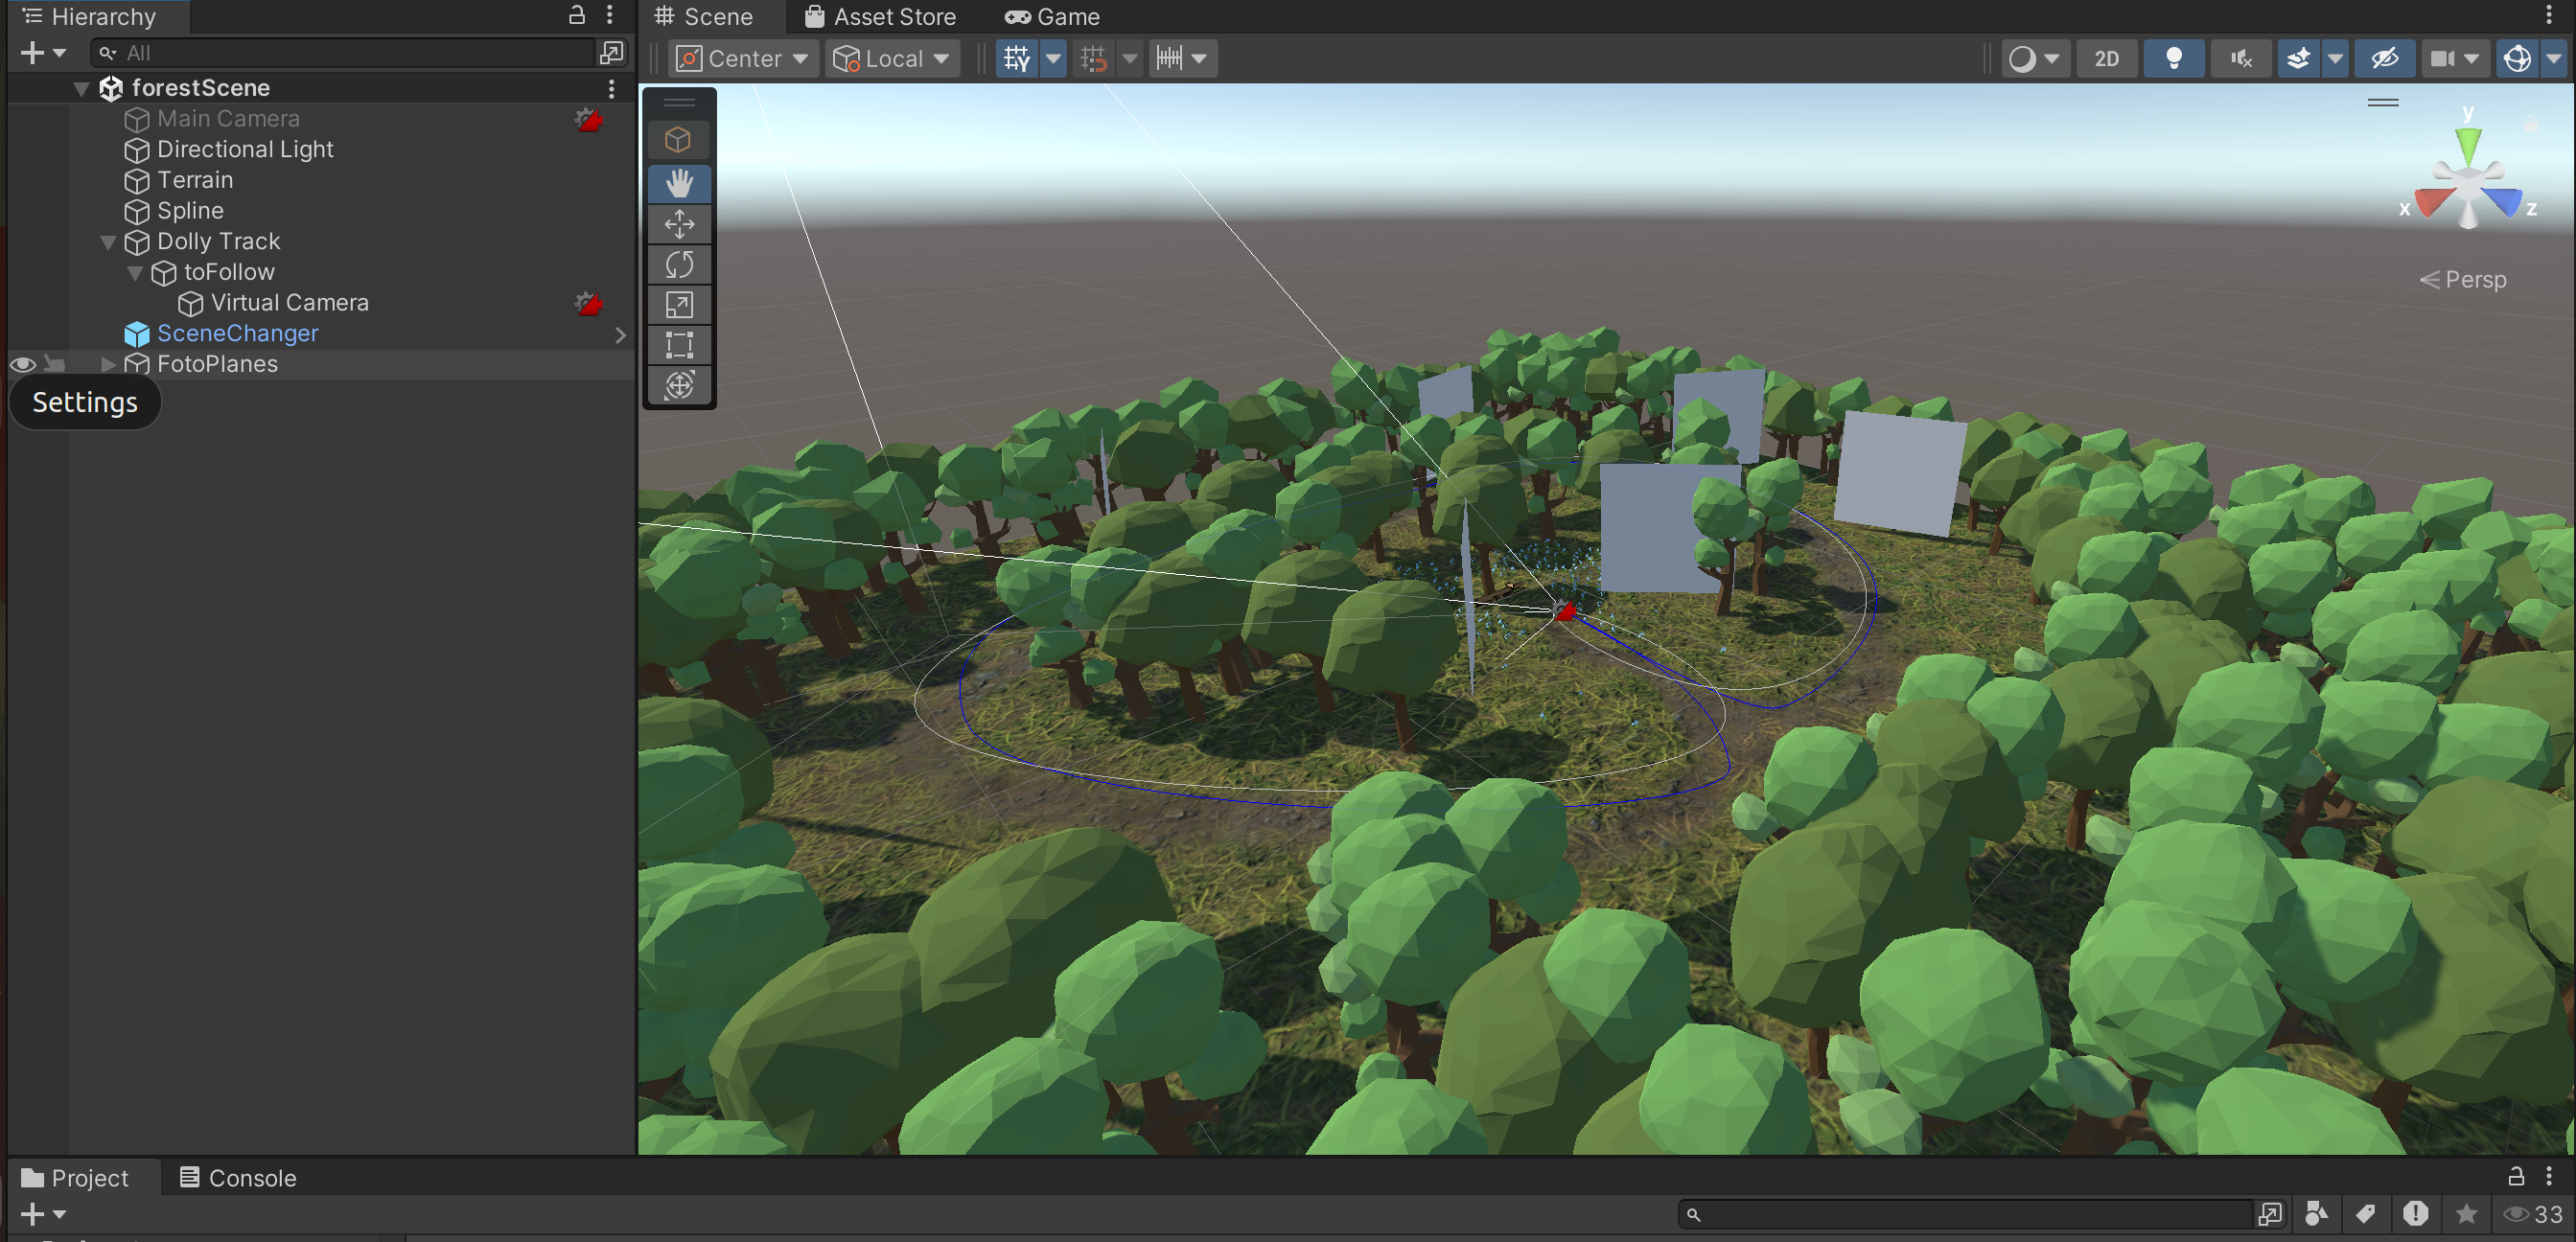
\includegraphics[scale=0.15]{pics/unity-edit-forest.png}
    \caption{Entwicklung in Unity: Die Wald Szene}
    \label{fig:unity-edit-forest}
\end{figure}


Diese \textbf{Wanderungserinnerung} ließ sich für die Autoren am klarsten durch einen Wald abrufen. Ein Wald mit vielen verschiedenen Bäumen und Blumen. Die Szene wurde also entsprechend aufgebaut. Dabei wurde zuerst teilweise auf Beispiele aus dem Unterricht zurückgegriffen. Diese waren aber leider \textbf{zu detailreich}, um auch wirklich auf allen Zielplattformen dargestellt werden zu können. Die Anzahl der Details wurde daher reduziert.

Die Wanderung selbst wird durch die Verwendung des Konzepts des \textbf{Dolly Track} (siehe Abschnitt \ref{subsec:unity-dolly-track}) durchgeführt. Die Nutzer erleben einen Waldspaziergang mit Bäumen und Blumen, während sie an den Bildern vorüberschreiten.


\subsection{Die Insel-Szene}

Nachdem die umfangreichen Tests der Integration der Unity WebGL in das Frontend und das laufende Backend erfolgreich waren, stand nun der Weg offen für die Entwicklung einer \textbf{weiteren Ferien-Umgebungs-Szene}. Die \textbf{Insel-Szene} war mit dem Erlebnis einer \textbf{sandigen Insel mit Sonne, Strand und Meer bei Sonnenuntergang} für die Entwickler die logischste Wahl.   

Mehrere Palmen (``Palm Trees'') und Steine wurden auf der Insel in verschiedenen Winkeln und Punkten so platziert, dass der Eindruck einer Südseeinsel entsteht. Die Sonne wurde so platziert, dass es sich um einen Sonnenauf- bzw. -untergang handeln könnte. Einige kleinere Elemente, wie bspw. dürre Gräser wurden in der nähe des Meeres platziert. Das Meer selbst ist auch ein umfangreiches Prefab namens ``Detailed Water''. 



\begin{figure} [h t]
    \centering
    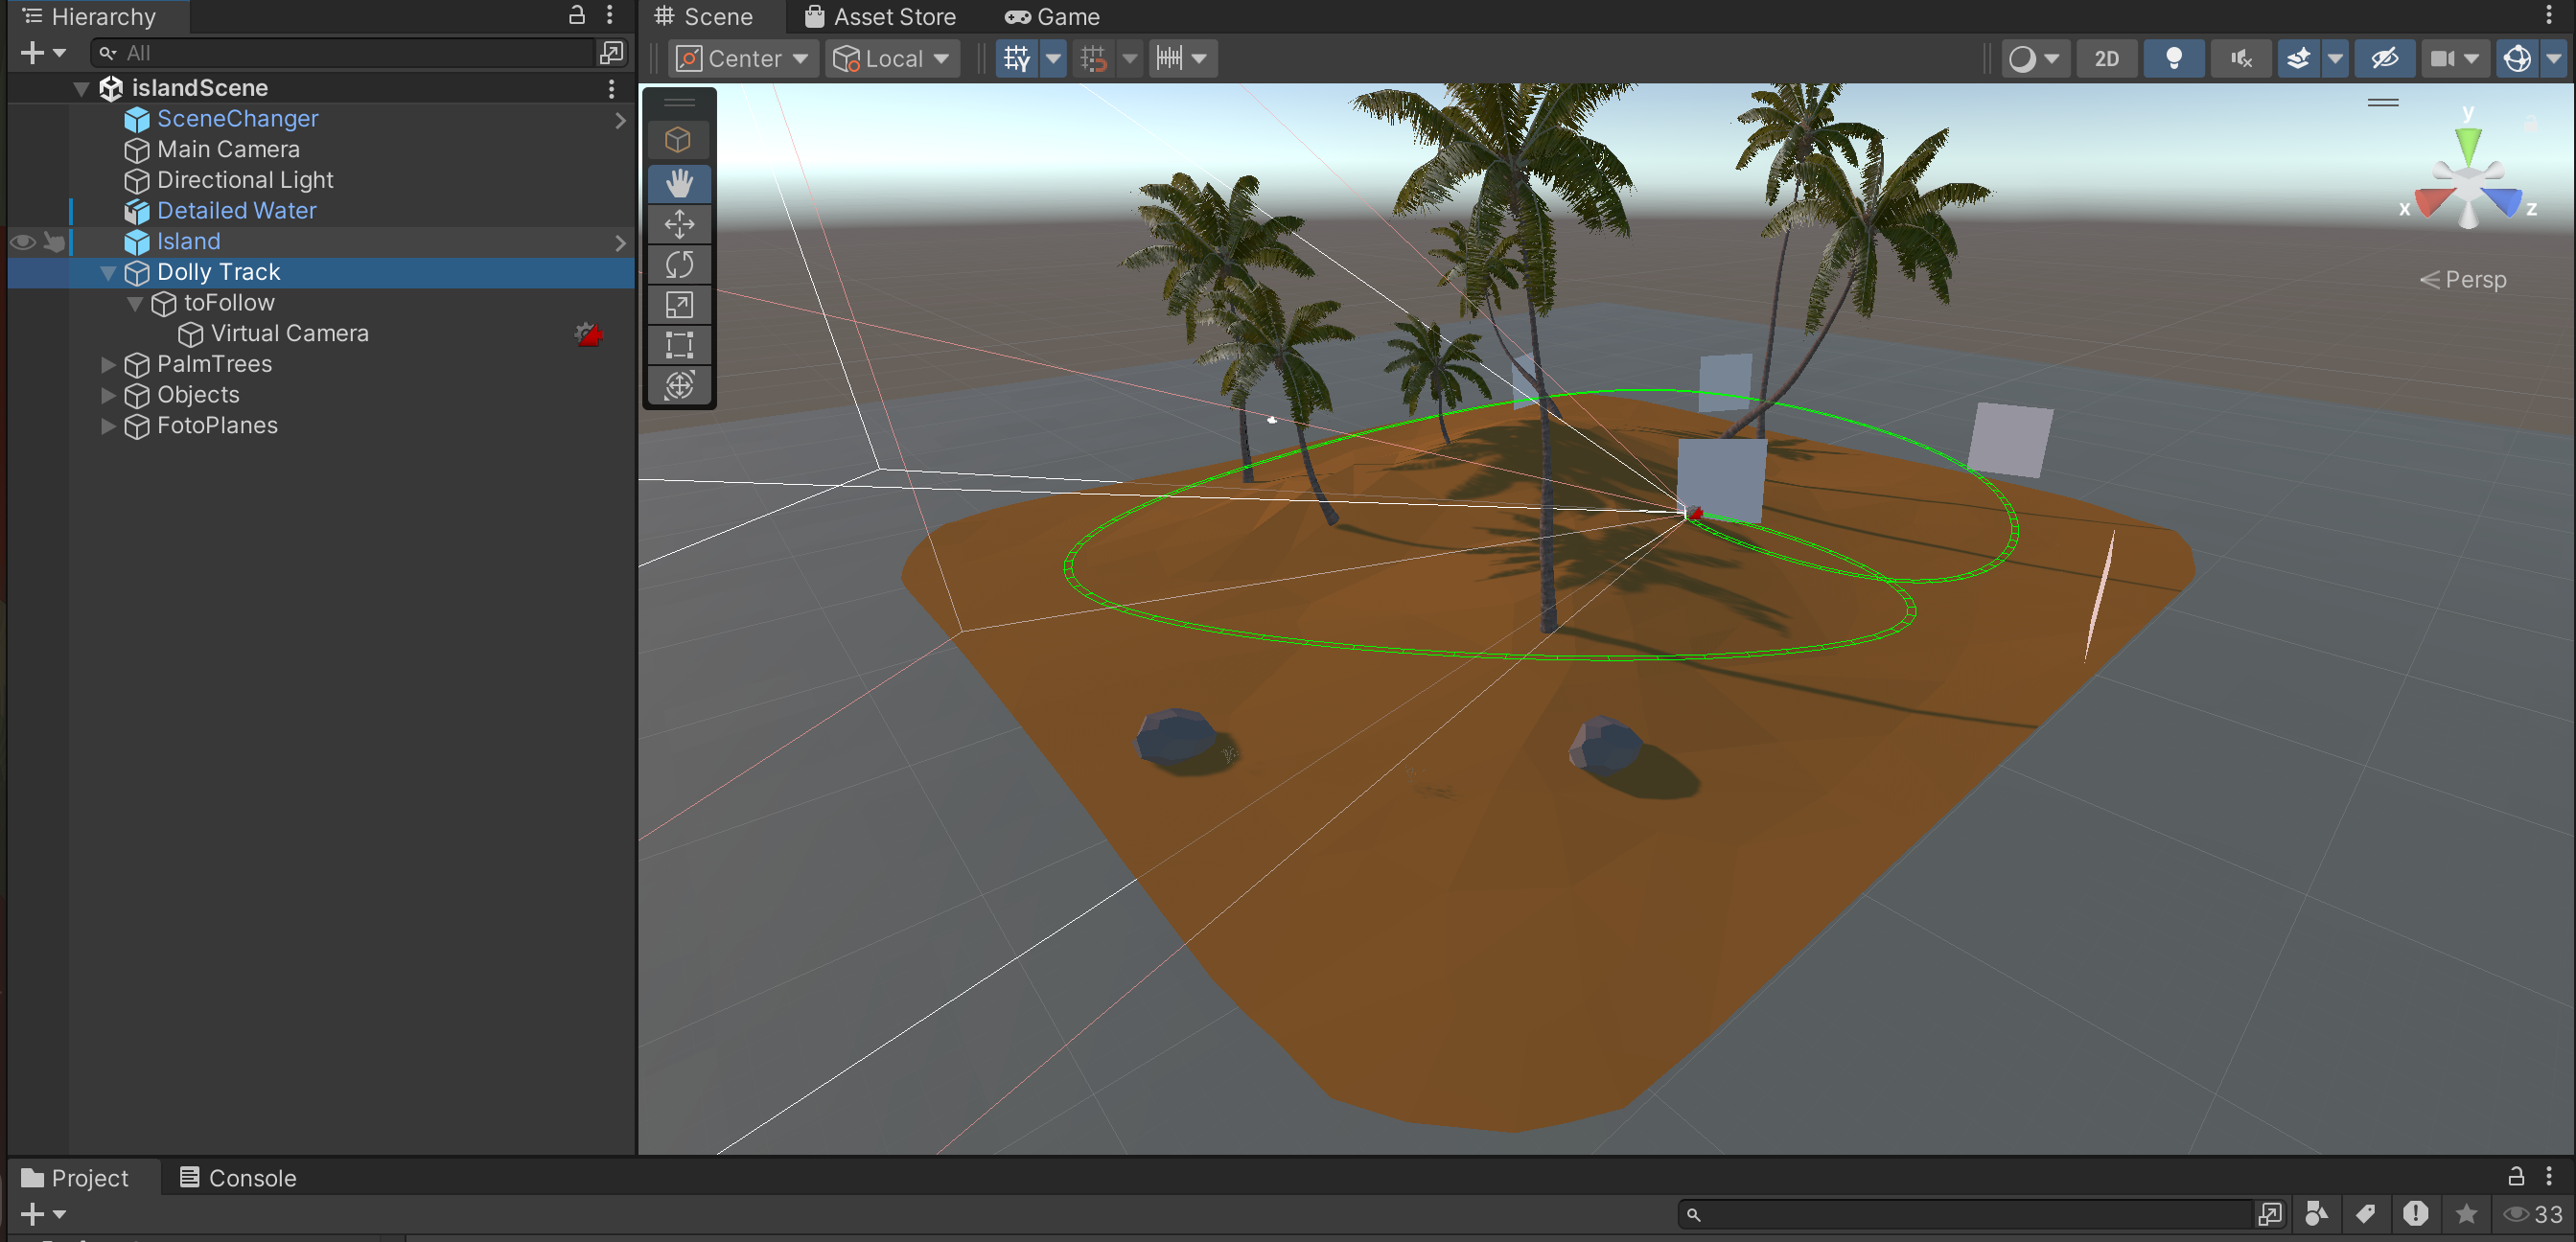
\includegraphics[scale=0.15]{pics/unity-edit-island.png}
    \caption{Entwicklung in Unity: Die Insel Szene}
    \label{fig:unity-edit-island}
\end{figure}


Die Wanderung selbst wird durch die Verwendung des Konzepts des Dolly Track (siehe Abschnitt \ref{subsec:unity-dolly-track}) durchgeführt. Die Nutzer erleben einen Inselspaziergang mit Sonne, Strand und Meer, während sie an den Bildern ihrer Erinnerungen vorüberschreiten.


\subsection{Erweiterbarkeit}
\label{subsec:unity-erweiterbarkeit}

Nach dem vorliegenden Konzept kann nun um beliebige Szenen erweitert werden. Die Szenen müssen mehreren Entwicklungsanforderungen und Grundkonzepten folgen. Die größte Freiheit besteht jedoch darin, dass die Szenen zukünftig auch so programmiert werden können, dass man sich beispielsweise selbständig durch die Szene beweigen könnte.

Erste Voraussetzung ist die Darstellung der Bilder mit Hilfe der bereits .......


..... \emph{OFFEN} WEITER, TODO



\begin{spacing}{1}
\chapter{Zusammenfassung}\label{chapter:Zusammenfassung}
\end{spacing}



Mit dem vorgestellten Projekt Memoryland wurde bewiesen, dass ein immersives Erlebnis mit den Fotos erlebbar werden kann. Es wurden zwei Szenen als erste Beispiele in Unity umgesetzt. Die Waldszene soll die Erinnerung an Spaziergänge oder Wanderungen darstellbar machen. Die Inselszene hingegen, ermöglicht die Erinnerung an sonnige Urlaube an Sonne, Sand, Strand und Meer.

Viele weitere Szenen sind einfach umzusetzen und das Backend sowie das Frontend sind so umgesetzt, dass es einfach möglich ist diese zu integrieren. Es ist nahezu kein Aufwand (das Einfügen eines Datensatzes im Backend in der Memoryland-Type Tabelle) im Backend vonnöten und gar kein Aufwand in der Angular-Umsetzung des Frontend. Die Szenen selbst müssen in Unity entsprechend umgesetzt werden und dabei auf die Vorgaben für neue Szenen Rücksicht genommen werden.\footnote{siehe dazu Abschnitt \ref{subsec:unity-erweiterbarkeit}}

.......




\newpage
\pagenumbering{Roman}
\setcounter{page}{\value{RPages}}

\newacronym{guid}{GUID}{Globally Unique Identifier}
\newacronym{ide}{IDE}{Integrated Development Environment}
\newacronym{jit}{JIT}{Just In Time Compiler}
\newacronym{nfc}{NFC}{Near Field Communication}
\newacronym{rfid}{RFID}{Radio Frequency Identification}

% need : https://tex.stackexchange.com/a/536525

% Usage:
% \gls{label} lowercase in text
% \Gls{label} Uppercase in text
% \newacronym{label}{abbrev}{full}
% \newglossaryentry{label}{settings}



%\setlength{\glsdescwidth}{0.8\linewidth}
\glsnogroupskiptrue
\IfStrEq{\thesislang}{de}
{
	\printglossary[title=Glossar,toctitle=Glossar] %,style=long]
}
{
	\printglossary[title=Glossary,toctitle=Glossary] %,style=long]
}
\spacing{1}{
\IfStrEq{\thesislang}{de}
{
	\bibliographystyle{ieeetrande}
}
{
	\bibliographystyle{IEEEtran}
}
\bibliography{bib}
}
\listoffigures
\listoftables
\lstlistoflistings
\appendix
\addchap{Anhang}
\input{./sections/appendix}
\end{document}

